\documentclass[11pt]{amsart}
\usepackage{amsmath,amssymb,amsthm}
\usepackage{graphicx}
\usepackage{placeins}
\usepackage[hidelinks]{hyperref}
\hypersetup{pdftitle={Two notions of tightness for the flat overhand knot},pdfauthor={Yongseok Jang}}
\usepackage{microtype}
\graphicspath{{./}{figs/}}
\allowdisplaybreaks

\theoremstyle{plain}
\newtheorem{theorem}{Theorem}[section]
\newtheorem{lemma}[theorem]{Lemma}
\newtheorem{proposition}[theorem]{Proposition}
\newtheorem{corollary}[theorem]{Corollary}
\theoremstyle{definition}
\newtheorem{definition}[theorem]{Definition}
\newtheorem{observation}[theorem]{Observation}
\theoremstyle{remark}
\newtheorem{remark}[theorem]{Remark}
\newtheorem{mainthm}{Theorem}
\newtheorem{compres}[theorem]{Computational Result}
\renewcommand{\themainthm}{\Alph{mainthm}}

\newcommand{\core}{\ell_{\mathrm{core}}}
\newcommand{\trunc}{L_{\mathrm{trunc}}}
\newcommand{\M}{M(\mathcal{B})}
\newcommand{\Mhon}{M_{\mathrm{hon}}(\mathcal{B})}
\newcommand{\Mplus}{M_{+}(\mathcal{B})}
\newcommand{\Mhat}{\widehat{M}(\mathcal{B})}
\newcommand{\td}{\theta^\dagger}
\newcommand{\Q}{\mathbb{Q}}
\newcommand{\R}{\mathbb{R}}

\title[Two notions of tightness for the flat overhand knot]{Two notions of tightness for the flat overhand knot:\\ Kauffman's pentagon and an $S_6$-algebraic\\ core-length critical state}
\author{Yongseok Jang}
\address{Independent researcher, Republic of Korea}
\email{yongsk0066@gmail.com}
\date{}
\subjclass[2020]{57K10, 52C25, 90C30, 68V15}
\keywords{folded ribbon knot, flat folding, ribbonlength, figure-eight knot, semialgebraic optimization, exact certificates}

\begin{document}

\begin{abstract}
Tying an overhand knot in a paper strip and pulling it tight famously produces a regular pentagon, which Kauffman conjectured minimizes the length-to-width ratio of the flattened truncated trefoil. We model flat folded overhand knots as a five-dimensional semialgebraic moduli space with classified non-penetration walls: six endpoint slivers and a disjunctive taco pair. Two functionals then compete: Kauffman's truncation length $\trunc$, the material that builds the knot, and the core length $\core$, the material pulling extracts; they select different strict local optima on the three-crease branch. For $\trunc$ we prove what is, to our knowledge, the first optimality result toward Kauffman's conjecture: the pentagon is a strict local minimizer on the three-crease branch, certified by an exact Farkas system in powers of the golden ratio. For $\core$ the pentagon is no local minimum: a certified pulling path crosses it and continues to a reachable strict local minimizer $\td$ whose coordinate field has degree twelve over $\Q$ and whose defining sextic has Galois group $S_6$, so the state admits no expression by radicals; its outline is a notched heptagon, and the exact V-notch is a falsifiable prediction separating the two functionals. The framework extends beyond the trefoil: in a numerically identified cell of the four-crease figure-eight branch we certify an exact blocked strict local minimizer, solvable in the quadratic field $\Q(\sqrt{15})$---core length $4\sqrt{15}/3$, a centrally symmetric hexagonal outline, no notch. A realization theorem, a stratified census with certified exclusions and a localized numerical residue, and machine-checked certificate suites support the analysis.
\end{abstract}

\maketitle

\section{Introduction}\label{sec:intro}

\subsection{The experiment and the folklore}
Take a long strip of paper, tie a simple overhand knot in it, pull the two ends gently, and flatten. The knot settles into a shape that looks, strikingly, like a regular pentagon. The observation is old recreational mathematics; the usual explanation exhibits a one-parameter family of flat folded configurations and notes that the regular pentagon sits at its contact-limited endpoint, and the construction has been formalized algebraically in computational origami by Ida, Ghourabi, and Takahashi \cite{ida2015}. Kauffman \cite{kauffman2004} turned the folklore into a precise question. Modelling the flattened knot as a folded ribbon and measuring the \emph{truncation length}---cut the two tails flush with the outer boundary of the flat knot and unfold---he computed, for the pentagonal trefoil,
\begin{equation}\label{eq:kauffman-ratio}
\frac{L}{W}=\frac{4}{\sqrt{5-2\sqrt5}}=5.5055276819\ldots,
\end{equation}
and conjectured this value to be the minimum for the flattened truncated trefoil. In the two decades since, the conjecture has attracted upper-bound constructions in related models but, to our knowledge, no optimality result of any kind: no criticality, no local minimality.

\subsection{Two ways to pull tight}
The folklore sentence---\emph{pull it tight and you get a pentagon}---hides an ambiguity which turns out to be the heart of the matter. Two quantities have equal claim to the name \emph{tightness}:
the truncation length $\trunc$, the total material needed to \emph{build} the flat knot with tails cut flush, a functional of manufacture; and the core length $\core$, the material trapped between the first and the last crease, which is what pulling on the tails monotonically extracts, a functional of tightening. On the standard symmetric family the two narratives coincide, and both end at the pentagon. On the full configuration space they do not. This paper shows that the two functionals select \emph{different} strict local optima on the branch, and that the folklore statement is precisely true for one of them and precisely false for the other.

\subsection{Main results}
We develop the kinematic theory from the bottom up and push every claim to the strongest verification grade available to us.

Within the stated model---piecewise $C^2$ width-one strips, complete movable creases, zero thickness---the tying combinatorics is forced. A tied flat folded long strip needs at least three creases, and with exactly three the knot type is the trefoil and the entire tying data---which piece pairs cross, in which material order, with which over/under pattern, with which crease-slope signs, under which layer order---is unique up to mirror image, by a self-contained argument citing no knot tables. The configuration space of the resulting branch is a five-dimensional semialgebraic set whose non-penetration boundary we classify completely: six endpoint-sliver walls together with a disjunctive taco pair, the latter revealed to be corner contacts of crease pairs.

The pentagon is a contact-mode junction---informally, a mountain pass---for pulling, and the certified tight state beyond it is algebraically wild. On the symmetric slice, tightening terminates at the regular pentagon---the folklore, proved, and machine-checked in Lean---but in the full five-dimensional space an exact Farkas computation exhibits a legal first-order descent direction, and descent continues along a second symmetric family---feasibly and strictly monotonically all the way, by exact resultant--Sturm certificates. That family reduces to a plane curve $N_5(x,h)=0$ whose unique critical point $\td$ generates a coordinate field of degree twelve over $\Q$, with defining sextic of Galois group $S_6$: \emph{the state reached by the certified pulling path cannot be written in radicals, its $x$-coordinate already having none.} Existence, identification, KKT blocking with strictly positive multipliers, and strict local minimality via an exact reduced Hessian are all certified over $\Q(x^\dagger)$.

Kauffman was right, locally, and no other blocked state is certified. At the pentagon the truncation length has exact gradient $(0,\varphi^3,-\varphi^2,\varphi,0)$ in powers of the golden ratio $\varphi=(1+\sqrt5)/2$, with exact Farkas certificates on an invertible wall system in both taco branches, so the pentagon is a \emph{strict} local minimizer of $\trunc$ on the three-crease branch, with linear growth; since $\trunc(\td)=5.582\ldots>5.506\ldots$, the new state is no counterexample to Kauffman's conjecture. Two further theorems close the picture: for open states of the three-crease branch the sheet-separation layer axioms are equivalent to realizability by embedded zero-thickness strips in slabs $\R^2\times[0,\varepsilon]$ with $\varepsilon\to0$, the zero-clearance case being certified at the pentagon and at $\td$, and a stratified census of all $215$ active-set strata---run through two independent implementations and finished with per-candidate interval certificates---finds exactly one certified blocked state, namely $\td$, with the residual components localized and graded.

The broadest message is the dichotomy: \emph{tightest is not a property of a shape but of a functional.} One wall system, one moduli space, and a single change of objective move a strict local optimum from the golden-ratio world of the pentagon to an $S_6$-algebraic notched heptagon. Precise statements are Theorems A--H in Section~\ref{sec:mainresults}.

The program is not confined to the trefoil. At four creases the same enumeration machinery yields a unique irreducible four-crossing code realizing the figure-eight knot, and on its branch the pulling functional is again blocked at an exactly solvable state---this time in the quadratic field $\Q(\sqrt{15})$, with core length $4\sqrt{15}/3$ and a centrally symmetric hexagonal outline tiled by the core passes without a notch; its truncation length recovers exactly Kauffman's conjectured figure-eight value $32/\sqrt{15}$ \cite{kauffman2004}---the value is his, the exact realization, optimality, and reachability are new. The contrast is instructive: one more crossing, and the certified blocked local minimizer---in its numerically identified cell---drops from degree twelve and unsolvable to degree two. Section~\ref{sec:figure8} develops this second instance end to end.

\subsection{Predictions}
The dichotomy is falsifiable. The certified terminal state of the pulling path differs from the pentagon by a V-notch on one edge, with mouth $0.0845w$, legs $0.0514w$, depth $0.0293w$, and reflex angle $249.52^\circ$ for a strip of width $w$---all four determined by exact elements of the sextic subfield $\Q((x^\dagger)^2)$, namely the three squared lengths and the cosine of the angle. On a $2\,$cm tape this is a notch about $1.7\,$mm wide and $0.6\,$mm deep. Moreover, along one certified opening direction our constant-height hairpin construction realizes nearby open states at cost $\Delta\ell\lesssim3.5\,\varepsilon$, the coefficient combining the exact multiplier sum $\sum_j\lambda_{w_j}=4.11\ldots$ with the slab-budget rate; the KKT multipliers are the unit prices of the ramp clearances. This is a construction-specific $O(\varepsilon)$ upper bound; no universal lower bound, and no fixed-thickness exclusion of $\td$, is proved. Real paper may instead lock at the pentagon, through friction at eight simultaneous contacts and pinned creases; that would itself be this model's explanation of the folklore, and the notch remains the discriminating signal rather than a guaranteed outcome. See Section~\ref{sec:shape}.

\subsection{Methods and verification}
Every structural claim in this project was probed numerically before being asserted, then promoted along a fixed ladder: multistart numerics; high-precision identification by PSLQ \cite{fba1999} over the relevant number field; exact verification in quotient fields $\Q[x]/(p)$; interval arithmetic (interval Newton, Krawczyk) for signs and existence; and, for the algebraic core, machine-checked proofs in Lean~4/Mathlib \cite{mathlib2020}---a discipline that at one point overturned one of our own intermediate claims and thereby uncovered $\td$ (Remark~\ref{rem:methods}). Internal verification is not journal peer review; the complete suite, with pinned dependency versions and reproduction instructions, accompanies the paper as ancillary material \cite{anc}, and Appendix~\ref{app:suite} describes it.

\subsection{Related work}
Kauffman's paper \cite{kauffman2004} is the origin of the truncated functional; among the works surveyed here we have found no prior optimality or non-optimality result for the pentagon. Ida, Ghourabi, and Takahashi \cite{ida2015} formalized the classical three-fold construction, proving algebraically---with Gr\"obner-basis certificates---that the resulting polygon is regular when the terminal contact points coincide, and treating pentagonal and heptagonal knot folds; their work concerns the construction and verification of a prescribed fold, and does not formulate the deformation space, a tightening functional, or the contact-constrained optimality problem studied here. The modern folded-ribbon literature studies \emph{closed} folded ribbonlength through upper-bound constructions across all diagrams---Denne and coauthors \cite{denne2020}, with the survey \cite{denne2018}; recently Chen, Denne, Patterson, and Patterson \cite{chen2025}; general linear upper bounds in the crossing number by Kim, No, and Yoo \cite{kimnoyoo2026}, subsequently sharpened through Yoo's four-page index \cite{yoo2026b}; bounded ribbonlength for knot families and multi-twist M\"obius bands by Denne and Patterson \cite{dennepatterson2025}; and, for alternating links with bipartite dual graphs, Yoo \cite{yoo2026}---a different quantity and a different problem from our fixed-branch, open and truncated kinematics. The immersed thread \cite{immersed2020,ayala2025} proves exact minima for $C^1$ immersed disk diagrams via vertex tension balance, the immersed cousin of our wall-KKT balance, with no folds and hence no overhand branch. Layer conditions for flat folding go back to Justin \cite{justin1997}, Hull \cite{hull2002}, and Demaine--O'Rourke \cite{demaine2007}; monotone-path formalizations to Connelly, Demaine, and Rote \cite{cdr2003}; contact-force criticality for ropelength to Schuricht and von der Mosel \cite{svdm2004} and Cantarella, Kusner, and Sullivan \cite{cks2002}. The combination pursued here---a fixed tying branch, a moduli space with classified contact walls, two tightness functionals, and end-to-end certificates---appears to be new.

\subsection{Organization}
Section~\ref{sec:mainresults} states the main theorems. Sections~\ref{sec:model}--\ref{sec:census} develop the model, the walls, the tightening theory, the second family, the dichotomy, realization, the shape, and the census. Section~\ref{sec:figure8} carries the program to the figure-eight knot. Section~\ref{sec:open} collects open problems. Appendix~\ref{app:suite} documents the verification suite and Appendix~\ref{app:lean} the Lean formalization.

\section{Main theorems}\label{sec:mainresults}

Throughout, the material is a width-one long strip folded flat at three complete creases along the overhand (long trefoil) branch $\mathcal B$. States are pairs $(f_\theta,\lambda)$ of a planar placement and a layer order, with passes labelled $A,B,C,D$ in material order and coordinates $\theta=(x,g,h,a,b)\in\M\subset\R^5$. On the computational chamber $\M=\Mhat$ the working constraints are the six sliver walls $w_1,w_4,w_5,w_6,w_7,w_8$ and the unwindowed taco pair $w_9,w_{10}$, feasibility being $\{w_9\ge0\}\cup\{w_{10}\ge0\}$; on the honest moduli the taco faces are windowed, as stated in Theorem~\ref{mainthm:moduli}; the layer order $B>D>A>C$ is forced by the branch data. Creases are movable fold lines: a tightening path varies crease positions and angles continuously while preserving the branch data; there are no material-pinned creases and no refolding. A valid state is \emph{blocked} when $\nabla\core$ lies in the cone generated by the gradients of its active walls, taken within the relevant taco branch. Precise definitions occupy Section~\ref{sec:model}.

\begin{mainthm}[fold number and rigidity of the tying]\label{mainthm:fold}
A tied flat folded long strip, in the general-position class of Definition~\textup{\ref{def:gp}}, has at least three creases. With exactly three, the knot type is the left- or right-handed trefoil, and the full tying data---crossing pairs, material passage word $\mathtt{XYZXYZ}$, alternating over/under pattern, alternating crease-slope signs $\epsilon=(+,-,+)$, layer order $B>D>A>C$---is unique up to mirror image. The proof cites no knot classification tables.
\end{mainthm}

\begin{mainthm}[moduli and walls]\label{mainthm:moduli}
The honest moduli $\Mhon$, its positive-taco locus $\Mplus$, and the computational chamber $\M=\Mhat$ are five-dimensional semialgebraic sets with $\Mplus\subseteq\Mhat\subseteq\Mhon$. The non-penetration boundary of $\Mhon$ consists of the six sliver walls and the two taco faces windowed by $0\le u\le1$ and $0\le t\le1$; the chamber is cut out by their unwindowed extensions, capture faces that bound no contact; all eight wall functions admit polynomial representatives with integer coefficients, and $\core$ is a rational function of $\theta$. The taco walls are corner contacts of crease pairs: $w_9=w_{10}=0$ exactly when $Q_0=F$, a three-dimensional manifold $\mathcal F$ whose intersection with $\{w_1=w_4=0\}$ is the standard slice, on which all six of $w_1,w_4,w_7,w_8,w_9,w_{10}$ vanish identically.
\end{mainthm}

\begin{mainthm}[the pentagonal contact-mode junction]\label{mainthm:pass}
On the symmetric slice, tightening terminates at the regular pentagon. At the pentagon, $\nabla\core=\tfrac12\mathbf 1$ exactly, and $\nabla\core$ lies in no subcone of the active wall gradients in either taco branch: an explicit first-order descent direction exists along a second symmetric family, and the pentagon is the crossing corner of two symmetric one-parameter families. Along the second family, parametrized by the branch through $\td$ of the plane curve $N_5(x,h)=0$ of Theorem~\textup{\ref{mainthm:dagger}}, the four remaining walls satisfy $w_7=w_8>0$ and $w_9=w_{10}>0$ strictly between the endpoints, vanishing exactly at the pentagon, and $\core$ is strictly monotone with derivative vanishing exactly at $\td$: exact endpoint identities, five root-free resultant--Sturm certificates on an interval containing $[x^\dagger,x_0]$, and an interval-certified interior sample. Hence descent from the pentagon along the second family reaches $\td$ through valid states of the branch---branch preservation being certified by a further family of root-free resultants---with strictly decreasing core length, and the reverse of the opening segment at the pentagon supplies the slack start: $\td$ is reachable from slack states, and \emph{tight} in the sense of Definition~\textup{\ref{def:pull}}.
\end{mainthm}

\begin{mainthm}[the tight state]\label{mainthm:dagger}
The second family reduces to the plane curve $N_5(x,h)=0$ with $a=h$, $b=(x^2+1)/(2x)$ and $\core=h+b$; write $\ell(x)$ for the resulting restriction of $\core$ to the family. Its unique critical point $\td$ satisfies: $x^\dagger$ has minimal polynomial $p_x=x^{12}+4x^{10}-7x^4+20x^2-2$; the field $\Q(\td)=\Q(x^\dagger)$ has degree twelve; the Galois group of the even subfield generator is $S_6$, so $\td$ admits no radical expression; and $\sqrt5\notin\Q(x^\dagger)$. The KKT multipliers at $\td$ are explicit elements of $\Q(x^\dagger)$, strictly positive, with $\lambda_{w_1}=\lambda_{w_4}$ identically and $\lambda_{w_5}$ in the sextic subfield; and $\td$ is a strict local minimizer of $\core$, the reduced Hessian on the one-dimensional critical cone being the exact element
\begin{multline*}
\ell''(x^\dagger)=\Bigl(\tfrac{2483}{24}x^{11}+\tfrac{849}{2}x^{9}+\tfrac{175}{4}x^{7}+\tfrac{53}{12}x^{5}-\tfrac{17377}{24}x^{3}\\
+\tfrac{7977}{4}x\Bigr)\Big|_{x=x^\dagger}=618.248\ldots>0.
\end{multline*}
\end{mainthm}

\begin{mainthm}[first optimality toward Kauffman's conjecture]\label{mainthm:kauffman}
At the pentagon, $\nabla\trunc=(0,\varphi^3,-\varphi^2,\varphi,0)$ exactly, and both taco branches admit exact Farkas certificates with five strictly positive multipliers on an invertible five-by-five wall system. Hence every nonzero feasible direction strictly increases $\trunc$, and the pentagon is a strict local minimizer of the truncation length on the three-crease branch, with linear growth. In contrast, $\trunc(\td)=5.5818\ldots>4/\sqrt{5-2\sqrt5}$: the two functionals select different strict local optima.
\end{mainthm}

\begin{mainthm}[realization completeness for the three-crease branch]\label{mainthm:realization}
For $\mathcal B$-states, in the sheet-separation layer model: necessity is unconditional---every limit realization by embeddings into $\R^2\times[0,\varepsilon_k]$ with $\varepsilon_k\downarrow0$ satisfies the combinatorial axioms; open states satisfy the converse unconditionally, admitting strong $\varepsilon$-realizations for all $\varepsilon<\varepsilon_0(\theta)=\frac{2}{\pi\Lambda}\min(m_{\mathrm{mat}},2c_{\mathrm{nb}},c_{\mathrm{cr}})$; for zero-clearance states the converse holds under the opening hypothesis of the text, which is exactly certified at the pentagonal and dagger states, so that both are limits of open realized states, with exact rank and positivity certificates.
\end{mainthm}

\begin{mainthm}[stratified census]\label{mainthm:census}
\textup{(1) [proved]} Every tight state satisfying the Mangasarian--Fromovitz constraint qualification is blocked, and every blocked point appears as a KKT root of one of $215$ active-set strata---all active sets of at most five walls, both-taco sets included as redundant super-captures, less the four subsets of $\{w_4,w_6\}$ excluded by $x$-independence---and by Carath\'eodory at most one taco wall is ever needed for capture. \textup{(2) [exact and interval certificates]} Within these strata, the pentagon appears as a root in $20$ of them and is excluded wholesale by the single exact Farkas certificate of Theorem~\textup{\ref{mainthm:pass}}; all $72$ candidates admitting certifiable regular roots are excluded by interval certificates; $\td$ is the unique \emph{certified} blocked state. 
\end{mainthm}

\begin{compres}[Computational census evidence]\label{compres:censusintro}
That no blocked state escapes the remaining numerical components---per-stratum root coverage of the double-implementation harvest, absence of valid non-MFCQ points, on-branch scale calibration, and the $32$ Krawczyk-inconclusive candidates, each of which violates a true wall numerically---is computational evidence, localized in Section~\ref{sec:census}. Reachability of $\td$ by a general descent from an arbitrary slack state, as opposed to along the certified path of Theorem~\textup{\ref{mainthm:pass}}, is a separate, numerically supported statement.
\end{compres}

\begin{mainthm}[an exact blocked hexagon on the figure-eight branch]\label{mainthm:hex}
At four creases the enumeration of Theorem~\textup{\ref{mainthm:fold}} yields a unique irreducible four-crossing code, and exactly two of its sixteen over/under assignments---a mirror pair---realize the figure-eight knot $4_1$. In the numerically identified cell of the resulting seven-dimensional branch described below---an $8\times10^6$-sample sweep finds valid width-one flat folded states, all in a single cell, self-mirror under material reversal, with layer order $P_1>P_4>P_2>P_0>P_3$ up to the top-bottom flip---the following centrally symmetric state $\theta^*_{4_1}$, exactly solvable in $\Q(\sqrt{15})$, is a valid, reachable, strict local minimizer of $\core$:
\begin{gather*}
\cos\tau_1=-\tfrac14,\qquad \tau_2=2\pi-2\tau_1=-\tau_3,\qquad \tau_4=-\tau_1,\\
(L_1,L_2,L_3)=\tfrac{1}{\sqrt{15}}\,(6,8,6),\qquad \core=\tfrac{4\sqrt{15}}{3}.
\end{gather*}
Its eight active contacts vanish exactly, its KKT multipliers on an invertible seven-generator subsystem of the eight active gradients are positive elements of $\Q(\sqrt{15})$, and first-order sufficiency upgrades blocking to \emph{strict} local minimality of $\core$. Its core outline is a centrally symmetric hexagon with sides $\tfrac{2\sqrt{10}}5$ and $\tfrac{4}{\sqrt{15}}$ and interior angles $\arccos(-\tfrac14)$ and $\pi-\tfrac12\arccos(-\tfrac14)$, which the three core passes tile without a notch, exactly; and the truncation length is $\trunc(\theta^*_{4_1})=\tfrac{32\sqrt{15}}{15}$, each truncation stub equal to $L_1$, so that $\trunc/\core=\tfrac85$ exactly; the value $32/\sqrt{15}$ is precisely the figure-eight ribbon length conjectured by Kauffman \cite{kauffman2004}. The state itself is certified valid: all thirty-nine candidate contact margins of the branch inventory, evaluated at $\theta^*_{4_1}$ in $\Q(\sqrt{15})$, come out exactly zero for the eight active contacts and strictly positive for the other thirty-one, so the existence of valid states is exact, witnessed by $\theta^*_{4_1}$. Moreover the exact opening direction furnishes a slack start whose reversal reaches $\theta^*_{4_1}$, which is therefore reachable and \emph{tight} in the sense of Definition~\textup{\ref{def:pull}}. Exhaustiveness of the cell within the sweep and convergence of \emph{generic} descent are numerical.
\end{mainthm}

\section{The model}\label{sec:model}

\subsection{Material, placement, and regularity}

Paper is modelled as an inextensible surface of zero thickness. For $0<w<L$ the \emph{strip} is the rectangle $R_{L,w}=[0,L]\times[-\tfrac w2,\tfrac w2]$ carrying the Euclidean metric; all the information the material holds at this stage is intrinsic, namely lengths and angles measured along the sheet. The sheet has zero material thickness throughout. Non-penetration means injectivity of the realized surface, and $\varepsilon$ bounds the height of its containing slab; it is neither material thickness nor a minimum separation between sheets. A positive-thickness material model would require additional assumptions.

\begin{definition}[Admissible configuration]\label{def:admissible}
A map $F\colon R_{L,w}\to\R^3$ is \emph{inextensible} where it is differentiable if $(DF)^{T}DF=I_2$, equivalently if it preserves the length of every material curve. It is an \emph{admissible configuration} if there is a finite graph $\Gamma\subset R_{L,w}$, the \emph{crease pattern}, such that $F$ is a $C^2$ inextensible immersion on every connected component of $R_{L,w}\setminus\Gamma$, called a \emph{panel}, and $F$ is continuous on all of $R_{L,w}$.
\end{definition}

\begin{remark}[The regularity class is a modelling decision]\label{rem:regularity}
Inextensibility alone forces nothing. By the Nash--Kuiper theorem \cite{nash1954,kuiper1955} a $C^1$ isometric embedding of a strip exists inside a ball of arbitrarily small radius, so paper-likeness is not a consequence of not stretching. It is the class of Definition~\ref{def:admissible}, piecewise $C^2$ with finitely many creases, that makes the Gauss curvature argument available on panels, so that a panel is developable, hence ruled \cite{docarmo1976}, and flat states are rigid. Every theorem below is a theorem about this class.
\end{remark}

On a \emph{flat} configuration the class collapses to something completely rigid: each panel is a rigid piece of the plane, each crease is a straight line, and adjacent panels are related by reflection in that line. This is a structure theorem, not a definition, and it has one consequence that organizes the whole paper: the continuous information carried by a flat folded state is exactly the positions of the creases, and everything else is combinatorial. That is why a finite-dimensional coordinate chart exists at all (Proposition~\ref{prop:dim}).

\subsection{Long strips, flat folded states, and diagrams}

To speak of knotting we replace the finite strip by the long strip $R_w=\R\times[-\tfrac w2,\tfrac w2]$. A \emph{long-strip placement} is an admissible configuration $F\colon R_w\to\R^3$ with finite bounded crease pattern whose image agrees, outside some ball, with two straight half-infinite flat ribbons. Admissibility asks immersion, not injectivity, so a placement's centreline may self-intersect; a placement whose centreline is injective---then automatically a proper embedding, being straight outside a ball---is a \emph{spatial long-strip knot configuration}, a \emph{long-strip configuration} for short. The \emph{knot type} of a spatial long-strip knot configuration is the ambient-isotopy class of its centreline, a classical long knot; planar folded states, whose centrelines self-intersect by design, are assigned no spatial knot type directly, their tiedness being the diagrammatic one used throughout; the ribbon carries strictly more data---framing, annulus versus M\"obius after closure---which Remark~\ref{rem:framing} records and which this paper does not use. The two straight ends are the topological substitute for holding the strip in one's hands: a knot cannot escape off the end. The price is that the existence threshold, that is how long a strip must be before a given knot can be tied in it, is excluded from the model; that question belongs to ribbonlength theory \cite{kauffman2004,denne2020,chen2025} and is not treated here.

\begin{proposition}[Long knots and their closures]\label{prop:closure}
The centreline of a spatial long-strip knot configuration is, by definition, a proper embedding $\gamma\colon\R\hookrightarrow\R^3$ that is straight outside a ball; adding the point at infinity extends it canonically to an embedding $\bar\gamma\colon S^1\hookrightarrow S^3=\R^3\cup\{\infty\}$, tame at $\infty$ because the two tails are straight. Centreline knot types of long-strip configurations correspond bijectively, via $\gamma\mapsto\bar\gamma$, to classical closed knot types.
\end{proposition}

\begin{proof}
Compactness at infinity makes the closure canonical: the one-point compactification requires no choice of closing arc, and an ambient isotopy of $\R^3$ through long-strip configurations, being straight outside a ball, extends to an ambient isotopy of $S^3$ fixing $\infty$. Conversely every classical knot type contains a representative straight outside a ball, which reads back as a long-strip centreline.
\end{proof}

\begin{remark}[Framing ledger]\label{rem:framing}
A ribbon carries more than its centreline: whether the closed-up ribbon is an annulus or a M\"obius band is determined by the parity of the crease number together with the writhe of the diagram. This is bookkeeping parallel to, and not part of, the knot type, and it is not used below.
\end{remark}

\begin{definition}[Flat folded state]\label{def:flatstate}
A \emph{flat folded state} is a pair $(f,\lambda)$ in which $f\colon R_w\to\R^2$ is a planar long-strip placement all of whose creases are \emph{complete}, meaning that in material coordinates each crease is a chord joining the two long edges and hence crosses the centreline, and $\lambda$ is a \emph{layer order}: a local linear order on the material points sharing a plane point, subject to the standard non-crossing axioms of flat origami \cite{justin1997,hull2002,demaine2007}. The instance of those axioms used in this paper is Definition~\ref{def:axiom}.
\end{definition}

\begin{definition}[Tying data]\label{def:tying}
Erasing the continuous information from a flat folded state leaves the combinatorial type $(n,\epsilon_1\cdots\epsilon_n,\lambda)$, where $n$ is the number of creases in material order, $\epsilon_i\in\{+,-\}$ is the \emph{tilt sign}, also called the crease-slope sign, of crease $i$, and $\lambda$ is the combinatorial layer order. The space of flat folded states realizing a given tying datum is its (honest) moduli space; for the overhand branch, Section~\ref{sec:moduli} names it $\Mhon$ and fixes the working subspaces $\Mplus\subseteq\Mhat$ used throughout.
\end{definition}

The basic split of the theory is contained in that definition: the tying is a discrete datum, a shape is a point of the honest moduli $\Mhon$, and tightening is a motion inside it; the optimization of this paper is carried out on the working chamber $\M=\Mhat$, with the local theorems taking place in $\Mplus$ (Section~\ref{sec:moduli}); Figure~\ref{fig:notation} displays the two sides of the split.

\begin{figure}[t]
\centering
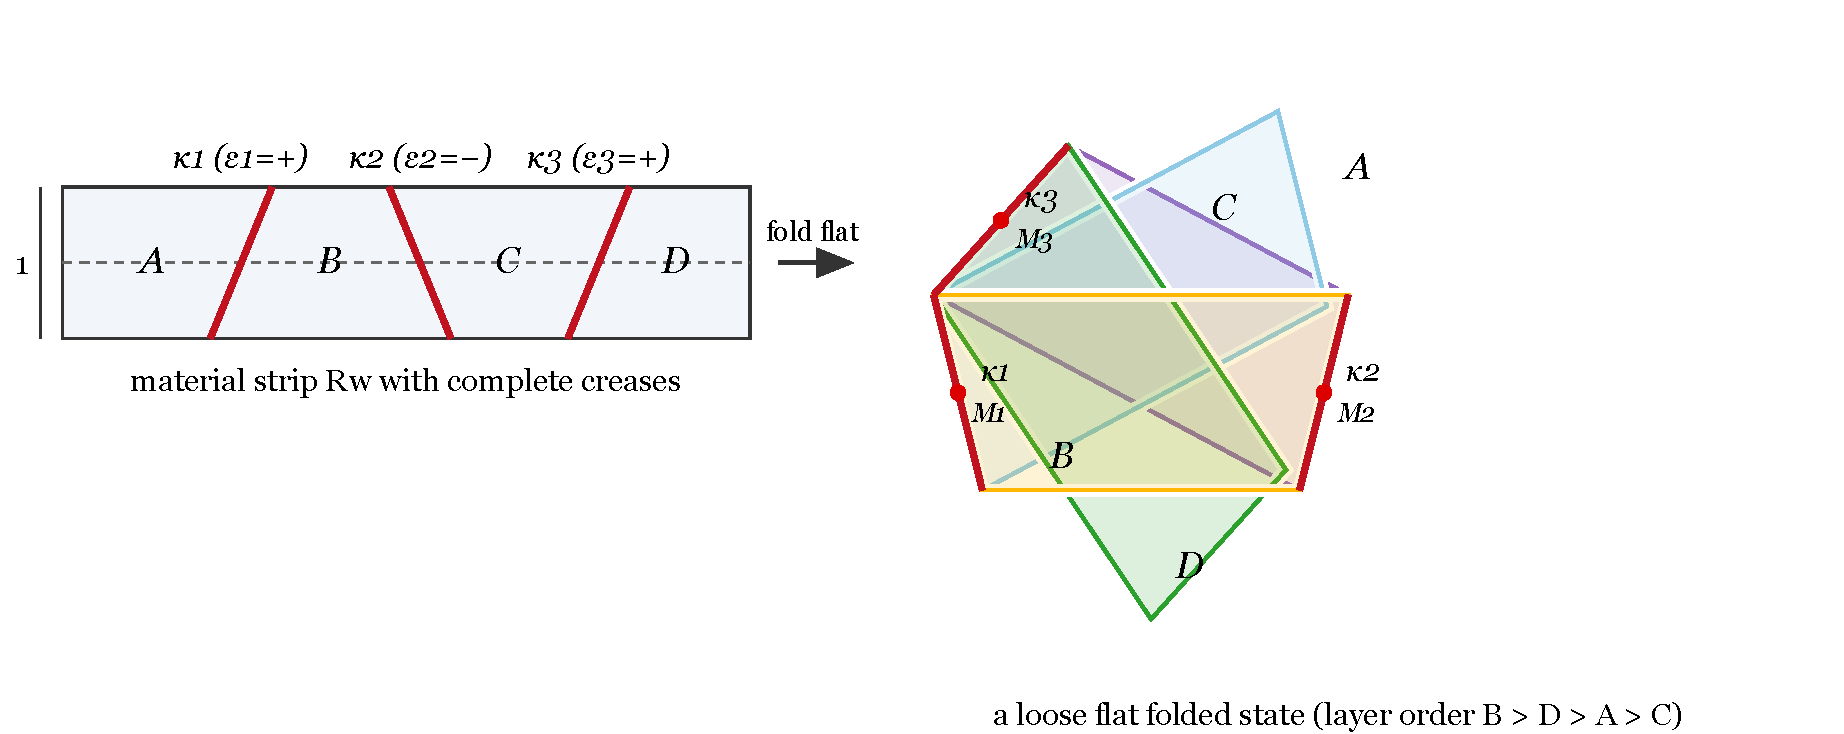
\includegraphics[width=0.98\linewidth]{figs/fig0-notation.pdf}
\caption{The split into tying and shape. Left: material coordinates---the long strip $R_w$, three complete crease chords $\kappa_1,\kappa_2,\kappa_3$ with tilt signs $\epsilon$, and the passes $A,B,C,D$ they bound. Right: a loose flat folded state of the overhand branch realizing this datum, drawn from exact slice coordinates: panels are rigid, creases (heavy) are straight chords with fold points $M_i$ on the centreline, and the layer order $B>D>A>C$ decides every crossing.}
\label{fig:notation}
\end{figure}

\begin{observation}\label{obs:diagram}
A flat folded state \emph{is} a knot diagram. The image of the centreline is a planar polyline, straight on each panel by rigidity; in general position its self-intersections are finitely many transverse double points, and at each of them the layer order $\lambda$ of the two panels involved decides which strand is over. Thus $(f,\lambda)$ determines a long-knot diagram $D(f,\lambda)$ with no auxiliary projection and no further interpretation.
\end{observation}

We call $(f,\lambda)$ \emph{tied} if $D(f,\lambda)$ represents a nontrivial knot type.

\begin{remark}[Crease mobility]\label{rem:mobility}
A tightening path varies the positions \emph{and} the angles of the creases continuously, preserving only the crease number and the combinatorial datum. The creases of this model are therefore movable fold lines, idealized lines of concentrated curvature that roll along the material, and not plastic scars pinned to material coordinates. The pinned-crease model and the refolding model, in which an existing crease is undone and a new one made, are different problems, and any comparison with a physical experiment must say which model is meant.
\end{remark}

\subsection{The fold number and the rigidity of the tying}

Throughout this subsection $(f,\lambda)$ is a flat folded state with $n$ complete creases, whose centreline pieces are $P_0,\dots,P_n$, with $P_0$ and $P_n$ rays and the rest segments.

\begin{definition}[General position]\label{def:gp}
The state is in \emph{general position} (GP) if no two pieces overlap in more than one point, and all double points of the centreline are transverse, pairwise distinct, and at positive distance from fold points and crease segments.
\end{definition}

General position is not an extra hypothesis imposed for convenience. It is precisely the condition under which the diagram of Observation~\ref{obs:diagram} is well defined, and being tied presupposes that diagram; a degenerate fold angle, for instance, produces a collinear overlap of adjacent pieces and is excluded by the first clause. In this sense a tied state means, by definition, a state in general position.

\begin{remark}[Numerical remark]\label{rem:gpaudit}
The general-position margins are comfortable at every state we have examined. At the regular pentagon the minimum crossing angle is $72.0^\circ$ and the smallest crossing-to-crease distance is $0.500$ in units of the strip width; at the tight state $\td$ the corresponding values are $69.5^\circ$ and $0.517$, and at a loose slice state $56.1^\circ$ and $0.658$. Over $2000$ random valid states the minimum crossing angle is $28.4^\circ$ and the crossing-to-crease distance never drops below $0.506$; in every state audited the crossing pairs are exactly $\{(P_0,P_2),(P_0,P_3),(P_1,P_3)\}$, with no adjacent-pair crossing and no collinear pair. These are numerical audits, recorded in the ancillary verification suite \cite{anc}.
\end{remark}

\begin{lemma}[Straightness and the crossing bound]\label{lem:crossbound}
Under GP the crossings of $D(f,\lambda)$ are exactly the transverse double points of non-adjacent pairs of pieces, and each such pair crosses at most once. Hence the number of crossings is at most $\binom{n+1}2-n=\tfrac{n(n-1)}2$.
\end{lemma}

\begin{proof}
Each panel is rigid, so $P_i\subset\Lambda_i$ for a line $\Lambda_i$ and no piece meets itself. Two distinct lines meet at most once, and GP makes the meeting transverse. For an adjacent pair, $\Lambda_{i+1}=\rho_i(\Lambda_i)$ with $\rho_i$ the reflection in the crease line $\ell_i$, and the fold point $M_i\in\Lambda_i\cap\ell_i$ is fixed by $\rho_i$, so $M_i\in\Lambda_i\cap\Lambda_{i+1}$. If $\Lambda_{i+1}\ne\Lambda_i$ this is their only intersection, and it is a fold vertex shared as an endpoint rather than a double point. The remaining case $\Lambda_{i+1}=\Lambda_i$ means $\rho_i(\Lambda_i)=\Lambda_i$, hence either $\Lambda_i=\ell_i$, which is impossible because a complete crease is a chord joining the two long edges and is therefore transverse to the centreline, or $\Lambda_i\perp\ell_i$, a perpendicular fold-back in which two adjacent pieces overlap collinearly and which GP excludes.
\end{proof}

In particular $n\le2$ permits at most one crossing, and $n=3$ at most three.

\begin{lemma}[Crossing-preserving closure]\label{lem:closureop}
Let $\Delta$ be a disc containing all creases and all crossings in its interior. Then $D\setminus\Delta$ consists of two straight tails, each meeting $\partial\Delta$ once and transversally; joining the two cut points by an arc of $\partial\Delta$ produces a closed generic curve $\widehat D$ with no new crossings, whose knot type is the closure of the long knot represented by $D$ and whose Gauss code, read cyclically, is unchanged.
\end{lemma}

\begin{proof}
Choose the radius large enough that all fold points and crossings lie in the interior. The disc is convex, so the intermediate segments, whose endpoints are interior fold points, lie wholly inside it, while each of the two rays leaves from an interior point, crosses $\partial\Delta$ exactly once transversally, and stays outside afterwards. Hence the only intersections of the tails with $\partial\Delta$ are the two cut points, and the interior of the joining arc misses $D$ entirely. Independence of the closure is Proposition~\ref{prop:closure}.
\end{proof}

\begin{lemma}[Gauss parity]\label{lem:parity}
In the Gauss code of a closed generic plane curve, the number of symbols strictly between the two occurrences of any given symbol is even.
\end{lemma}

\begin{proof}
A crossing $c$ splits the curve into two closed loops $\gamma_1,\gamma_2$. In a cyclic code it does not matter which of the two arcs is counted, since the two counts differ by an even number. The symbols between the two occurrences of $c$ are the crossing events on $\gamma_1$; a self-crossing of $\gamma_1$ contributes two such events and a crossing with $\gamma_2$ contributes one, so the parity in question equals $|\gamma_1\cap\gamma_2|\bmod2$. Rounding the corner at $c$ separates $\gamma_1$ and $\gamma_2$ near $c$ into two transverse closed curves, and two closed curves in the plane meet in an even number of points, the $\mathbb Z/2$ intersection number vanishing by the Jordan curve theorem.
\end{proof}

\begin{lemma}[At most two crossings implies unknotted]\label{lem:twocrossings}
A long or closed diagram with at most two crossings represents the trivial knot; hence a nontrivial knot satisfies $c(K)\ge3$.
\end{lemma}

\begin{proof}
Close the diagram up by Lemma~\ref{lem:closureop}. With one crossing the code is $XX$. With two crossings the cyclic code is, up to renaming, of type $XXYY$, which contains an adjacent repeat, or $XYXY$; the latter has exactly one symbol, an odd number, between the two occurrences of $X$, and is excluded by Lemma~\ref{lem:parity}. Every remaining code has an adjacent repeat, so some crossing is traversed twice consecutively and the loop between the two passages carries no crossing event. That loop is an embedded Jordan curve, and the rest of the curve is a connected set meeting it only at the vertex, so one of the two complementary discs is free of the diagram; a first Reidemeister move across that disc on $S^2$ removes one crossing. Induction terminates at zero crossings. The underlying enumeration of codes is also machine-checked in the ancillary verification suite \cite{anc}.
\end{proof}

\begin{lemma}[Passage order for three creases]\label{lem:passage}
Let $n=3$ and suppose the three non-adjacent pairs $X=(P_0,P_2)$, $Y=(P_0,P_3)$ and $Z=(P_1,P_3)$ each cross exactly once. In material coordinates the passages follow the block order $P_0<P_1<P_2<P_3$, so the only freedom is the order of the two passages inside $P_0$ and of the two inside $P_3$, giving four codes. Exactly one of them is realizable in the plane, namely $\mathtt{XYZXYZ}$.
\end{lemma}

\begin{proof}
Apply Lemma~\ref{lem:parity} to the closed code. In $\mathtt{YXZXYZ}$ there are three symbols, $X,Z,X$, between the two occurrences of $Y$; in $\mathtt{XYZXZY}$ likewise three between the two occurrences of $Y$; and $\mathtt{YXZXZY}$ has one between the two occurrences of $X$. Only $\mathtt{XYZXYZ}$ has an even count, namely two, for every symbol.
\end{proof}

\begin{lemma}[Shadow rigidity]\label{lem:shadow}
The shadow of any closed realization of $\mathtt{XYZXYZ}$, that is the four-valent plane graph obtained by forgetting over and under, is unique on $S^2$ up to homeomorphism and mirror, and equals the shadow of the closure of the two-strand braid $\sigma_1^3$.
\end{lemma}

\begin{proof}
There are three vertices of valence four and six edges, hence five faces on $S^2$. The code has no adjacent repeat, so there are no loop edges and no monogons: every face has degree at least two and the degrees sum to $12$. Absence of loops gives, at each vertex, $m_{XY}+m_{XZ}=m_{XY}+m_{YZ}=m_{YZ}+m_{XZ}=4$, whence $m_{XY}=m_{YZ}=m_{ZX}=2$, a doubled triangle. A bigon face consumes both edges of one pair, so there are at most three bigons; the degree partition $(2,2,2,2,4)$ is therefore impossible and $(2,2,2,3,3)$ holds, giving exactly three bigons and two triangles. Transversality at a four-valent vertex pairs opposite half-edges into the same strand, since two strands can cross only if the two ends of one separate the two ends of the other. Collapsing each bigon to a single fat edge yields an embedding of the triangle $XYZ$ in $S^2$, unique up to homeomorphism, and the expansion back is unique as well; the result is the shadow of the closure of $\sigma_1^3$, with its three bigons and two triangles. The complementary enumeration of rotation systems, in which transversality allows two at each vertex and hence eight in all, of which exactly two are planar with face vector $(2,2,2,3,3)$ and are vertexwise reversals of one another, is machine-checked in the ancillary verification suite \cite{anc}.
\end{proof}

\begin{theorem}[Fold number and rigidity of the tying]\label{thm:foldnumber}
Let $(f,\lambda)$ be a tied flat folded state in general position. Then it has at least three creases. If it has exactly three, then the three non-adjacent piece pairs cross exactly once each and there are no other crossings; the material passage order is forced to be $\mathtt{XYZXYZ}$; the over-under resolution must be alternating, and there are exactly two possibilities, mirror images of one another; and the knot type is the left- or right-handed trefoil. In particular the entire crossing combinatorics, that is which pairs cross, in which material order, and with which over and under, is unique up to mirror.
\end{theorem}

\begin{proof}
If $n\le2$ there is at most one crossing by Lemma~\ref{lem:crossbound}, hence the state is unknotted by Lemma~\ref{lem:twocrossings}, contradicting tiedness. Suppose $n=3$. Tiedness and Lemma~\ref{lem:twocrossings} force at least three crossings and Lemma~\ref{lem:crossbound} forces at most three, so there are exactly three, one per non-adjacent pair. Lemma~\ref{lem:passage} forces the code $\mathtt{XYZXYZ}$, and Lemma~\ref{lem:shadow} identifies the shadow with that of the closure of $\sigma_1^3$, so the diagram is the closure of $\sigma_1^{s_1}\sigma_1^{s_2}\sigma_1^{s_3}$ for signs $s_j\in\{\pm1\}$, up to homeomorphism of $S^2$ and mirror.

Mixed signs are impossible. If $(s_j)$ is not constant, the word contains an adjacent pair of opposite signs; then $\sigma_1^{+1}\sigma_1^{-1}$ cancels by a second Reidemeister move, and the closure of the remaining $\sigma_1^{\pm1}$ has a single crossing, hence is trivial by Lemma~\ref{lem:twocrossings}, contradicting tiedness. So the signs are constant, the diagram is the closure of $\sigma_1^{\pm3}$, and the two choices are mirror images. That constant signs give an alternating diagram is immediate: along the closure the strand positions alternate as $1,2,1,2,1,2$, and in $\sigma_1^{s}$ the over-strand is the position determined by $s$, so a constant $s$ produces exactly the sequence $O,U,O,U,O,U$.

Nontriviality is proved without appeal to knot tables. Colour the three arcs of the closure of $\sigma_1^{\pm3}$ with three distinct colours; at each crossing the relation $2\cdot\mathrm{over}\equiv\mathrm{under}_{\mathrm{in}}+\mathrm{under}_{\mathrm{out}}\pmod3$ holds, so a non-constant Fox three-colouring exists. The number of three-colourings is invariant under the three Reidemeister moves, and equals three for the unknot. For the first move the two arcs of the curl are forced to share a colour, so colourings correspond bijectively; for the second, an over-strand of colour $a$ and an entering under-strand of colour $b$ produce the trapped arc $2a-b$ and the exiting colour $b$ again, so the boundary colours agree before and after; the third move is the analogous finite check. Hence the diagram is knotted, and by definition the closure of $\sigma_1^{\pm3}$ is the left- or right-handed trefoil.
\end{proof}

\begin{corollary}[Diagram data, crease-slope signs, and global layer order]\label{cor:tyingdata}
For $n=3$ the diagram data of a tied state is unique up to mirror: the crossing pairs are $\{(P_0,P_2),(P_0,P_3),(P_1,P_3)\}$, the passage word is $\mathtt{XYZXYZ}$, and the over-under assignment is alternating, forcing the three crossing relations $A>C$, $D>A$, and $B>D$ up to global reversal. The crease-slope signs are forced to alternate: $\epsilon=(+,-,+)$ up to mirror. Moreover, any \emph{global} total layer order on $\{A,B,C,D\}$ compatible with the crossings is uniquely $B>D>A>C$ (up to global reversal). Under the purely pointwise local layer order of Definition~\textup{\ref{def:flatstate}}, however, loose states also admit locally consistent cyclic orders \textup{(Remark~\ref{rem:cyclic-counterexample})}.
\end{corollary}

\begin{proof}
Substituting the alternating word $O,U,O,U,O,U$ for one mirror choice into the crossing pairs puts $P_0$ over at $(P_0,P_2)$, giving $A>C$; $P_0$ under at $(P_0,P_3)$, giving $D>A$; and $P_1$ over at $(P_1,P_3)$, giving $B>D$. These three relations are acyclic and therefore admit a unique total linear extension on $\{A,B,C,D\}$, namely $B>D>A>C$ (the mirror giving the global reversal). Whether a given pointwise local layer order arises from this global total order depends on how the four passes overlap and is addressed in Remark~\ref{rem:cyclic-counterexample} and Lemma~\ref{lem:common-overlap}.

For the slopes, write $d_j$ for the direction of the piece $P_j$ and $\tau_i$ for the fold turning angles, so that $d_j$ has angle $\tau_1+\cdots+\tau_j$ and $|\tau_i|\in(0,\pi)$ by general position. The existence of the crossing $X=(P_0,P_2)$ gives $M_1-s\,d_0=M_2+u\,d_2$ with $s>0$ and $u\in(0,L_2)$, and since $M_2-M_1=L_1d_1$ we obtain
\[
  s\,d_0+L_1\,d_1+u\,d_2=0,\qquad s,\ L_1,\ u>0,
\]
so $\{d_0,d_1,d_2\}$ represents the origin with strictly positive coefficients and therefore lies in no closed half-plane. For unit vectors at angles $0$, $\tau_1$ and $\tau_1+\tau_2$ this holds precisely when every consecutive angular gap on the circle is smaller than $\pi$. If $\tau_1$ and $\tau_2$ have the same sign, the gaps are $|\tau_1|$, $|\tau_2|$ and $2\pi-|\tau_1|-|\tau_2|$ and the condition reads $|\tau_1|+|\tau_2|>\pi$; if they have opposite signs, one of the gaps is at least $\pi$, so that case cannot occur, the borderline $\tau_1+\tau_2=0$ being excluded by transversality of the crossing $X$. The crossing $Z=(P_1,P_3)$ gives $(L_1-p)\,d_1+L_2\,d_2+t\,d_3=0$ with all coefficients positive and hence, by the same argument, $\operatorname{sign}\tau_2=\operatorname{sign}\tau_3$. The three fold turns therefore share one sign $\rho$. Since the material orientation reverses at each fold, the crease-slope signs satisfy $\epsilon_i=(-1)^{i-1}\rho$ up to a convention constant; a constant $\rho$ is thus equivalent to an alternating $\epsilon$, that is $\epsilon=(+,-,+)$ or its mirror.
\end{proof}

Theorem~\ref{thm:foldnumber} together with Corollary~\ref{cor:tyingdata} is Theorem~\ref{mainthm:fold}. The argument cites no knot table: its only classical inputs are Reidemeister's theorem, the Jordan curve theorem through the $\mathbb Z/2$ intersection number, and, for the bridge below, isotopy extension. All shadow, code and over-under combinatorics is eliminated by hand above, the scripted enumerations serving as independent certifications of the individual steps: the complete enumerations underlying the code, sign and colouring steps are machine-checked by \texttt{check\_gauss} in the ancillary suite \cite{anc}.

\begin{remark}[Numerical remark]\label{rem:turns}
The turning angles are $(144^\circ,144^\circ,144^\circ)$ at the regular pentagon and $(144.29^\circ,140.94^\circ,144.29^\circ)$ at $\td$, so the inequality $|\tau_i|+|\tau_{i+1}|>180^\circ$ established in the proof of Corollary~\ref{cor:tyingdata} holds with room to spare; a sweep over the $3\,497$ combinatorially distinct three-crossing arrangements found the turn sign constant throughout \cite{anc}.
\end{remark}

\subsection{From diagrams back to space}

\begin{lemma}[Vertical interpolation]\label{lem:interp}
Two lifts $\gamma_i=(\pi\gamma,\zeta_i)$ of the centreline of a diagram in general position, with the same planar projection and the same over-under order at every crossing, are connected by a classical topological ambient isotopy of $\R^3$.
\end{lemma}

\begin{proof}
Interpolate by $\gamma_\tau=(\pi\gamma,(1-\tau)\zeta_0+\tau\zeta_1)$. Points with different projections never collide, and the two strands over a crossing are strictly separated in the same order at both ends, hence throughout; each $\gamma_\tau$ is therefore an embedding. The projection is fixed and proper, the two tails leaving every compact set along straight rays, so the family is a proper isotopy and isotopy extension yields an ambient one.
\end{proof}

A lift $(f,\zeta)$ is not an isometric placement, since $|\partial_sF|^2=1+(\partial_s\zeta)^2>1$ in general, so knot type in Lemma~\ref{lem:interp} means the classical ambient isotopy class of the centreline, which is the reading already presupposed by the correspondence of Proposition~\ref{prop:closure}. Whether isotopy through admissible placements gives the same equivalence is a separate regularization question, and it is not needed here.

\begin{proposition}[Diagrams compute the spatial knot type]\label{prop:bridge}
For states of the overhand branch, the centreline knot type of the strong $\varepsilon$-realizations of open states, and of the limit realizations of the pentagonal and dagger states, equals the knot type represented by $D(f,\lambda)$. On this range, tiedness read off the diagram agrees with the three-dimensional notion.
\end{proposition}

\begin{proof}
For an open state, the explicit levelling of the realization construction properly isotopes $F_\varepsilon$ to the lift $F^1=(f,\zeta\circ F_\varepsilon)$, whose projection is exactly $f$. By general position the crossings lie at positive distance from the creases, and $F^1$ carries $\lambda$-ordered heights near every crossing, so the centreline of $F^1$ and the standard vertical push-off of the diagram satisfy the hypotheses of Lemma~\ref{lem:interp}. For a tight state, each term $F_k$ of the limit-realization sequence realizes an \emph{open} state $\theta_k$, so its knot type is that of $D(f_{\theta_k},\lambda)$ by the previous sentence; along the opening path both general position and the three-crossing combinatorial type are unchanged, so this coincides with the knot type of the diagram of the tight state.
\end{proof}

Theorem~\ref{thm:foldnumber} is a statement about diagrammatic tiedness and is complete independently of this bridge; the bridge itself is proved for the overhand branch, and no realization statement is claimed for states with $n\le2$.

\section{Moduli, walls, and the layer order}\label{sec:moduli}

\subsection{Coordinates and dimension}

\begin{proposition}[Dimension]\label{prop:dim}
Every nonempty general-position cell of the space of flat folded states of a fixed combinatorial type with $n$ complete creases has dimension $2n-1$. For the overhand branch, where $n=3$, this gives $\dim\M=5$.
\end{proposition}

\begin{proof}
Panels are rigid and the placement of the panel $P_i$ is determined by $A_i=\rho_i\circ A_{i-1}$, with $\rho_i$ the reflection in the image crease line, so a state is determined by its $n$ material chords, each carrying two parameters, namely position along the centreline and angle. Normalizing the incoming panel to the standard band $\{0\le y\le1\}$ exhausts the ambient rigid motions, and the only residual gauge is translation along the band axis.
\end{proof}

Normalize the width to $1$, so that the material is $\R\times[0,1]$, and write
\begin{equation}\label{eq:coords}
  \theta=(x,g,h,a,b)\in\M\subset\R^5 ,
\end{equation}
where $E=(0,0)$, $F=(-x,1)$ and $\kappa_1=EF$ is the first crease; $G=(g,1)$, $H=(h,0)$ and $\kappa_2=HG$ the second; and $Q_1=G+a\,w_0$, $Q_0=H+b\,w_0$ and $\kappa_3=Q_1Q_0$ the third. Here and below $(P,v)$ denotes the line $P+\R v$. The following dictionary fixes all direction vectors used in the wall and truncation formulas. Put $q=g-h$ and $p=q+a-b$. Reflection in a line of direction $v\ne0$ has linear part
\[
 R_v(z)=2\frac{v\cdot z}{v\cdot v}v-z.
\]
The forward material directions of $A,B,C,D$ are respectively $d_2,(1,0),w_0,v_3$, with
\begin{equation}\label{eq:directions}
\begin{aligned}
 d_2&=R_{(-x,1)}(1,0)
     =\frac{(x^2-1,-2x)}{1+x^2},\\
 w_0&=R_{(q,1)}(1,0)
     =\frac{(q^2-1,2q)}{1+q^2},\qquad r:=w_0,\\
 v_3&=R_{Q_1-Q_0}(w_0)\\
    &=\frac{\bigl((q^2-1)(p^2-1)+4pq,\;2(p-q)(pq+1)\bigr)}
            {(1+q^2)(1+p^2)}.
\end{aligned}
\end{equation}
Indeed $Q_1-Q_0=(q,1)+(a-b)w_0=R_{(q,1)}(p,1)$, so its squared norm is $1+p^2$; substitution into the reflection formula gives $v_3$. All three forward directions are unit vectors. The incoming tail extends backwards along $-d_2$, and the outgoing tail extends forwards along $v_3$.

The four passes, in material order, are the lay-in pass $A$, the middle pass $B$ occupying the band between the chords $EF$ and $HG$, the pass $C$ in the reflected band $\rho_{HG}(\{0\le y\le1\})$, bounded by its own two crease chords $HG$ and $Q_1Q_0$, and the lay-out pass $D$, so that $A=P_0$, $B=P_1$, $C=P_2$, $D=P_3$. Their images are convex, each being an intersection of three or four half-planes, and the images of $A$ and $D$ are half-infinite bands. The lay-in band is bounded by the edge lines $e_A=(E,d_2)$ and $e_B=(F,d_2)$, and the far edge of the pass $C$ is the line $\ell_2=(G,r)$. Since reflections preserve norms, the wall functions are rational in $\theta$ and admit integer-coefficient polynomial representatives after clearing denominators with their signs recorded; $\core$ is in fact affine on the forward chart (Proposition~\ref{prop:nointerior}); no square roots and no further vector normalizations enter, which is what later makes exact certificates possible.

The working chart is defined by collecting the sign and nondegeneracy conditions of this parameterization explicitly.

\begin{definition}[Working chart]\label{def:chart}
The \emph{working chart} (or \emph{positive chart}) for the three-crease overhand branch consists of all $\theta=(x,g,h,a,b)\in\R^5$ satisfying:
\begin{enumerate}
\item[(i)] \emph{positive fold turns:} $x>0$, $q:=g-h>0$, and $p:=q+a-b<0$. With the forward directions \eqref{eq:directions}, the consecutive cross products are $\operatorname{cross}(d_2,(1,0))=2x/(1+x^2)$, $\operatorname{cross}((1,0),w_0)=2q/(1+q^2)$, and $\operatorname{cross}(w_0,v_3)=-2p/(1+p^2)$, so these three inequalities are equivalent to positive turning angles $\tau_1,\tau_2,\tau_3\in(0,\pi)$ (the mirror choice of Corollary~\textup{\ref{cor:tyingdata}} with $\epsilon=(+,-,+)$);
\item[(ii)] \emph{disjoint consecutive creases along both strip edges:} $h>0$ and $g+x>0$ on pass $B$ (the latter automatic from $g=h+q>0$ and $x>0$), and $a>0$, $b>0$ on pass $C$. In particular, the forward core lengths $g+h+x>0$ and $a+b>0$ are strictly positive throughout the chart;
\item[(iii)] \emph{nondegeneracy:} the carriers of $\kappa_1$ and $\kappa_3$ are nonparallel ($\operatorname{cross}(F-E,Q_0-Q_1)\neq0$), so the taco intersection parameters $(t,u)$ below are well defined, and the centreline is in general position with the overhand crossing pattern $\{(A,C),(A,D),(B,D)\}$ and passage word $\mathtt{XYZXYZ}$.
\end{enumerate}
Parallel crease pairs require a separate chart.
\end{definition}

On the mirror-symmetric \emph{standard slice} the dictionary specializes to
\begin{equation}\label{eq:slice}
  g=\frac{1-x^2}{2x},\qquad h=\frac{1-3x^2}{2x},\qquad
  \mu(x)=\frac{(1+x^2)^2}{4x(1-x^2)},\qquad k(x)=\frac{1-3x^2}{2x},
\end{equation}
with $I=e_B\cap\ell_2=G+\mu(x)\,r$ and $K=\kappa_3\cap\ell_2=G+k(x)\,r$. Here $q=x$, so the vector $r=w_0$ of \eqref{eq:directions} becomes $\bigl(\tfrac{x^2-1}{1+x^2},\tfrac{2x}{1+x^2}\bigr)$, and $\Delta=k-\mu$ is the signed parameter gap from $I$ to $K$ along $r$. The configuration is symmetric under the end exchange $E\leftrightarrow H$, $F\leftrightarrow G$, lay-in $\leftrightarrow$ lay-out. Figure~\ref{fig:pentagon} shows the state at the contact-limited endpoint of this slice, the regular pentagon of Theorem~\ref{thm:slice}.

\begin{figure}[t]
\centering
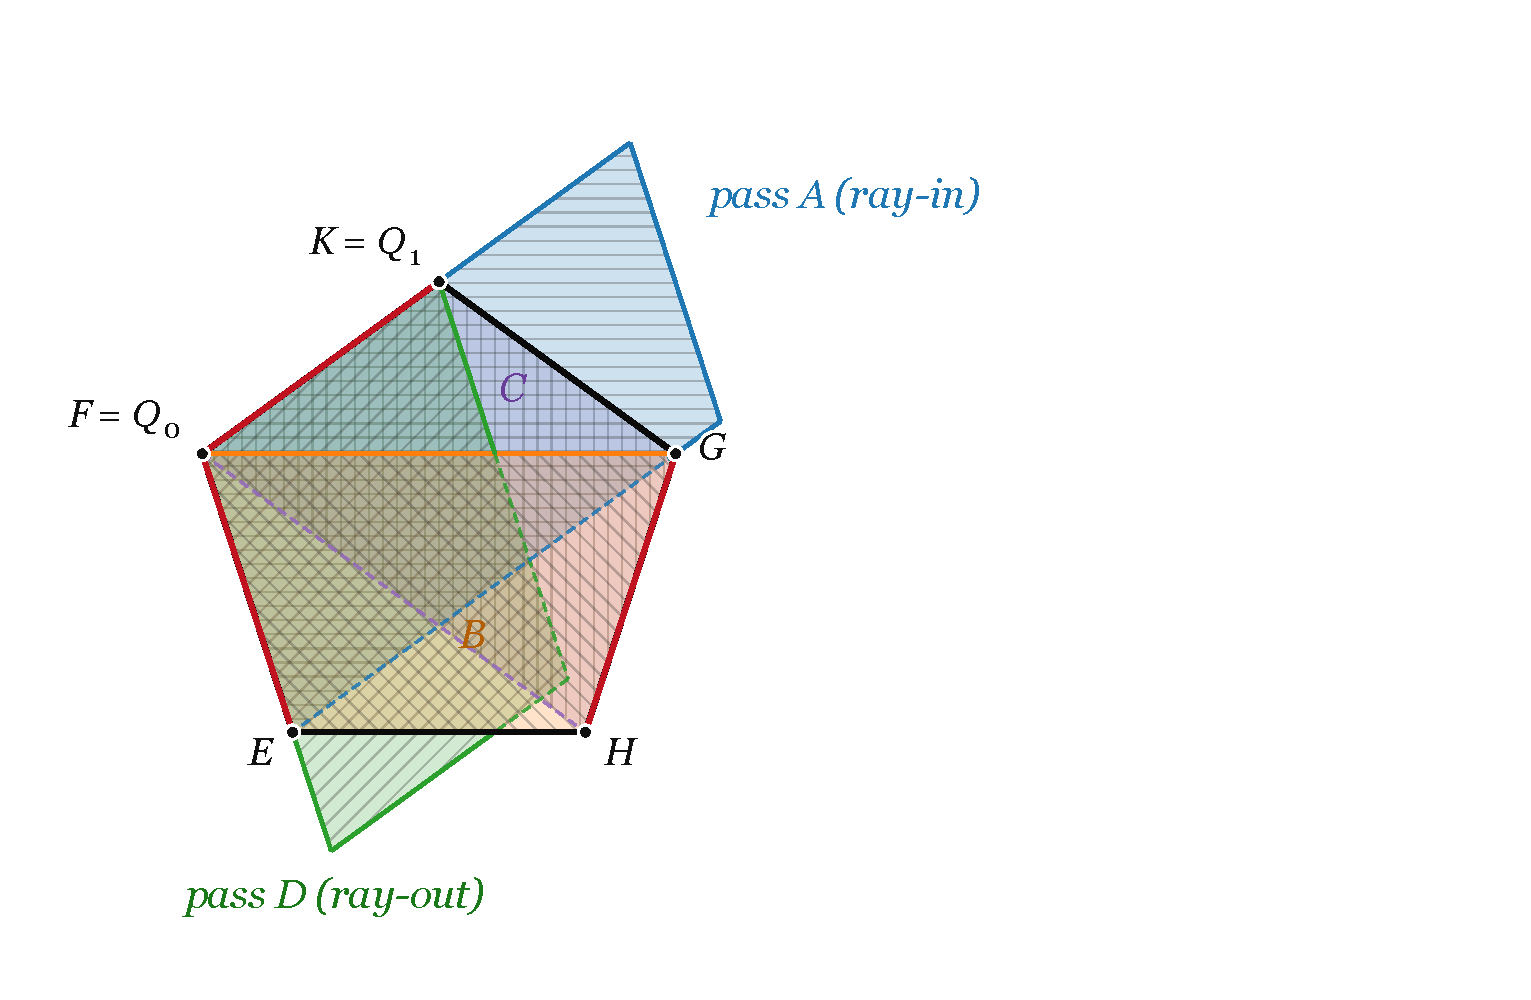
\includegraphics[width=0.92\linewidth]{figs/fig1-pentagon.pdf}
\caption{The folklore state $P^*$, drawn from the exact slice coordinates and rendered in the hidden-line convention: solid edges are visible, dashed edges pass beneath, under the layer order $B>D>A>C$. The creases are the heavy red chords, the regular pentagon $EHGKF$ is drawn in bold, and the two rays record the tying.}
\label{fig:pentagon}
\end{figure}

\subsection{Layer order, cyclic local orders, and common four-pass overlap}

\begin{definition}[Crease-neighbourhood axiom]\label{def:axiom}
If a crease $\kappa$ joins the passes $P$ and $P'$, then no neighbourhood of any point of the relative interior of $\kappa$ may be covered by a pass lying strictly between $P$ and $P'$ in the layer order.
\end{definition}

The words ``of \emph{any} point of the relative interior'' are what make the axiom bite at crease endpoints, and that is where the walls of the next subsection come from.

\begin{theorem}[Crossing relations and unique global layer order]\label{thm:layer}
In any valid flat folded state with the three-crease overhand crossing pattern, the over-under relations at the three crossings are $A>C$, $D>A$, and $B>D$ (or the global reversal). Consequently, any \emph{global} total layer order on $\{A,B,C,D\}$ compatible with these crossings is uniquely $B>D>A>C$ (up to global reversal).
\end{theorem}

\begin{proof}
By Theorem~\ref{thm:foldnumber} the three crossings sit on the non-adjacent pairs $(A,C)$, $(A,D)$ and $(B,D)$. In the material passage sequence the only freedom is the order of the two crossings inside the piece $A$ and inside the piece $D$, since $B$ and $C$ are traversed once each. Imposing alternation, that is parity of passages, together with per-crossing complementarity, namely that the two passages of one crossing have opposite parity, eliminates three of the four cases:
\begin{center}
\small
\begin{tabular}{llp{0.42\linewidth}}
\hline
order in $A$ & order in $D$ & verdict\tabularnewline
\hline
$C$ first & $A$ first & \raggedright consistent: the pairs $(1,4)$, $(2,5)$, $(3,6)$ all have opposite parity\tabularnewline
$C$ first & $B$ first & \raggedright $(A,D)$ occupies positions $(2,6)$, both even\tabularnewline
$D$ first & $A$ first & \raggedright $(A,C)$ occupies positions $(2,4)$, both even\tabularnewline
$D$ first & $B$ first & \raggedright $(A,C)$ at $(2,4)$ and $(B,D)$ at $(3,5)$\tabularnewline
\hline
\end{tabular}
\end{center}
The surviving word, with the alternating assignment, yields the three local relations $A>C$, $D>A$, and $B>D$, which are acyclic and admit a unique linear extension to a global total order on $\{A,B,C,D\}$, namely $B>D>A>C$ (or its global reversal).
\end{proof}

\begin{remark}[Cyclic local layer orders and their strong realization]\label{rem:cyclic-counterexample}
Theorem~\ref{thm:layer} does \emph{not} imply that every pointwise local layer order in the sense of Definition~\ref{def:flatstate} is induced by a global total order. Take the rational working-chart state
\[
  \theta_{\mathrm{cyc}}=\bigl(\tfrac13,\,\tfrac{301}3,\,100,\,100,\,\tfrac{302}3\bigr),
  \qquad q=\tfrac13,\quad p=-\tfrac13.
\]
Its forward directions are $(-\tfrac45,-\tfrac35),(1,0),(-\tfrac45,\tfrac35),(\tfrac7{25},-\tfrac{24}{25})$, all three turn cross products equal $\tfrac35>0$, the three centreline crossings occur at distinct transverse points in material order $\mathtt{XYZXYZ}$, and all eight walls of Section~\ref{sec:moduli} are strictly positive. Yet even the four infinite width-one support bands have no triple intersection: the minimum Euclidean distance from any pairwise band intersection to a third support band is $851/40=21.275$, and distinct pairwise overlaps along each actual pass are separated longitudinally by at least $21275/936\approx22.73$ strip widths. Retaining $A>C$, $D>A$, $B>D$ at the three crossings while assigning $A>B$ on the adjacent overlap $A\cap B$ near $\kappa_1$ gives a locally consistent pointwise layer order satisfying Definition~\ref{def:axiom}, even though combining comparisons across separated plane points yields the cycle $A>B>D>A$ (indeed all $2^3=8$ adjacent-crease choices are locally consistent, only one being globally ordered).

Moreover, this cyclic local order is strongly realizable in thin slabs: fixing passes $B,C,D$ at constant heights $2\varepsilon/3,0,\varepsilon/2$, introducing on the free incoming tail $A$ over $s\in[-25,-15]$ the smooth $C^2$ isometric height transition $z(s)=\frac\varepsilon4+\frac{3\varepsilon}4 p((s+25)/10)$ paired with horizontal arc-length parameter $S'(s)=\sqrt{1-(z'(s))^2}$ (where $p(t)=10t^3-15t^4+6t^5$, so $|z'(s)|\le\frac{9}{64}\varepsilon$ and the total horizontal foreshortening $\int_{-25}^{-15}(1-\sqrt{1-(z')^2})\,ds\le\frac{405}{2048}\varepsilon^2$ is absorbed along the free ray while all three \emph{reference flat creases} stay fixed), and joining each crease by a semicircular hairpin of radius $r$ (whose rounded material-crease midpoint projects at distance $(\pi/2-1)r$ from its reference crease, within the strong-realization tolerance) yields a strong $\varepsilon$-realization of $\theta_{\mathrm{cyc}}$ for all $0<\varepsilon\le 1/100$ with uniform projection constant $C=1$, collar constant $C_{\mathrm{ram}}=2$, sheet separation at least $\varepsilon/6$, and the same alternating trefoil knot type. The rational band separations, longitudinal overlap gaps, free-tail ramp clearance, and ramp derivative/foreshortening bounds are certified exactly in \texttt{exact\_common\_overlap}. Accordingly, the global total order $B>D>A>C$ is an explicit part of the definition of the globally ordered branch $\mathcal B$ used in Theorems~\ref{mainthm:moduli}, \ref{mainthm:realization}, and~\ref{mainthm:census}.
\end{remark}

\begin{lemma}[Common four-pass overlap forces the global order]\label{lem:common-overlap}
Suppose $(f_\theta,\lambda)$ is a flat folded state with the overhand crossing pattern and crossing relations $A>C$, $D>A$, $B>D$, whose pointwise local layer order $\lambda$ is locally constant on each pairwise pass overlap. If there exists a plane point $P$ lying strictly in the interior of all four passes $A,B,C,D$, then $\lambda$ is forced to coincide with the global total order $B>D>A>C$ on every pairwise overlap meeting $P$. This hypothesis holds:
\begin{enumerate}
\item[(i)] throughout the standard slice $0<x<1/\sqrt3$, at the point $P(x)=\bigl(\frac{h(x)}{2},\frac34\bigr)$;
\item[(ii)] at the regular pentagon $P^*$, at $\td$, on a coordinate cube of radius $10^{-3}$ around each, and along the entire certified second-family arc $[x^\dagger,x_0]$ together with its coordinate tube of radius $10^{-4}$, at the fixed point $P=\bigl(\frac12,\frac34\bigr)$.
\end{enumerate}
Consequently, the local optimality and certified-path results of Theorems~\textup{\ref{mainthm:pass}}--\textup{\ref{mainthm:kauffman}} hold under purely pointwise local layer order without assuming a global order \emph{a priori}.
\end{lemma}

\begin{proof}
Each pass image is convex, so each pairwise interior overlap $A^\circ\cap C^\circ$, $A^\circ\cap D^\circ$, $B^\circ\cap D^\circ$ is convex and hence connected. Local constancy of the relative order transports the three crossing relations $A>C$, $D>A$, $B>D$ from the three crossing points to the common interior point $P$. Because $\lambda$ is a linear order on the four material preimages over $P$, transitivity at $P$ forces $B>D>A>C$ at $P$, and local constancy on each connected pairwise overlap carries those relations to every pair overlapping at $P$.

For \textup{(i)}, evaluating the fourteen inward half-plane functionals of the four crease-bounded passes at $P(x)=(h(x)/2,3/4)$ on the standard slice \eqref{eq:slice} yields rational functions whose nontrivial numerators are $1+x^2-4x^4$, $3+6x^2-5x^4$, and $3x^2\pm2x+1$, all strictly positive on $0<x<1/\sqrt3$. For \textup{(ii)}, exact Sturm counts show that $N_5(x,1.035)$ and $N_5(x,1.053)$ have no roots on $[0.322,0.325]\supset[x^\dagger,x_0]$, confining the second-family branch to $h\in(1.035,1.053)$; outward-rounded interval evaluation of all fourteen half-plane functionals at $(1/2,3/4)$ over the $10^{-3}$ cubes around $P^*$ and $\td$ and over $192$ sub-boxes covering $[0.322,0.325]\times[1.035,1.053]$ thickened by $10^{-4}$ in all five coordinates certifies strict interior membership throughout (all interval lower bounds strictly above $0.05$, \texttt{exact\_common\_overlap}).
\end{proof}

\begin{corollary}[Prohibition lists]\label{cor:btw}
On the globally ordered branch $\mathcal B$ (with total order $B>D>A>C$), the sets of passes lying strictly between the two sides of a crease, as in Definition~\textup{\ref{def:axiom}}, are $\mathrm{Btw}(\kappa_1)=\{D\}$, $\mathrm{Btw}(\kappa_2)=\{A,D\}$ and $\mathrm{Btw}(\kappa_3)=\{A\}$.
\end{corollary}

\subsection{The walls}

Every codimension-one component of the non-penetration boundary of $\M$ is either a crease-endpoint sliver contact or a taco contact. This is not an empirical inventory but a consequence of convexity, and the following lemma is what closes it.

\begin{lemma}[Completeness of the contact catalogue]\label{lem:wallcat}
Fix a forbidden pair $(\kappa,P)$ with $P\in\mathrm{Btw}(\kappa)$, where $\kappa$ is a crease chord and $\bar P$ is the closed image of the pass, a convex polygon, possibly unbounded. Along any continuous path of states on which $\mathrm{relint}(\kappa)\cap P^\circ$ passes from empty to nonempty, the transition state satisfies, one of:
\textup{(i)} an endpoint of $\kappa$ lies on $\partial P$; or
\textup{(ii)} a vertex of $\bar P$ lies on $\kappa$.
Since every vertex of a pass image is the image of a crease endpoint, events of type \textup{(ii)} are crease-pair contacts. Consequently every codimension-one component of the non-penetration boundary is an endpoint sliver or a crease-pair contact.
\end{lemma}

\begin{proof}
At the transition state one has $\kappa\cap\bar P\ne\emptyset$, by taking a limit of intersection points from the violating side, while $\mathrm{relint}(\kappa)\cap P^\circ=\emptyset$. Pick $p\in\kappa\cap\bar P$. Suppose first $p\in\mathrm{relint}(\kappa)$; then $p\notin P^\circ$, so $p\in\partial P$. If $p$ lay in the relative interior of an edge $e$ of $\bar P$, the defining inequalities of all other edges would be strict at $p$, so near $p$ the set $\bar P$ coincides with the closed half-plane of $e$; if $\kappa$ is not parallel to $e$, it crosses the line of $e$ transversally, placing nearby relative-interior points in $P^\circ$, a contradiction. If it is parallel, the contact is collinear. The closed interval $\kappa\cap e$ then has an endpoint that is an endpoint of $\kappa$ or an endpoint of $e$ (also when $e$ is a ray or a line). These give \textup{(i)} and \textup{(ii)}, respectively. If $p$ was a vertex to begin with, \textup{(ii)} holds directly. Otherwise every point of $\kappa\cap\bar P$ is an endpoint of $\kappa$; such an endpoint cannot lie in $P^\circ$, since openness would force nearby relative-interior points of $\kappa$ into $P^\circ$, so it lies on $\partial P$, which is case \textup{(i)}.
\end{proof}

\begin{corollary}[The wall catalogue of the overhand branch]\label{cor:wallcomplete}
Within the stated working chart, the non-penetration boundary of the honest moduli $\M_{\mathrm{hon}}$ consists exactly of the six sliver walls of Table~\textup{\ref{tab:walls}} together with the windowed taco faces $\{t=1,\,0\le u\le1\}$ and $\{u=1,\,0\le t\le1\}$; the computational chamber $\Mhat$ is cut out by the same six slivers together with the unwindowed faces $\{w_9=0,\,w_{10}\le0\}$, $\{w_{10}=0,\,w_9\le0\}$ of \eqref{eq:taco}, whose extensions beyond the windows are capture faces and bound no contact.
\end{corollary}

\begin{proof}
The forbidden pairs are those of Corollary~\ref{cor:btw}, giving eight candidate endpoint events of type \textup{(i)}: both endpoints for each of $(\kappa_1,D)$, $(\kappa_2,A)$, $(\kappa_2,D)$, $(\kappa_3,A)$. Six of them are the walls of Table~\ref{tab:walls}. The remaining two, the $H$-endpoint of $\kappa_2$ against $A$ and the $G$-endpoint of $\kappa_2$ against $D$, degenerate: in the normalization \eqref{eq:coords}, with $d_2=((x^2-1),-2x)/(1+x^2)$, the band containing $A$ satisfies $0\le\operatorname{cross}(P-E,d_2)\le1$, whereas $\operatorname{cross}(H-E,d_2)=-2hx/(1+x^2)<0$. Thus $H$ is strictly outside this band on the positive chart, rather than on its carrier line. Material reversal gives the analogous strict exclusion of $G$ from the band of $D$. Adjacent crease contacts are excluded by the positive material chord distance of the intervening panel (Proposition~\ref{prop:axred}). Events of type \textup{(ii)} are crease-pair contacts; adjacent pairs are excluded by the same distance argument, leaving the pair $(\kappa_1,\kappa_3)$, whose codimension-one events are endpoint-on-segment incidences of the two crease segments. Two of the four, $F\in\kappa_3$ and $Q_0\in\kappa_1$, are exactly the taco faces $\{w_9=0,\,w_{10}\le0\}$ and $\{w_{10}=0,\,w_9\le0\}$ of \eqref{eq:taco}, by Observation~\ref{obs:corner}; the remaining two, $E\in\kappa_3$ and $Q_1\in\kappa_1$, never occur on the chart, by Lemma~\ref{lem:tacoent}(ii).
\end{proof}

With the sign convention that the feasible side is $\ge0$, the six sliver walls are those of Table~\ref{tab:walls};\footnote{The numbering is inherited from a longer preliminary list; the conditions originally labelled $w_2,w_3$ proved to be consequences of the others and are not walls. We keep the labels to stay aligned with the ancillary material.} each is the analytic statement that a particular pass fails to cover a neighbourhood of a particular crease endpoint. Because these conditions concern the endpoints of a relative interior, they must be evaluated analytically and never by sampling along the crease; see Remark~\ref{rem:methods}.

\begin{table}[t]
\centering\small
\begin{tabular}{lp{0.28\linewidth}p{0.42\linewidth}}
\hline
wall & \raggedright analytic meaning & \raggedright event forbidden by Definition~\ref{def:axiom}\tabularnewline
\hline
$w_1$ & \raggedright endpoint $G$ of $\kappa_2$ inside the lay-in band & \raggedright $A$ covers the $G$-side sliver of $\kappa_2$\tabularnewline
$w_4$ & \raggedright endpoint $H$ of $\kappa_2$ inside the lay-out band & \raggedright $D$ covers the $H$-side sliver of $\kappa_2$\tabularnewline
$w_5$ & \raggedright $\Delta\ge0$: $K$ at or beyond $I$ along $r$ on $\ell_2$ & \raggedright $A$ covers a neighbourhood of $\kappa_3$\tabularnewline
$w_6$ & \raggedright the mirror of $w_5$ & \raggedright $D$ covers a neighbourhood of $\kappa_1$\tabularnewline
$w_7$ & \raggedright $Q_0$ not beyond the far edge $e_B$ of the lay-in band & \raggedright $A$ covers the $Q_0$-side sliver of $\kappa_3$\tabularnewline
$w_8$ & \raggedright $F$ not beyond the far edge of the lay-out band & \raggedright $D$ covers the $F$-side sliver of $\kappa_1$\tabularnewline
\hline
\end{tabular}
\caption{The six endpoint-sliver walls of $\M$ in the normalization \eqref{eq:coords}. Each is a corner-on-edge contact, a crease endpoint of one pass meeting the boundary of another.}
\label{tab:walls}
\end{table}

The remaining boundary has a different logical shape. Let $E+t(F-E)=Q_1+u(Q_0-Q_1)$ be the intersection of the \emph{lines} carrying $\kappa_1$ and $\kappa_3$, and set $w_9=t-1$ and $w_{10}=u-1$. The forbidden event is that the two crease \emph{segments} cross in their relative interiors---the taco--taco prohibition of flat origami \cite{justin1997}---that is
\[0<t<1\quad\text{and}\quad 0<u<1\quad\text{simultaneously}.\]
The lower bounds are not additional walls: they are governed by an exact linear entanglement of the pair.

\begin{lemma}[Entanglement of the taco pair]\label{lem:tacoent}
Write $q=g-h$, $W_0=(1+q^2)w_0=(q^2-1,2q)$, $\alpha=2aq/(q^2+1)$ and $\beta=2bq/(q^2+1)$, so that the endpoints of $\kappa_3$ sit at heights $y(Q_1)=1+\alpha$ and $y(Q_0)=\beta$. On the chart, where $h,a,q>0$:
\begin{enumerate}
\item the identity $t-1=\alpha(1-u)+u\,(\beta-1)$ holds, the height along the line of $\kappa_3$ taking the value $t$ at the intersection point;
\item the endpoint events $E\in\kappa_3$ and $Q_1\in\kappa_1$ never occur: $\kappa_3$ lies in the closed band of $C$, whose $H$-side edge line has $E$ strictly on its far side, by $\operatorname{cross}(E-H,W_0)=-2hq<0$ against the band-side value $\operatorname{cross}(G-H,W_0)=q^2+1>0$; and $y(Q_1)=1+\alpha>1\ge\max_{\kappa_1}y$;
\item on $\{\beta\ge1\}$ the forbidden event is impossible: $0<u<1$ forces $t-1=\alpha(1-u)+u(\beta-1)>0$;
\item $\beta\equiv1$ on the standard slice, where $Q_0=F$ identically; on the certified segment of the second family from $P^*$ to $\td$, one has $\beta>1$ away from $P^*$ and $1+\alpha-\beta>0$ throughout, by root-free resultants with $N_5$ and exact sign anchors, the pentagon endpoint factor of $\beta-1$ deflating exactly; at $P^*$, $\beta=1$ and $\alpha=(\sqrt5-1)/2=\varphi^{-1}$; at $\td$, $t-1=u-1\approx0.0506$ and $\beta-1\approx0.0796$, both certified positive in $\Q[x]/(p_x)$; and along this segment $t=u=(1+x^2-2hx)/(4x^2)$ in closed form. Certificate \texttt{exact\_taco} \cite{anc}.
\end{enumerate}
\end{lemma}

On $\{t>0\}\cap\{u>0\}$ the complement of the forbidden event is therefore exactly the union
\begin{equation}\label{eq:taco}
  \{w_9\ge0\}\cup\{w_{10}\ge0\},
\end{equation}
while on $\{t\le0\}\cup\{u\le0\}$ the prohibition is vacuous and \eqref{eq:taco} is a strengthening. Three spaces organize the discussion. $\Mhon$ is the moduli with the honest prohibition. $\Mplus:=\Mhon\cap\{t>0,\,u>0\}$ is the \emph{positive-taco moduli}, on which the honest prohibition coincides exactly with the disjunction \eqref{eq:taco}. $\Mhat$ is the \emph{computational chamber}: the semialgebraic set cut out by the sliver walls and the unwindowed disjunction \eqref{eq:taco}, with no positivity requirement on $(t,u)$. Then
\[\Mplus\;=\;\Mhat\cap\{t>0,\,u>0\}\;\subseteq\;\Mhat\;\subseteq\;\Mhon,\]
the second inclusion because \eqref{eq:taco} implies the honest prohibition outright. Every state at which this paper runs a first- or second-order analysis---the standard slice, both one-parameter families, $P^*$, and $\td$---lies in $\Mplus$ with margins certified by Lemma~\ref{lem:tacoent}(iv), and near those states the three spaces agree: the far pieces $\{t\le0\}\cup\{u\le0\}$ are empty in a neighbourhood, so \eqref{eq:taco} \emph{is} the segment-crossing prohibition there. Throughout, the working symbol $\M$ denotes the chamber $\Mhat$: every existence, reachability, and path statement proved in $\M$ holds verbatim in $\Mhon$, the local theorems may be read in $\Mplus$ unchanged, and the census of Section~\ref{sec:census} runs over $\Mhat$, whose faces beyond the windows are \emph{capture faces}---constraint extensions, not non-penetration walls. The stratified census of Section~\ref{sec:census} is likewise unaffected: its recorded exclusion verdicts rest on sliver-wall signs and Krawczyk isolation alone, never on the taco pair. The honest catalogue is also settled by the same lemma: a path of honest states entering the forbidden box must cross its boundary, the entry faces $\{t=0,\,0\le u\le1\}$ and $\{u=0,\,0\le t\le1\}$ are empty by Lemma~\ref{lem:tacoent}(ii), so the honest non-penetration boundary consists of the six slivers together with the \emph{windowed} taco faces $\{t=1,\,0\le u\le1\}$ and $\{u=1,\,0\le t\le1\}$; the chamber's faces extend these beyond the windows, and the extensions $\{t=1,\,u<0\}$, $\{u=1,\,t<0\}$ separate two honestly-valid regions and bound no contact. The union \eqref{eq:taco} is not convex. We call $w_9,w_{10}$ the \emph{taco pair}: the forbidden event is two creases folding shut on one another. First-order blocking tests must therefore be run separately on the two branches $\{w_1,\dots,w_8,w_9\}$ and $\{w_1,\dots,w_8,w_{10}\}$; on each branch the constraint system is an ordinary linear one, and Carath\'eodory's theorem makes the enumeration of basic solutions a complete decision procedure \cite{barvinok2002,nocedal2006}.

\begin{observation}[The taco walls are corner contacts]\label{obs:corner}
One has $w_9=w_{10}=0$ if and only if $Q_0=F$. Indeed $t=1$ places the intersection of the two crease lines at $F$ and $u=1$ places it at $Q_0$. The locus $\mathcal F=\{Q_0=F\}$ is cut out by two equations and is a three-dimensional submanifold of $\M$; its intersection with $\{w_1=w_4=0\}$ is exactly the standard slice, on which all six of $w_1,w_4,w_7,w_8,w_9,w_{10}$ vanish identically. The taco pair is thus not a self-intersection of a pass but a corner contact of the crease pair $\kappa_1,\kappa_3$.
\end{observation}

\begin{proposition}[Stratification]\label{prop:strat}
Inside the fixed nondegenerate branch chart, the relative closure of $\M$ is semialgebraic and is stratified by the active constraint set; the full closure in $\R^5$ acquires, in addition, code and general-position degeneration faces---branch-exit events, open conditions in the branch datum, not part of the wall stratification. The standard slice is exactly $\{w_1=w_4=w_7=w_8=0\}$, the four contact equations of the classical slice construction being equivalent to the activation of these four walls, and the regular pentagon is the unique point at which all eight walls, sliver and taco alike, are active. Two further contact functions, incidence of $F$ with an edge and passage of $\kappa_3$ through $F$, are not walls but stratum labels, since both signs occur among valid states.
\end{proposition}

\begin{proof}
Semialgebraicity is immediate, every wall function being rational with integer-coefficient numerator and denominator; denominators are nonzero with fixed signs on each chart component. The identification of the standard slice with $\{w_1=w_4=w_7=w_8=0\}$, the simultaneous activity of all eight sliver and taco walls at the regular pentagon and at no other point, and the occurrence of both signs of the two discarded contact functions are direct computations, verified in exact arithmetic in the ancillary suite \cite{anc}.
\end{proof}

\begin{proposition}[Axiom reduction]\label{prop:axred}
On the globally ordered overhand branch $\mathcal B$, the crossing datum determines the unique global layer order $B>D>A>C$ \textup{(Theorem~\ref{thm:layer})}, and that global order together with Definition~\textup{\ref{def:axiom}} implies the transversality clause of crease-pair non-crossing. Hence within $\mathcal B$ the only logically independent axioms are the crease-neighbourhood axiom and the branch datum (including the global layer order).
\end{proposition}

\begin{proof}
Adjacent crease pairs cannot meet at all, since the distances $d(\kappa_1,\kappa_2)$ and $d(\kappa_2,\kappa_3)$ equal the corresponding material chord distances, which are positive by rigidity of the intervening panel. If $\kappa_1$ and $\kappa_3$ crossed transversally in their relative interiors, then a relative interior point of $\kappa_1$ next to the crossing would lie in the interior of the image of $D$, and $D\in\mathrm{Btw}(\kappa_1)$ by Corollary~\ref{cor:btw}, violating Definition~\ref{def:axiom}. Collinear overlap of two creases is not covered by this argument, since in that degenerate case $D$ covers only a half-neighbourhood; it is excluded here by the explicit nonparallel-crease condition of the working chart, not by centreline general position. No conclusion for parallel crease pairs follows from this argument.
\end{proof}

Proposition~\ref{prop:dim}, Theorem~\ref{thm:layer}, Lemma~\ref{lem:wallcat}, Corollary~\ref{cor:wallcomplete}, Observation~\ref{obs:corner} and Propositions~\ref{prop:strat} and~\ref{prop:axred} together constitute Theorem~\ref{mainthm:moduli}.

\begin{remark}[Status of the classification]\label{rem:wallsnum}
Lemma~\ref{lem:wallcat} and Corollary~\ref{cor:wallcomplete} give the complete wall list. Exact witnesses of both signs show that the two stratum labels of Proposition~\ref{prop:strat} bound no face. The ancillary material \cite{anc} includes these witnesses, the endpoint criteria and supplementary numerical boundary sweeps.
\end{remark}

\section{Tightening and the pentagonal junction}\label{sec:tightening}

\subsection{The functional of pulling}

\begin{definition}[Core length]\label{def:core}
Let $m_1<\cdots<m_n$ be the material points at which the centreline meets the creases and let $M_i$ be their images. The \emph{core length} is
\[
  \core=m_n-m_1=\sum_{i=1}^{n-1}|M_iM_{i+1}| ,
\]
the material trapped between the first and the last crease; the second equality holds because panels are rigid.
\end{definition}

\begin{proposition}[Why this is the functional of pulling]\label{prop:pulling}
On a finite strip of length $L$ the two tails have total material length $L-\core$. Hence extracting as much tail as possible and minimizing $\core$ are the same problem, and only the latter survives the passage to long strips.
\end{proposition}

This is where the model parts company with Kauffman's truncation length $\trunc$ \cite{kauffman2004}, which measures the material needed to \emph{build} the flat knot rather than the material that pulling extracts. Both are natural, both are defined on the same moduli space, and the sequel shows that they select different strict local optima.

\begin{definition}[Pulling path and tight state]\label{def:pull}
A \emph{pulling path} is a continuous path $p\colon[0,1]\to\overline{\M}$ which satisfies non-penetration at all times while preserving the branch, so that crumpling and layer rearrangement are excluded by definition, and along which $\core\circ p$ is non-increasing. A state reachable from a slack state, one at which all contact inequalities are strict, is \emph{tight} if no pulling path issuing from it strictly decreases $\core$.
\end{definition}

This is the path version of a constrained local minimum. It combines the contact-force characterization familiar from ropelength criticality \cite{cks2002,svdm2004} with the monotone-path formulation used for expansive motions \cite{cdr2003}; the balance between the gradient of the objective and the active wall gradients that appears below is the folded analogue of the vertex tension balance of the immersed theory \cite{immersed2020,ayala2025}.

\subsection{The slice theorem}

\begin{lemma}[Closed form on the slice]\label{lem:sliceform}
On the standard slice the two core segments have equal length and
\[
\begin{gathered}
  |M_1M_2|=|M_2M_3|=\frac{1-x^2}{2x},\qquad
  \core(x)=\frac{1-x^2}{x}=\frac1x-x,\\
  \core'(x)=-\frac1{x^2}-1<0 .
\end{gathered}
\]
Pulling along the slice is therefore exactly the increase of $x$.
\end{lemma}

\begin{proof}
The end exchange of the slice swaps the two core segments, so they have equal length. Substituting the values of $g$ and $h$ from \eqref{eq:slice} into $(g+h+x)/2$, the common length of the two segments, gives $(1-x^2)/(2x)$; summing and differentiating gives the remaining two identities. The computation is verified in exact arithmetic in the ancillary suite \cite{anc}.
\end{proof}

\begin{theorem}[Slice tightening]\label{thm:slice}
A pulling path confined to the standard slice $\{x\in(0,\tfrac1{\sqrt3})\}$ has feasible region $\{\Delta(x)\ge0\}=(0,x_0]$ and a unique tight state, at $x=x_0=\sqrt{1-2/\sqrt5}$: the regular pentagon.
\end{theorem}

\begin{proof}
The slice is one-dimensional with parameter $x$ by Proposition~\ref{prop:strat}. The gap $\Delta=k-\mu$ of \eqref{eq:slice} is strictly decreasing with a unique zero $x_0$ in $(0,\tfrac1{\sqrt3})$; strict decrease follows from the sum-of-squares identity
\[
  5x^6-5x^4+7x^2+1=5x^2\Bigl(x^2-\tfrac12\Bigr)^2+\tfrac{23}4x^2+1>0
\]
for the numerator of $\Delta'$. Since $\core$ is strictly decreasing by Lemma~\ref{lem:sliceform}, a pulling path can only increase $x$, and at $x_0$ the wall $w_5$, that is $\Delta=0$, equivalently $K=I$, equivalently $\kappa_3$ flush with the far edge $e_B$, becomes active. For $x<x_0$ a further increase is possible, so no earlier point is tight.
\end{proof}

At $x_0$ all five sides of the central polygon $E,H,G,K,F$ have equal length, with $|EH|^2=2-\tfrac{2\sqrt5}5$, all five interior angles have cosine $-\tfrac{\sqrt5-1}4=\cos108^\circ$, and the two tails make an angle of $72^\circ$. These are exact identities in $\Q(\sqrt5)$, checked by the symbolic geometry scripts. Lean~4 checks supporting algebraic identities, including $|EH|^2=|EF|^2$ under the contact equation and a positivity identity proving the monotonicity of $\Delta$; it does not formalize the polygon or its five angles \cite{mathlib2020,anc}. The five sides are precisely the three creases and two band edges: the pentagon is not an approximation but the exact contact-limited endpoint of the slice, which is the folklore statement, proved.

\subsection{Tightening cannot stop in the interior}

\begin{proposition}[Affine core length and no interior critical point]\label{prop:nointerior}
On the forward chart, where $g+h+x>0$ and $a+b>0$,
\[
  \core(\theta)=\frac{x+g+h+a+b}{2},\qquad
  \nabla\core=\tfrac12\mathbf1,\qquad \nabla^2\core=0.
\]
In particular there is no interior critical point.
\end{proposition}

\begin{proof}
An isometry takes the midpoint of a complete material crease chord to its centreline fold point. Thus
$M_1=(-x/2,1/2)$, $M_2=((g+h)/2,1/2)$, and
\[
M_3=\frac{Q_1+Q_0}{2}=M_2+\frac{a+b}{2}\,w_0.
\]
Since $|w_0|=1$, the two forward centreline segments have lengths $(g+h+x)/2$ and $(a+b)/2$. Adding and differentiating proves the claim. Without the forward assumptions the respective absolute values are required. The identity and derivative are also checked by \texttt{exact\_core\_descent}.
\end{proof}

\begin{proposition}[The gradient at the pentagon]\label{prop:gradpent}
At $P^*$, as everywhere in the forward chart, $\nabla\core=\tfrac12\mathbf1$. The equality of its five entries is a consequence of complete-chord midpoint geometry, not a special symmetry of the pentagon.
\end{proposition}
\begin{proof}
Apply Proposition~\ref{prop:nointerior}.
\end{proof}

\subsection{The pentagon is a contact-mode junction: descent passes through}

The term is descriptive; no minimax theory is invoked.

\begin{theorem}[The pentagonal contact-mode junction: descent passes through $P^*$]\label{thm:pass}
At $P^*$ all eight walls are active. For each of the two taco branches of \eqref{eq:taco} the gradient $\nabla\core$ does \emph{not} lie in the non-negative cone spanned by the active wall gradients: every basic solution has a negative multiplier, and by Carath\'eodory's theorem the test is complete. Consequently a first-order feasible descent direction exists; explicitly,
\[
  \delta^*\approx(-0.0844,\ +0.4420,\ -0.5786,\ -0.5786,\ +0.3576)
\]
keeps $w_1=w_4=w_5=w_6=0$ to first order, moves $w_7,w_8,w_9,w_{10}$ into the feasible side, and satisfies $\nabla\core\cdot\delta^*<0$. There is also a strictly inward rational descent direction
\begin{gather*}
d=10^{-6}(-163127,1000000,-883304,-887250,833681),\\
\nabla\core\cdot d=-\frac1{20}.
\end{gather*}
Every one of the eight wall derivatives is strictly positive along $d$; the first four lie between $0.0857$ and $0.0858$, and the last four between $3.199$ and $3.204$. Hence $P^*+td$ is feasible with decreasing core length for all sufficiently small $t>0$. The regular pentagon is therefore not a local minimum of $\core$.
\end{theorem}

\begin{proof}
All wall functions and $\core$ are rational in $\theta$, since reflections preserve norms and no normalization is required, so every gradient at $P^*$ is an exact element of $\Q(\sqrt5,x_0)$. The Farkas alternative is decided exactly on each branch by \texttt{exact\_farkas2}, and $\delta^*$ is a rounding of the exact solution of the four-equality system. Independently, \texttt{exact\_core\_descent} encloses each derivative along the displayed rational $d$ strictly above zero. Taylor expansion makes all eight active walls positive for small $t>0$, while the open branch conditions persist by continuity. The affine core formula makes its decrease exactly $t/20$. This supplies a nonlinear feasible path, rather than relying on tangency alone.
\end{proof}

\begin{figure}[t]
\centering
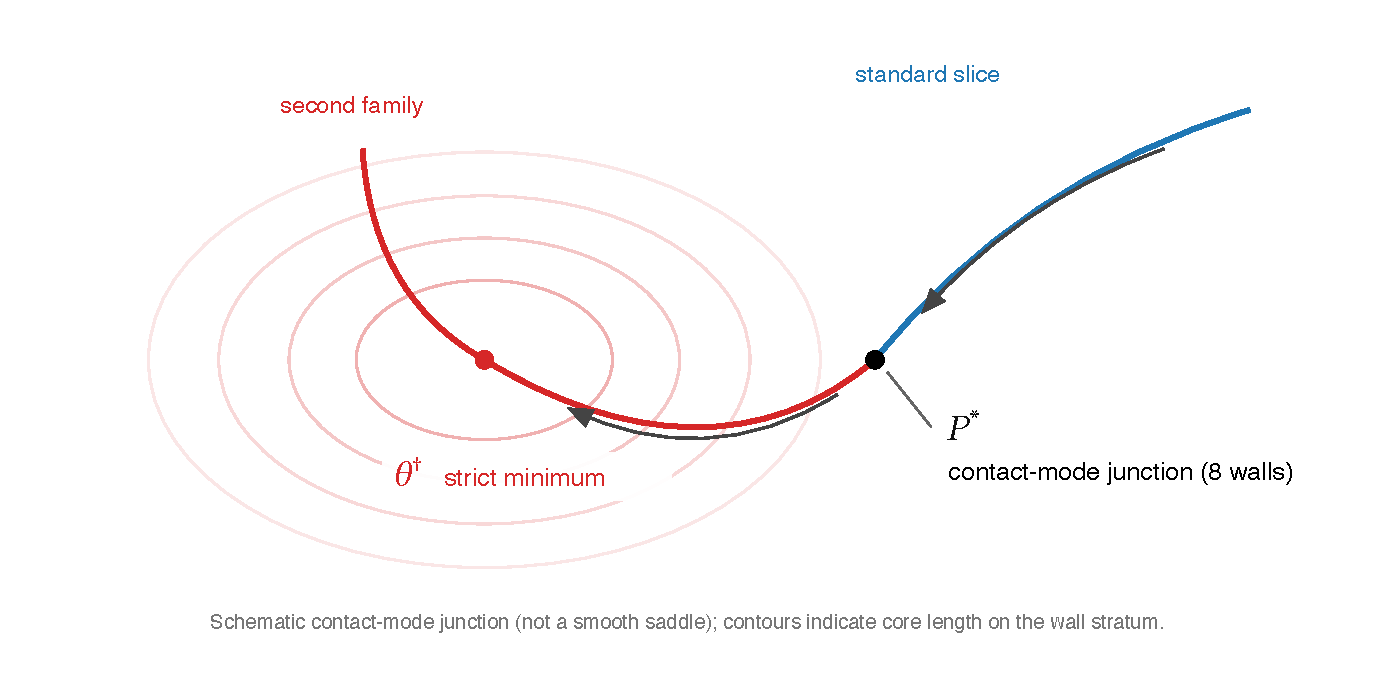
\includegraphics[width=0.92\linewidth]{figs/fig3-mountain-pass.pdf}
\caption{The regular pentagon as a contact-mode junction---informally, a mountain pass---shown schematically. The standard slice and the second symmetric family cross at $P^*$; descent of the core length passes through the crossing and continues along the second family to $\td$, feasibly and strictly monotonically by the certificates of Remark~\ref{rem:edge}.}
\label{fig:pass}
\end{figure}

\begin{proposition}[The two families and the pass]\label{prop:families}
The edge $\{w_1=w_4=w_5=w_6=0\}$ is a second mirror-symmetric one-parameter family of feasible states, the mirror symmetry surviving along it in the form $h=a$, $w_7=w_8$ and $w_9=w_{10}$, and it is distinct from the standard slice $\{w_1=w_4=w_7=w_8=0\}$. It is feasible only for $x<x_0$, since $w_7,\dots,w_{10}$ all become negative for $x>x_0$. Hence the pentagon is a common endpoint of these two distinct mirror-symmetric one-parameter families, the ones arising from the two specified symmetric active-set loci.
\end{proposition}

\begin{proof}
That the four equations cut out a one-parameter family, that the mirror symmetry survives along it in the stated form, and that the family is distinct from the standard slice are direct computations, verified in exact arithmetic in the ancillary suite \cite{anc}; the one-sided feasibility is now exact, by the certificates of Remark~\ref{rem:edge}.
\end{proof}

Geometrically, along the second family the knot releases the corner lock at $F$ and at its mirror image, so that $w_7,w_9>0$ and $w_8,w_{10}>0$, while it retains the two corner slivers $w_1,w_4$ and the two flush contacts $w_5,w_6$, and it tightens further. Theorem~\ref{thm:slice}, Theorem~\ref{thm:pass}, Proposition~\ref{prop:families} and Remark~\ref{rem:edge} together constitute Theorem~\ref{mainthm:pass}, and they turn the tightening story into a chain: the standard slice carries the classical relative tightening path inside its contact stratum, terminating at the regular pentagon, while genuine slack states reach $P^*$ along the reverse of the opening segment of Corollary~\ref{cor:slackstart}; the pentagon is passed through rather than stopped at; and descent continues along the second family to the state $\td$ analysed in the next section. Figures~\ref{fig:pass} and \ref{fig:families} display the two families and their crossing.

\begin{figure}[t]
\centering
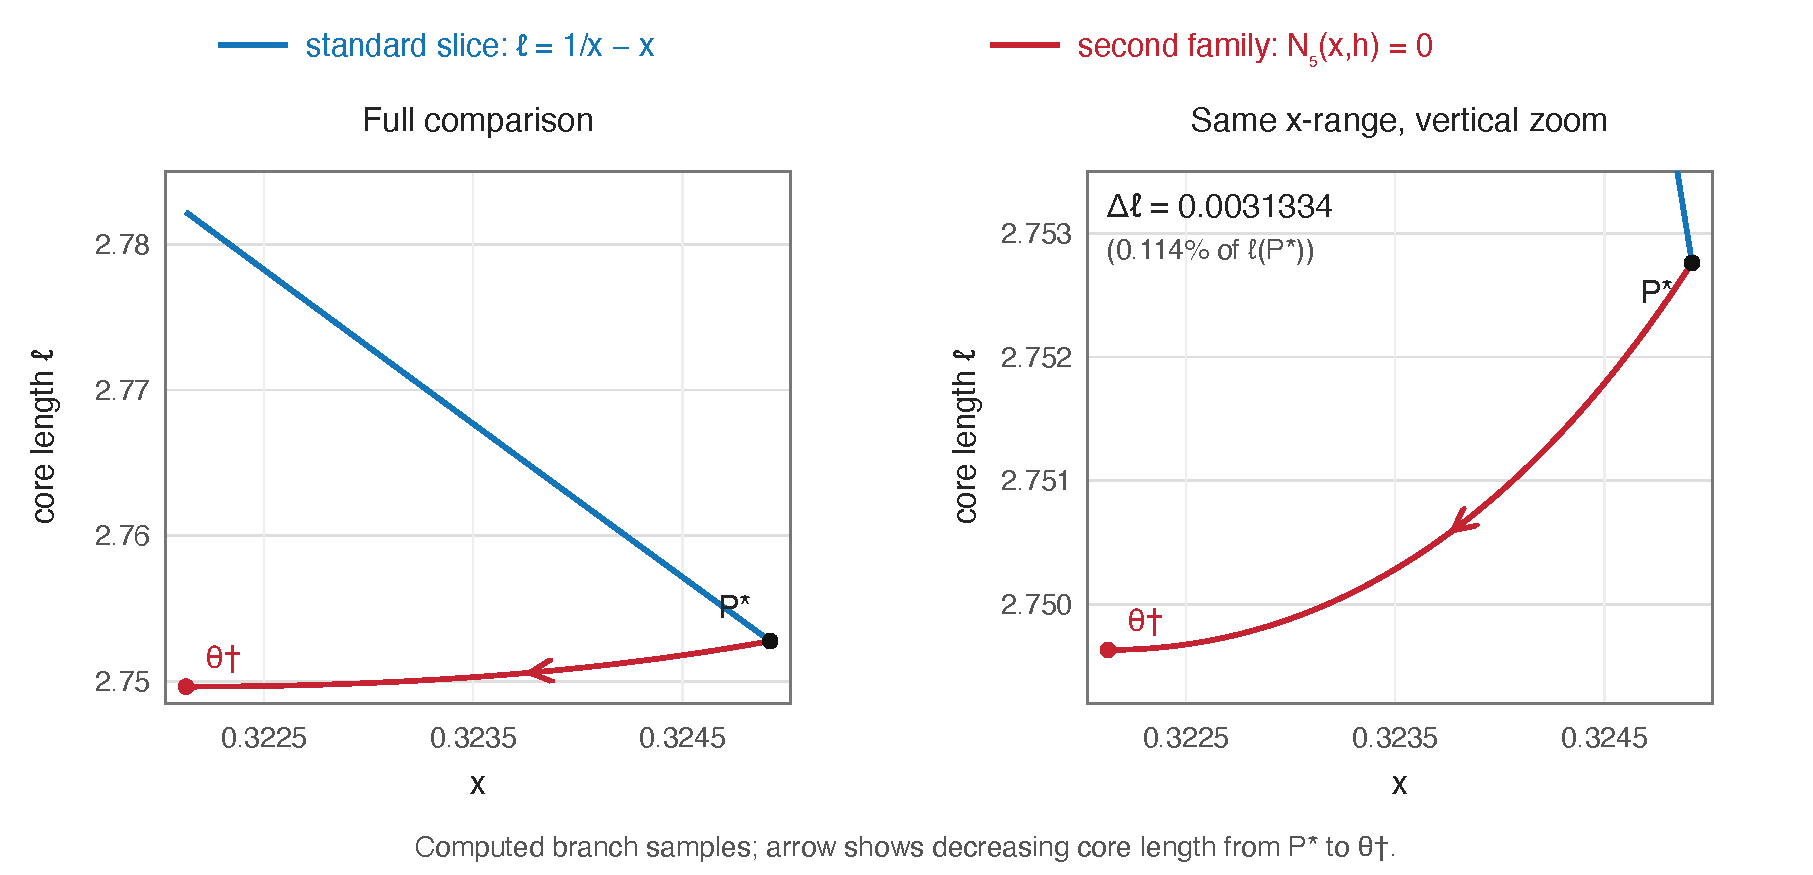
\includegraphics[width=0.92\linewidth]{figs/fig4-two-families.pdf}
\caption{The two one-parameter families in the $(x,\core)$ plane. The standard slice $\core=1/x-x$ meets the second family at $P^*$, and the second family attains its strict minimum at $\td$, below the pentagon value. Right: the same interval with an expanded vertical scale.}
\label{fig:families}
\end{figure}

\begin{remark}[Feasible monotone descent, exactly]\label{rem:edge}
Restrict the four remaining constraints to the second family. With $g$ and $b$ eliminated and $a$ replaced by $h$, each of $w_7=w_8$ and $w_9=w_{10}$ (equal in pairs, because the family lies in the mirror-fixed locus and the mirror exchanges the pairs) has a polynomial numerator in $(x,h)$ over positive denominators, and $d\core/dx$ has numerator $-K$, with $K$ the critical polynomial \eqref{eq:critpoly}, over $2x^2\,\partial_hN_5$. Exact endpoint identities hold: $K(x^\dagger,h^\dagger)\equiv0$ in $\Q[x]/(p_x)$, and at the pentagon, where $h_0^2=1+x_0^2$, the numerators of $w_7$ and $w_9$ vanish in $\Q[x]/(5x^4-10x^2+1)$. The resultants with $N_5$ of all five relevant polynomials---the two wall numerators, the taco denominator, $K$, and $\partial_hN_5$---have no real roots in $[0.322,0.325]\supset[x^\dagger,x_0]$ after removing the endpoint factors, by exact Sturm counts; the height strip of Lemma~\ref{lem:common-overlap} contains exactly one root at $x=1293/4000$, and interval Newton maps a radius-$10^{-20}$ box there strictly into its interior. The wall numerators and the taco denominator are positive at this anchor. Both $-K$ and $\partial_h N_5$ are negative, giving a positive derivative. Hence on the open interval the branch is smooth, $w_7=w_8>0$ and $w_9=w_{10}>0$, and $d\core/dx>0$ with equality only at $x^\dagger$. Descent from the pentagon along the second family therefore reaches $\td$ through valid states with strictly decreasing $\core$; the path is moreover branch-preserving, twenty-two further root-free resultants fixing the crossing pattern, passage word, and general-position margins along the whole family (Remark~\ref{rem:branchaudit}). Hence $\td$ is reachable and tight in the sense of Definition~\ref{def:pull}. The certificates are \texttt{exact\_reach} and \texttt{exact\_branch} in the ancillary suite \cite{anc}.
\end{remark}

\begin{remark}[Methods: why the certificates must be exact]\label{rem:methods}
At a sampled asymmetric state with $\core=2.6233$, the lay-in band covers a sliver of $\kappa_2$ near crease parameter $0.98$. An interior sampling grid misses the penetration, while the endpoint wall functions give $w_1=-0.061$ and $w_4=-0.062$. A second example concerns the opposite inference. A search over $400\,000$ random directions at $P^*$ found no feasible decrease. Yet the direction $d$ of Theorem~\ref{thm:pass} decreases $\core$ strictly and has positive margins on all eight walls. Its strict margins give an open cone of feasible descent directions. The tangent $\delta^*$ preserves four equalities.
\end{remark}

\section{The second family and the tight state \texorpdfstring{$\td$}{}}\label{sec:family}

Theorem~\ref{thm:pass} leaves the pulling problem in an unusual position. At the regular pentagon the gradient of the core length is the exact vector $\nabla\core=\frac12\mathbf1$ of Proposition~\ref{prop:gradpent}, and it lies in no subcone of the active wall gradients in either taco branch; the direction that certifies this keeps the four walls $w_1,w_4,w_5,w_6$ at equality while opening $w_7,w_8,w_9,w_{10}$ into the feasible side. Pulling therefore does not stop at the folklore state: it continues along the locus on which those four equalities persist,
\begin{equation}\label{eq:family}
  \mathcal E=\bigl\{\theta\in\overline{\M}\ :\ w_1(\theta)=w_4(\theta)=w_5(\theta)=w_6(\theta)=0\bigr\},
\end{equation}
the second mirror-symmetric one-parameter family of Proposition~\ref{prop:families}. This section follows $\mathcal E$ to its end.

The outcome is a single point $\td$, and every quantity associated with it is algebraic over one number field: its coordinates, the multipliers that block further pulling, and the curvature that makes the block strict all lie in a degree-twelve extension of $\Q$, so the entire optimality analysis can be carried out by exact arithmetic rather than approximation. At the same time, the field is not solvable by radicals: the splitting field of the defining sextic for $(x^\dagger)^2$ has Galois group $S_6$, so the tight state of Definition~\ref{def:pull} admits no radical expression, its $x$-coordinate already having none.

\subsection{Reduction to a plane curve}

\begin{proposition}[Family reduction]\label{prop:familyreduction}
On the mirror-symmetric component of $\mathcal E$ through $P^*$ and $\td$, the coordinates satisfy the identities
\begin{equation}\label{eq:familyids}
  g=\frac{1-x^2}{2x},\qquad a=h,\qquad b=g+x=\frac{x^2+1}{2x},\qquad \core=g+h+x=h+b,
\end{equation}
and the residual relation between the two remaining coordinates is the plane algebraic curve
\begin{equation}\label{eq:n5}
  N_5(x,h)=8h^3x^3+4h^2x^4+4h^2x^2+2hx^5-4hx^3-6hx+x^6+3x^4+3x^2+1=0 .
\end{equation}
Consequently this geometric family is represented by the selected real branch of $\{N_5=0\}$ with the positive chart and feasibility conditions retained, and on it the objective becomes a single-variable function: we abbreviate $\ell(x):=\core(c(x))$ for the restriction of the core length to the family curve $c(x)=\bigl(x,g(x),h(x),h(x),b(x)\bigr)$, so that
\begin{equation}\label{eq:ellofx}
  \ell(x)=h(x)+\frac{x^2+1}{2x} .
\end{equation}
\end{proposition}

\begin{proof}
The first wall admits the exact polynomial representative $2gx+x^2-1$, a positive multiple of $w_1$ on the branch, so for $x>0$ the equation $w_1=0$ is equivalent to $g=(1-x^2)/(2x)$. The mirror symmetry recorded in Proposition~\ref{prop:families} survives along $\mathcal E$ and identifies $a$ with $h$; it also exchanges the two core segments, so they have equal length. Since $M_1=(-x/2,\frac12)$ and $M_2=(\frac{g+h}2,\frac12)$ lie on a common horizontal line, the first core segment has length $(g+h+x)/2$ by Proposition~\ref{prop:nointerior}, whence $\core=g+h+x$. Eliminating the reflected data from the two remaining wall equations---a sequence of polynomial divisions verified by exact arithmetic in the ancillary suite \cite{anc}---leaves the identity $b=g+x$, which turns $\core=g+h+x$ into $\core=h+b$ and, with the value of $g$ already found, into $b=(x^2+1)/(2x)$; and it leaves exactly one further relation between $x$ and $h$, namely \eqref{eq:n5}.
\end{proof}

\begin{proposition}[Irreducibility of the family curve]\label{prop:n5irred}
The polynomial $N_5$ is irreducible over $\Q$. Polynomial identities established modulo $N_5$ therefore hold on its algebraic zero set; rational identities also require nonzero denominators. This does not identify all real points of that curve with valid folded states. We use only the real branch through $(x^\dagger,h^\dagger)$ and the pentagon, isolated in a rational height interval at an interior point and continued over $[x^\dagger,x_0]$ by the root-free certificates in Remark~\ref{rem:edge}.
\end{proposition}

\begin{proof}
Irreducibility is a finite computation with integer coefficients, verified by exact arithmetic in the ancillary suite \cite{anc}. The quotient $\Q[x,h]/(N_5)$ is then a domain. Remainder-zero computations establish the stated algebraic identities, while the interval and resultant certificates separately select the real branch and retain its geometric inequalities. Irreducibility alone says nothing about uniqueness of the real ordinate: at $x=1/5$, for example, the cubic $N_5(x,h)$ has three real roots.
\end{proof}

\subsection{Existence and exact identification}

\begin{proposition}[Elimination]\label{prop:elimination}
Set
\begin{equation}\label{eq:critpoly}
  K(x,h)=2x^2\,\partial_xN_5+(1-x^2)\,\partial_hN_5 .
\end{equation}
At a point of $\{N_5=0\}$ with $\partial_hN_5\neq0$ one has $\ell'(x)=0$ if and only if $K=0$, and
\begin{equation}\label{eq:resultant}
  \operatorname{res}_h(N_5,K)=-2^{18}\,x^{12}(x^2+1)^2\,p_x(x),
  \qquad p_x(t)=t^{12}+4t^{10}-7t^4+20t^2-2 ,
\end{equation}
as an identity in $\mathbb Z[x]$. In particular the $x$-coordinate of every real solution of $N_5=K=0$ is either $0$ or a root of $p_x$.
\end{proposition}

\begin{proof}
Where $\partial_hN_5\neq0$ the curve is locally a graph $h=h(x)$ with $h'=-\partial_xN_5/\partial_hN_5$, so differentiating \eqref{eq:ellofx} gives
\[
  \ell'(x)=h'(x)+\frac{x^2-1}{2x^2}
  =-\frac{2x^2\,\partial_xN_5+(1-x^2)\,\partial_hN_5}{2x^2\,\partial_hN_5}
  =-\frac{K}{2x^2\,\partial_hN_5} ,
\]
and $\ell'(x)=0$ is exactly $K=0$. The resultant identity \eqref{eq:resultant} is an equality of integer polynomials, verified by exact arithmetic in the ancillary suite \cite{anc}; the resultant vanishes at the $x$-coordinate of every common zero of $N_5$ and $K$.
\end{proof}

\begin{theorem}[Existence, uniqueness, and non-degeneracy]\label{thm:existence}
Let $(x^\dagger,h^\dagger)$ with $x^\dagger=0.32212749731122717923\ldots$ and $h^\dagger=1.0363863\ldots$ be the coordinates of $\td$ on the family, and let $X=[x^\dagger\pm10^{-30}]\times[h^\dagger\pm10^{-30}]$. The Krawczyk operator $\mathcal K$ of the system $(N_5,K)$ satisfies $\mathcal K(X)\subset\operatorname{int}X$, with image width of order $10^{-58}$. Hence $N_5=K=0$ has exactly one solution in $X$, its Jacobian there is invertible, and, since $X$ excludes $x=0$, Proposition~\textup{\ref{prop:elimination}} identifies the $x$-coordinate of that solution as a root of $p_x$.
\end{theorem}

\begin{proof}
The inclusion $\mathcal K(X)\subset\operatorname{int}X$ is an interval computation carried out at eighty significant digits in the ancillary suite \cite{anc}; by the Krawczyk existence and uniqueness theorem \cite{neumaier1990} it certifies a unique zero of $(N_5,K)$ in $X$ together with invertibility of the Jacobian throughout $X$.
\end{proof}

\begin{theorem}[Minimal polynomial and coordinate field]\label{thm:field}
The polynomial $p_x$ is irreducible over $\Q$; it contains only even powers of its variable, the algebraic trace of the mirror symmetry $x\mapsto-x$, and it has exactly two real roots $\pm x^\dagger$. The field generated by the tight state is
\begin{equation}\label{eq:field}
  \Q(\td)=\Q(x^\dagger),\qquad[\Q(x^\dagger):\Q]=12,
\end{equation}
with the explicit representations, all evaluated at $x=x^\dagger$,
\begin{align}
  h^\dagger=a^\dagger&=\tfrac1{12}\bigl(2x^{11}+8x^{9}-x^{7}-4x^{5}-13x^{3}+40x\bigr),\label{eq:hdagger}\\
  b^\dagger&=\tfrac14\bigl(x^{11}+4x^{9}-7x^{3}+22x\bigr),\label{eq:bdagger}\\
  \ell^\dagger&=\tfrac1{12}\bigl(5x^{11}+20x^{9}-x^{7}-4x^{5}-34x^{3}+106x\bigr),\label{eq:elldagger}
\end{align}
and $\ell^\dagger$ is a root of $p_\ell(u)=8u^{12}-88u^{10}+267u^{8}-456u^{6}+88u^{4}-80u^{2}-16$. Uniqueness over the abscissa is transparent as well: the subresultant chain of $(N_5,K)$ with respect to $h$ contains a polynomial $A(x)h+B(x)$ linear in $h$ with $\gcd(A,p_x)=1$ and $A\,h^\dagger+B\equiv0$ in $\Q[x]/(p_x)$, so above $x=x^\dagger$ the critical ordinate is unique (\texttt{exact\_unique\_h}). Numerically $\ell^\dagger=2.74963048749499293466\ldots$, which lies $3.133\times10^{-3}$---that is, $0.114\%$---below the pentagon value $\core(P^*)=2.7527638\ldots$ of Theorem~\textup{\ref{thm:slice}}.
\end{theorem}

\begin{proof}
Irreducibility of $p_x$, irreducibility of the sextic $q(y)=y^6+4y^5-7y^2+20y-2$ satisfied by $y=x^2$, and the Sturm count showing that $q$ has a single positive real root $y^\dagger$ are integer computations verified by exact arithmetic in the ancillary suite \cite{anc}; the two real roots of $p_x$ are then $\pm\sqrt{y^\dagger}$, and $x^\dagger$ is the positive one by Theorem~\ref{thm:existence}. The displayed representations are identities in $\Q[x]/(p_x)$. Dividing $p_x(x^\dagger)=0$ by $2x^\dagger$ gives $(x^\dagger)^{-1}=\frac12\bigl(x^{11}+4x^{9}-7x^{3}+20x\bigr)$, and substituting this into $b^\dagger=\frac12\bigl(x+x^{-1}\bigr)$ yields \eqref{eq:bdagger}; substituting \eqref{eq:hdagger} for $h$ in $N_5$ gives zero in the quotient; and \eqref{eq:elldagger} is the sum of \eqref{eq:hdagger} and \eqref{eq:bdagger}, as $\core=h+b$ by \eqref{eq:familyids}. Since $g^\dagger,h^\dagger,a^\dagger,b^\dagger$ are thereby polynomials in $x^\dagger$ with rational coefficients, the field they generate is $\Q(x^\dagger)$, of degree twelve by irreducibility, and $p_\ell$ arises from \eqref{eq:elldagger} by eliminating $x$.
\end{proof}

\begin{theorem}[No radical expression]\label{thm:s6}
The minimal polynomial of $y^\dagger=(x^\dagger)^2$ is $q(y)=y^6+4y^5-7y^2+20y-2$, and the Galois group of $q$ over $\Q$ is the full symmetric group $S_6$, of order $720$. Since $S_6$ is not solvable, $y^\dagger$, hence $x^\dagger$, admits no expression in radicals, and therefore neither does the state $\td$, its $x$-coordinate already having none. Moreover $p_x$ remains irreducible over $\Q(\sqrt5)$, so $\sqrt5\notin\Q(x^\dagger)$.
\end{theorem}

\begin{proof}
Let $G\le S_6$ be the Galois group of the irreducible sextic $q$, acting transitively on its roots. Exact factorization modulo $11$, $23$, and $37$ has degree patterns $(6)$, $(5,1)$, and $(3,1,1,1)$, respectively. The discriminant is $2^{19}3^6\cdot2531$, so all three primes are of good reduction. Thus $G$ contains a six-cycle, a five-cycle, and a three-cycle. The five-cycle excludes a nontrivial block system: such a system in degree six has either two or three blocks of size three or two, and an element of order five can act nontrivially on neither the blocks nor their interiors. Hence $G$ is primitive. Jordan's theorem for a primitive group containing a three-cycle gives $A_6\le G$ \cite{jones2014}. The six-cycle is odd, so $G=S_6$. The classical Galois criterion rules out radicals. Finally, $p_x$ remains irreducible over $\Q(\sqrt5)$, giving $[\Q(\sqrt5,x^\dagger):\Q(x^\dagger)]=2$ and $\sqrt5\notin\Q(x^\dagger)$. All polynomial factorizations, the discriminant, and the resultant are checked by \texttt{exact\_field}.
\end{proof}

\begin{remark}[The two algebraic worlds]\label{rem:worlds}
The pentagon lives in $\Q(\sqrt5,x_0)$ with $x_0^2=1-2/\sqrt5$: a quadratic tower over the golden ratio, the algebra of straightedge and compass. The tight state of the pulling functional leaves that world altogether, and the separation is certified by an explicit ideal membership. Writing $s$ for a formal square root of $5$, there are polynomials $\alpha$ and $\beta$ with
\begin{equation}\label{eq:separation}
  125\,p_x(x)=(9664-4320\,s)+\alpha\cdot\bigl(s\,x^2-(s-2)\bigr)+\beta\cdot(s^2-5),
\end{equation}
the two bracketed generators being precisely the relations that define the pentagon coordinate. Since $9664^2=93392896\neq93312000=4320^2\cdot5$, the constant remainder is nonzero, and $x_0$ is therefore not a root of $p_x$. The denominators appearing in the derivation of \eqref{eq:separation} are exactly the pentagon contact polynomial $5x^4-10x^2+1$. This certificate is one of the sixteen statements of the algebraic core that are machine-checked in Lean~4 over Mathlib \cite{mathlib2020}.
\end{remark}

\subsection{First- and second-order optimality}

\begin{theorem}[Exact KKT at $\td$]\label{thm:kkt}
The walls active at $\td$ are exactly $w_1$, $w_4$, $w_5$ and $w_6$; the remaining four are strictly positive there, with $w_7=w_8=0.0482\ldots$ and $w_9=w_{10}=0.0506\ldots$, the mirror pairs agreeing. The linear independence constraint qualification holds, the four-by-five matrix of active gradients having a four-by-four minor, in the $(g,h,a,b)$ columns, that is exactly nonzero in $\Q[x]/(p_x)$; and
\begin{equation}\label{eq:kkt}
  \nabla\core(\td)=\sum_{j\in\{1,4,5,6\}}\lambda_{w_j}\,\nabla w_j(\td)
\end{equation}
holds with multipliers that are explicit elements of $\Q(x^\dagger)$, evaluated at $x=x^\dagger$:
\begin{align}
  \lambda_{w_1}=\lambda_{w_4}&=\tfrac7{48}x^{11}+\tfrac7{12}x^{9}-\tfrac1{48}x^{7}-\tfrac1{16}x^{5}-\tfrac{23}{24}x^{3}+\tfrac{53}{16}x,\label{eq:lam14}\\
  \lambda_{w_5}&=\tfrac1{24}x^{10}+\tfrac16x^{8}-\tfrac1{24}x^{4}-\tfrac38x^{2}+\tfrac{25}{24},\label{eq:lam5}\\
  \lambda_{w_6}&=\tfrac{17}{96}x^{11}+\tfrac{35}{48}x^{9}+\tfrac1{16}x^{7}-\tfrac1{12}x^{5}-\tfrac{119}{96}x^{3}+\tfrac{161}{48}x.\label{eq:lam6}
\end{align}
All four are strictly positive, being $\lambda_{w_1}=\lambda_{w_4}=1.0348$, $\lambda_{w_5}=1.0023$ and $\lambda_{w_6}=1.0388$ to four places. Two structural features deserve note: the identity $\lambda_{w_1}=\lambda_{w_4}$ holds \emph{as an identity of polynomials}, so the mirror symmetry of the state is realized at the level of the multipliers; and $\lambda_{w_5}$ is an even polynomial, hence an element of the sextic subfield $\Q\bigl((x^\dagger)^2\bigr)$.
\end{theorem}

\begin{proof}
That $w_1,w_4,w_5,w_6$ vanish at $\td$ is the definition \eqref{eq:family} of the family; strict positivity of the four inactive walls and of the four multipliers follows from interval evaluation over the Krawczyk box of Theorem~\ref{thm:existence}. All wall functions and $\core$ are rational in $\theta$ with denominators bounded away from zero near $\td$, so their gradients there are elements of $\Q(x^\dagger)$. The nonvanishing of the stated minor, whose value is $-0.956\ldots$, and the vanishing of all five components of \eqref{eq:kkt} after substitution of \eqref{eq:lam14}--\eqref{eq:lam6} are decided by exact arithmetic in $\Q[x]/(p_x)$ in the ancillary suite \cite{anc}. Full row rank of the active gradient matrix makes the multipliers unique, so no competing list exists.
\end{proof}

The four positive multipliers in \eqref{eq:kkt} give a sensitivity interpretation analogous to contact-force formulations of ropelength criticality \cite{svdm2004,cks2002}. Every active constraint contributes to the stationarity balance. This does not imply that every feasible motion must reopen all four contacts, and no physical force law is asserted. The strict local minimum follows from the second-order argument below.

\begin{theorem}[Strict local minimality]\label{thm:sosc}
The state $\td$ is a strict local minimizer of $\core$ on $\overline{\M}$. The critical cone is the one-dimensional span of the tangent $c'(x^\dagger)$ to the family curve $c(x)=\bigl(x,g(x),h(x),h(x),b(x)\bigr)$, and the reduced Hessian on it is the exact element
\begin{equation}\label{eq:hessian}
\begin{aligned}
  \ell''(x^\dagger)&=\tfrac{2483}{24}x^{11}+\tfrac{849}2x^{9}+\tfrac{175}4x^{7}+\tfrac{53}{12}x^{5}-\tfrac{17377}{24}x^{3}+\tfrac{7977}4x\Big|_{x=x^\dagger}\\
  &=618.24832097\ldots>0 .
\end{aligned}
\end{equation}
\end{theorem}

\begin{proof}
By Theorem~\ref{thm:kkt} the constraint qualification holds with active rank four and all multipliers strictly positive, so the critical cone of the standard second-order theory is the entire kernel of the active gradient matrix, a line in $\R^5$. The family curve $c$ lies in $\mathcal E$, so $w_j\circ c\equiv0$ for $j\in\{1,4,5,6\}$, and hence $c'(x^\dagger)$ lies in that kernel and spans it. Write $\mathcal L=\core-\sum_j\lambda_{w_j}w_j$ for the Lagrangian. Then $\mathcal L\circ c=\core\circ c=\ell$ identically, while $\nabla\mathcal L(\td)=0$ by \eqref{eq:kkt}, so the chain rule loses its first-order term and
\[
  \ell''(x^\dagger)=c'(x^\dagger)^{\top}\nabla^2\mathcal L(\td)\,c'(x^\dagger) :
\]
the second derivative of the objective \emph{along the family} is the reduced Hessian on the critical cone. There is no conflict with $\nabla^2\core=0$: the curvature comes from the constraints in the Lagrangian and from the curved path $c$. Differentiating $N_5(x,h)=0$ twice and using \eqref{eq:ellofx} expresses that number as a polynomial in $x^\dagger$. The computation is a sequence of operations in $\Q[x]/(p_x)$---the required inverse of $\partial_hN_5$ exists in the quotient, and the side identities $N_5(x^\dagger,h^\dagger)=0$ and $\ell'(x^\dagger)=0$ hold there exactly---and it yields \eqref{eq:hessian}, verified by exact arithmetic in $\Q[x]/(p_x)$ in the ancillary suite \cite{anc}. The sign is certified by interval arithmetic over an interval-Newton-certified root box and cross-checked against an independent eighty-digit second difference, the two agreeing to $4.7\times10^{-34}$. A positive reduced Hessian together with strictly positive multipliers is the standard second-order sufficient condition, for which see \cite{nocedal2006}, and strictness follows.
\end{proof}

\begin{remark}[Parity]\label{rem:parity}
The reduced Hessian \eqref{eq:hessian} is an \emph{odd} polynomial in $x^\dagger$, pairing with the evenness of $\lambda_{w_5}$ in \eqref{eq:lam5}. Both are shadows of the mirror symmetry $x\mapsto-x$ that also makes $p_x$ even, and both are why the sextic subfield $\Q\bigl((x^\dagger)^2\bigr)$ keeps reappearing---in the multiplier, in the notch data of the shape analysis, and in the Galois computation of Theorem~\ref{thm:s6}.
\end{remark}

Proposition~\ref{prop:familyreduction}, Proposition~\ref{prop:elimination} and Theorems~\ref{thm:existence}--\ref{thm:sosc} together constitute Theorem~\ref{mainthm:dagger}.

\begin{remark}[Branch preservation, and two numerical points]\label{rem:branchaudit}
Along the certified second-family segment, twenty-two condition numerators---the open-window parameters of the three crossings, their determinants, the two passage-order signs, and the nine crossing-to-crease-line margins---have root-free resultants with $N_5$ on $[0.322,0.325]$ by exact Sturm counts, and their signs agree and are nonzero at the pentagon (in $\Q[x]/(5x^4-10x^2+1)$), at $\td$ (in $\Q[x]/(p_x)$), and at the isolated interior root; hence the crossing pattern, the passage word, the layer order $B>D>A>C$, and the general-position margins are constant along the family, and membership of $\td$ in $\M$ is certified exactly (\texttt{exact\_branch}; the earlier pairwise audit \texttt{check\_branch} survives as corroboration, with the $\kappa_1$--$\kappa_3$ line intersection at parameter $1.0506$, outside both segments). Two points remain numerical. First, the decimal values quoted above for the inactive walls, the multipliers, and \eqref{eq:hessian} are evaluations of quantities that are exact elements of $\Q(x^\dagger)$; only the decimal expansions are approximate. Second, reachability: $\td$ \emph{is} reached from a slack state along the certified path of Theorem~\ref{mainthm:pass} together with the slack start of Corollary~\ref{cor:slackstart}, and it is the unique \emph{certified} blocked state of the census of Theorem~\ref{mainthm:census}; but that a \emph{generic} descent from an arbitrary slack state also lands there is supported by descent experiments only and is not claimed as a theorem.
\end{remark}

\section{Kauffman's functional and the dichotomy}\label{sec:kauffman}

Kauffman's \emph{Minimal Flat Knotted Ribbons} \cite{kauffman2004} models the same category of objects as this paper: a piecewise linear centreline, panels related by reflection in the creases, bundles of parallel lines for the ribbon, and a non-overlap requirement corresponding to the crease-neighbourhood axiom of Definition~\ref{def:axiom}. What differs is the measured quantity. Kauffman cuts the two tails flush with the outer boundary of the flattened knot, unfolds, and measures the length of the resulting flat piece---the \emph{truncation length}. For the pentagonal trefoil, with $l$ the side and $d$ the diagonal of the pentagon, this gives $L=2(l+d)$ and $W=\frac12\sqrt{3l^2-d^2+2ld}$, whence the ratio $L/W=4(\varphi+1)/\sqrt{2+\varphi}$ of \eqref{eq:kauffman-ratio}, conjectured there to be minimal among flattened truncated trefoils. The conjecture came with no criticality or locality analysis, the comparison here is limited to the works surveyed in Section~\ref{sec:intro}; the modern folded-ribbon literature measures ribbonlength of \emph{closed} folded ribbons through upper-bound constructions ranging over all diagrams \cite{denne2020,chen2025}, and the immersed thread obtains exact minima for $C^1$ immersed disc diagrams by vertex tension balance \cite{immersed2020,ayala2025}---both of them different quantities from the truncated, fixed-branch functional at issue here. This section proves the local form of Kauffman's conjecture inside the three-crease branch, and shows along the way that $\td$ is not a counterexample to it.

\subsection{The convention and its validation}

\begin{definition}[Truncation length in the moduli chart]\label{def:trunc}
For a state $\theta\in\M$ put
\begin{equation}\label{eq:Ltrunc}
  \trunc(\theta)=s_{\mathrm{in}}(\theta)+\core(\theta)+t_{\mathrm{out}}(\theta),
\end{equation}
where $s_{\mathrm{in}}$ is the parameter at which the backward extension $M_1+s(-d_2)$ of the centreline meets the line $\ell_2$, and $t_{\mathrm{out}}$ the parameter at which the forward extension $M_3+t\,v_3$ meets the line $\{y=0\}$. These two summands are the stubs running from the first and the last crease out to the outer boundary of the core outline; each is a rational function of $\theta$, as is $\core$, so $\trunc$ is rational as well.
\end{definition}

\begin{proposition}[Convention validation]\label{prop:convention}
At the pentagon the two stubs are equal and each is half the core,
\[
  s_{\mathrm{in}}=t_{\mathrm{out}}=\tfrac12\core(P^*)=\frac{1-x_0^2}{2x_0}=1.3763819\ldots,
\]
so that $\trunc(P^*)=2\,\core(P^*)=2(l+d)=4/\sqrt{5-2\sqrt5}=5.5055276819\ldots$, the value \eqref{eq:kauffman-ratio}. Equivalently, $\core(P^*)=l+d$: the core of this paper is exactly the middle two pieces of Kauffman's length.
\end{proposition}

\begin{proof}
On the standard slice the configuration is invariant under the end exchange, which swaps the two stubs and the two core segments; hence $s_{\mathrm{in}}=t_{\mathrm{out}}$, and $\core=2|M_1M_2|=(1-x_0^2)/x_0$ by Lemma~\ref{lem:sliceform}. Evaluating the two stub parameters of Definition~\ref{def:trunc} at $x=x_0=\sqrt{1-2/\sqrt5}$ gives the common value $(1-x_0^2)/(2x_0)$, and summing the three terms of \eqref{eq:Ltrunc} gives $2(1-x_0^2)/x_0=4/\sqrt{5-2\sqrt5}$. The identification $\core(P^*)=l+d$ follows from $l+d=l\varphi^2$ together with the pentagon side length $|EH|^2=2-\frac25\sqrt5$ of Theorem~\ref{thm:slice}.
\end{proof}

The agreement of the two expressions has been confirmed to fifteen digits. It is used to validate the translation of conventions between \cite{kauffman2004} and Definition~\ref{def:trunc}, and not as an input to any proof below.

\begin{remark}[The flush edges near $P^*$, exactly]\label{rem:trunclines}
Kauffman's truncation cuts each tail flush with the outline edge that the tail \emph{last} crosses on its way out of the core, so Definition~\ref{def:trunc} is faithful only as long as those two edges are the ones it names. At $P^*$ this is now settled by exact arithmetic in $\Q[x]/(5x^4-10x^2+1)$, where the slice is rational: each tail crosses the outline exactly once---the in-tail on $[G,Q_1]\subset\ell_2$, the out-tail on $[E,H]\subset\{y=0\}$---\emph{at the exact midpoint of its edge}, $u\equiv\tfrac12$, at the exact angle $72^\circ$, with $\cos72^\circ=\tfrac{\sqrt5-1}4$ verified as a field identity; every other edge is excluded by exact sign decisions on the crossing parameters (behind the ray, outside the segment, or parallel). All the excluding inequalities are strict, so the identity of the two flush edges persists on a neighbourhood of $P^*$ by continuity alone; the numerical probe \texttt{check\_trunc} gives margin $\ge0.49$ and angle $\ge71.6^\circ$ on its samples, and the exact certificate is \texttt{exact\_trunc\_nbhd} \cite{anc}. Definition~\ref{def:trunc} therefore computes Kauffman's flush truncation on the whole neighbourhood in which Theorem~\ref{thm:strictL} operates.
\end{remark}

\subsection{The two functionals separate}

Evaluating both functionals at both distinguished states gives
\begin{equation}\label{eq:separate}
\begin{aligned}
  \core(P^*)&=2.7527638\ldots, &\qquad \core(\td)&=2.7496305\ldots,\\
  \trunc(P^*)&=5.5055277\ldots, &\qquad \trunc(\td)&=5.5817845\ldots .
\end{aligned}
\end{equation}
Passing from the pentagon to $\td$ shortens the core by $3.13\times10^{-3}$ but lengthens each truncation stub by $0.0397$, so the total grows. The two functionals therefore select different strict local optima on the trefoil branch, and in particular $\td$ is not a counterexample to Kauffman's conjecture. The mechanism is transparent once stated: $\trunc$ is the material needed to \emph{build} the flat knot, whereas $\core$ is the material \emph{trapped} by it, and pulling on the tails does not cut the stubs off. In the kinematic model, decreasing the core along the certified path increases the stub contribution.

\subsection{The pentagon is a strict local minimizer of the truncation length}

\begin{theorem}[Exact gradient and Farkas certificates]\label{thm:kauffmanfarkas}
At the pentagon the truncation length has the exact gradient
\begin{equation}\label{eq:gradL}
  \nabla\trunc(P^*)=\Bigl(0,\ 2+\sqrt5,\ -\tfrac{3+\sqrt5}2,\ \tfrac{1+\sqrt5}2,\ 0\Bigr)=\bigl(0,\ \varphi^3,\ -\varphi^2,\ \varphi,\ 0\bigr),
\end{equation}
and on each of the two taco branches of \eqref{eq:taco} there are Farkas multipliers, supported on $\{w_1,w_4,w_5,w_6,w_7\}$ and identical in the two branches, given in closed form with $s:=\sqrt{5-2\sqrt5}$ by
\begin{equation}\label{eq:kauffmanlam1}
  \lambda_{w_1}=\frac{17+7\sqrt5}{25}\,s,\qquad
  \lambda_{w_4}=\frac{28+12\sqrt5}{25}\,s,\qquad
  \lambda_{w_5}=\frac{15+11\sqrt5}{50},
\end{equation}
\begin{equation}\label{eq:kauffmanlam2}
  \lambda_{w_6}=\frac{42+20\sqrt5}{25}\,s,\qquad
  \lambda_{w_7}=\frac{25+11\sqrt5}{25}\,s .
\end{equation}
All five are strictly positive, numerically $\lambda_{w_1}=0.9489$, $\lambda_{w_4}=1.5935$, $\lambda_{w_5}=0.7919$, $\lambda_{w_6}=2.5203$ and $\lambda_{w_7}=1.4414$, and neither certificate charges the taco walls $w_9,w_{10}$, whose multipliers vanish; the blocking therefore holds on the whole disjunctive system.
\end{theorem}

\begin{proof}
All wall functions and $\trunc$ are rational in $\theta$, so their values and gradients at $P^*$ lie in the degree-four field $\Q(x_0)=\Q(\sqrt5,s)$. Using first-order five-variable jets over $\Q(x_0)$ with band orientations fixed by exact interior probes (\texttt{exact\_kauffman2}), every component of \eqref{eq:gradL}, the invertibility of the five-by-five active gradient matrix on $\{w_1,w_4,w_5,w_6,w_7\}$, and all five stationarity residuals $\nabla\trunc-\sum_j\lambda_{w_j}\nabla w_j=0$ reduce identically to $0$ in $\Q(x_0)$, with no numerical approximation. Positivity of all five multipliers in \eqref{eq:kauffmanlam1}--\eqref{eq:kauffmanlam2} is immediate from $s>0$ and $\sqrt5>2$ (and independently enclosed by outward-rounded interval arithmetic).
\end{proof}

\begin{observation}[The stubs absorb the core's $x$-derivative]\label{obs:xcancel}
The first component of \eqref{eq:gradL} vanishes even though $\partial\core/\partial x\equiv\frac12$ everywhere on $\M$ by Proposition~\ref{prop:nointerior}. Hence $\partial_x(s_{\mathrm{in}}+t_{\mathrm{out}})=-\frac12$ at $P^*$: to first order the two truncation stubs return exactly what sliding the first crease takes out of the core. This is the smallest visible instance of the phenomenon that separates the two functionals in \eqref{eq:separate}.
\end{observation}

\begin{theorem}[Strictness by first-order sufficiency]\label{thm:strictL}
The regular pentagon is a strict local minimizer of $\trunc$ on the three-crease branch, with linear growth: there are a constant $c>0$ and a neighbourhood $U$ of $P^*$ in $\overline{\M}$ such that
\begin{equation}\label{eq:lingrowth}
  \trunc(\theta)-\trunc(P^*)\ \ge\ c\,\lvert\theta-P^*\rvert\qquad\text{for all }\theta\in U .
\end{equation}
No second-order analysis is required.
\end{theorem}

\begin{proof}
The certificate of Theorem~\ref{thm:kauffmanfarkas} is carried by the five walls $w_1$, $w_4$, $w_5$, $w_6$ and $w_7$, whose gradients at $P^*$ form an \emph{invertible} five-by-five matrix $M$ (invertibility is part of the exact computation that produced the multipliers), and all five multipliers are strictly positive. For a feasible direction $\delta$ one has $\nabla w_j\cdot\delta\ge0$ at every active wall, hence
\[
  \nabla\trunc\cdot\delta=\sum_j\lambda_{w_j}\,(\nabla w_j\cdot\delta)\ \ge\ 0 ,
\]
with equality only if all five of these independent constraint derivatives vanish, that is only if $M\delta=0$, that is only if $\delta=0$. Every nonzero feasible direction therefore strictly increases $\trunc$.

To pass from directional increase to growth, write $v=\theta-P^*$ for feasible $\theta$ near $P^*$. Each of the five walls is rational, hence $C^2$ near $P^*$, and $w_j(\theta)\ge0=w_j(P^*)$, so $\nabla w_j\cdot v\ge-C\lvert v\rvert^2$ with a constant $C$ depending only on those walls. Invertibility of $M$ gives $\lVert Mv\rVert_\infty\ge c_0\lvert v\rvert$ with $c_0=\lVert M^{-1}\rVert^{-1}>0$, and the component realizing this bound cannot be negative once $\lvert v\rvert$ is small, since its magnitude would then exceed the bound $C\lvert v\rvert^2$; so some $j^*$ satisfies $\nabla w_{j^*}\cdot v\ge c_0\lvert v\rvert$. Consequently
\[
  \trunc(\theta)-\trunc(P^*)=\sum_j\lambda_{w_j}\,\nabla w_j\cdot v+O(\lvert v\rvert^2)
  \ \ge\ \lambda_{\min}c_0\lvert v\rvert-O(\lvert v\rvert^2),
\]
which is at least $\frac12\lambda_{\min}c_0\lvert v\rvert$ for $\lvert v\rvert$ small enough. This is \eqref{eq:lingrowth} with $c=\frac12\lambda_{\min}c_0$. Both taco branches carry a certificate, so the conclusion holds on the disjunctive union \eqref{eq:taco}, which near $P^*$ is the entire feasible set.
\end{proof}

\begin{corollary}[The dichotomy]\label{cor:dichotomy}
On the same moduli space, with the same wall system and the same certificate machinery, the two tightness functionals return opposite verdicts at the regular pentagon: $\trunc$ is blocked there in the strong sense of Theorem~\textup{\ref{thm:strictL}}, while $\core$ is not blocked at all and descends to $\td$ by Theorems~\textup{\ref{thm:pass}}, \textup{\ref{thm:kkt}} and \textup{\ref{thm:sosc}}. The wall theory is functional-independent infrastructure; the choice of functional is the modelling decision that decides the answer.
\end{corollary}

Theorems~\ref{thm:kauffmanfarkas} and~\ref{thm:strictL} together constitute Theorem~\ref{mainthm:kauffman}.

\begin{remark}[Status relative to Kauffman's conjecture]\label{rem:kauffmanstatus}
Theorem~\ref{thm:strictL} proves the \emph{local} form of the conjecture of \cite{kauffman2004} inside the three-crease branch, with exact certificates and with linear growth. It says nothing about states with more creases, nor about other tying branches, nor about the global minimum, and the conjecture as stated remains open. What the theorem does settle is that the pentagon is not merely the contact-limited endpoint of a one-parameter family, as in the folklore argument, but a genuine strict local minimum of Kauffman's functional in all five moduli directions.
\end{remark}

\section{Realization completeness for the three-crease branch}\label{sec:realization}

The model uses a total layer order, the crease-neighbourhood axiom of Definition~\ref{def:axiom}, and crease-pair non-crossing \cite{justin1997,hull2002,demaine2007}. On the three-crease overhand branch with order $B>D>A>C$, a limit realization inducing that order by sheet separation satisfies the two geometric conditions. Conversely, an open state satisfying them has a strong realization for every sufficiently small $\varepsilon>0$. At zero clearance the sufficient condition is approximation by open valid states with the same order, established below for $P^*$ and $\td$. We write $\pi\colon\R^3\to\R^2$ for horizontal projection, $\zeta$ for height, and $R=\R\times[0,1]$ for the material.

\subsection{Two notions of realization}

\begin{definition}[Strong $\varepsilon$-realization]\label{def:strongreal}
A \emph{strong $\varepsilon$-realization} of a flat folded state $(f,\lambda)$ is an admissible configuration and embedding $F_\varepsilon\colon R\to\R^2\times[0,\varepsilon]$ such that, first, $\sup_R\lvert\pi\circ F_\varepsilon-f\rvert\le C\varepsilon$ with $C$ depending only on the state; second, in the \emph{sheet-separation} form of the induced layer order, there is a ramp constant $C_{\mathrm{ram}}<\infty$ such that for every overlapping pair of passes $P<_\lambda Q$ and every compact subset $V$ of their overlap with $d(V,\kappa_1\cup\kappa_2\cup\kappa_3)\ge C_{\mathrm{ram}}\varepsilon$,
\begin{equation}\label{eq:sheetsep}
  \sup\zeta\bigl(F_\varepsilon((f|_P)^{-1}(V))\bigr)<\inf\zeta\bigl(F_\varepsilon((f|_Q)^{-1}(V))\bigr);
\end{equation}
and third, $F_\varepsilon$ is a long-strip configuration. The construction of Theorem~\ref{thm:openreal} achieves $C=\frac\pi4$ and $C_{\mathrm{ram}}=\frac\pi4\Lambda$. The essential point is that the excluded collar is proportional to $\varepsilon$, so that it shrinks onto the creases as the slab thins.
\end{definition}

\begin{definition}[Limit realization]\label{def:limitreal}
A \emph{limit realization} of $(f,\lambda)$ is a sequence $\varepsilon_k\downarrow0$ together with embeddings $F_k\colon R\to\R^2\times[0,\varepsilon_k]$ such that $\pi\circ F_k\to f$ uniformly on compacta and such that, for every compact overlap piece $V$ \emph{at positive distance from the creases} and every overlapping pair $P<_\lambda Q$, the separation \eqref{eq:sheetsep} holds for all large $k$.
\end{definition}

\begin{remark}[Which form of the induced order]\label{rem:sheetform}
Both definitions compare sheets over regions rather than individual overlapping material points. This is what the slab picture is really about---locally the passes occupy separated height slabs---and it is the form consumed by the converse argument of Theorem~\ref{thm:necessity}. Whether the pointwise form is equivalent is not settled here: under the pointwise form alone one cannot yet exclude realizations that corrugate vertically inside the slab, which is exactly the pathology the parity argument must rule out.
\end{remark}

\begin{definition}[Clearances and the slab-height budget]\label{def:clearance}
For a state $\theta$ set
\begin{equation}\label{eq:clearances}
\begin{gathered}
  c_{\mathrm{nb}}=\min\bigl\{d(\kappa_1,R_D),\ d(\kappa_2,R_A),\ d(\kappa_2,R_D),\ d(\kappa_3,R_A)\bigr\},\\
  c_{\mathrm{cr}}=d(\kappa_1,\kappa_3),\qquad
  m_{\mathrm{mat}}=\min\bigl(d(\hat c_1,\hat c_2),\ d(\hat c_2,\hat c_3)\bigr),\qquad
  \Lambda=\max_i\lvert\kappa_i\rvert ,
\end{gathered}
\end{equation}
and define the \emph{slab budget}
\begin{equation}\label{eq:eps0}
  \varepsilon_0(\theta)=\frac2{\pi\Lambda}\,\min\bigl(m_{\mathrm{mat}},\ 2c_{\mathrm{nb}},\ c_{\mathrm{cr}}\bigr).
\end{equation}
The state is \emph{open} if $c_{\mathrm{nb}}>0$ and $c_{\mathrm{cr}}>0$; the remaining quantity $m_{\mathrm{mat}}>0$ is automatic for valid states, since disjoint material chords have rigid, hence distance-preserving, images. The four pairs entering $c_{\mathrm{nb}}$ are exactly the pairs of a crease and a pass with nonempty prohibition set, as listed in Corollary~\ref{cor:btw}.
\end{definition}

\begin{observation}[Active walls are exhausted clearances]\label{obs:budget}
At $\td$ the four clearances that vanish are precisely the four active walls of Theorem~\ref{thm:kkt}, contact by contact: $d(\kappa_2,R_A)=0$ is the contact $G\in\partial R_A$ on the edge $e_A$, which is $w_1=0$; $d(\kappa_2,R_D)=0$ is $H\in\partial R_D$, which is $w_4=0$; $d(\kappa_3,R_A)=0$ is $Q_1=I\in\partial R_A$ on the edge $e_B$, which is $w_5=0$; and $d(\kappa_1,R_D)=0$ is $E\in\partial R_D$, which is $w_6=0$. The taco clearance survives at $\td$, in accordance with $w_9=w_{10}>0$ there, whereas at the pentagon it vanishes as well---the eight-wall corner of Proposition~\ref{prop:strat}, at which $Q_0=F$ in the sense of Observation~\ref{obs:corner}. The wall list of Table~\ref{tab:walls} is thus the analytic signature of the vanishing of the clearances \eqref{eq:clearances}, and since the budget \eqref{eq:eps0} is proportional to them, a tight state has $\varepsilon_0=0$. The converse fails: every state of the standard slice has $\varepsilon_0=0$, four contacts being flush there, while sliding along the slice still tightens. The budget measures the room this particular constant-height construction needs, not tightness itself.
\end{observation}

\subsection{Sufficiency for open states}

\begin{theorem}[Strong realization of open states]\label{thm:openreal}
Let $(f_\theta,\lambda)$ satisfy the global layer order, the crease-neighbourhood axiom, and crease-pair non-crossing, and let $\theta$ be open. Then for every $0<\varepsilon<\varepsilon_0(\theta)$ a strong $\varepsilon$-realization exists. Moreover the projection error is at most $\frac\pi4\varepsilon$, with $\pi\circ F_\varepsilon=f_\theta$ exactly outside the crease collars, and, assuming in addition the branch datum, the spatial knot type of the realization is the knot type represented by the diagram $D(f_\theta,\lambda)$.
\end{theorem}

\begin{proof}
\emph{Constant heights.} The total order $B>D>A>C$ of Theorem~\ref{thm:layer} admits the order-preserving assignment $z_C=0$, $z_A=\frac\varepsilon3$, $z_D=\frac{2\varepsilon}3$, $z_B=\varepsilon$, which realizes all six passages simultaneously, and the two infinite tails keep their pass heights out to infinity, so that the long-strip condition survives. This is where \emph{totality} of the order is used: had the layer data been given crossing by crossing and been cyclic, no constant-height assignment would exist.

\emph{Hairpin ramps.} Near a crease $\kappa_i$ joining panels at heights $z<z'$, put $r_i=\frac12(z'-z)$ and collar half-width $w_i=\frac\pi2r_i$, and replace the crease by the semicircular hairpin cross-section
\begin{equation}\label{eq:hairpin}
  \gamma_i(\sigma)=\Bigl(w_i-r_i\cos\tfrac\sigma{r_i},\ \tfrac{z+z'}2+r_i\sin\tfrac\sigma{r_i}\Bigr),\qquad\lvert\sigma\rvert\le w_i,
\end{equation}
extended by straight rays. Direct computation supplies everything the construction needs. The resulting map is an isometry on the collar, the two squared derivative components of \eqref{eq:hairpin} summing to one; it is $C^1$ across the two junction lines and $C^\infty$ elsewhere, so it is an admissible configuration in the sense of Definition~\ref{def:admissible}, whose crease pattern merely gains two straight chords per crease; its cross-section is injective, the height increasing strictly along the semicircle and the two straight portions lying at the distinct heights $z$ and $z'$; its planar footprint stays within $w_iL_i\le\frac\pi4\varepsilon\Lambda$ of the crease segment, where $L_i=\lvert\kappa_i\rvert$, and does not cross the crease line; and its projection error is at most $w_i\le\frac\pi4\varepsilon$, vanishing outside the collar.

\emph{Embedding by exhaustive collision analysis} (see Figure~\ref{fig:slab}). Cut the material into four trimmed panels and three hairpins. The collars are pairwise disjoint in the material: they are material strips about the crease lines of horizontal half-widths $w_iL_i$ and $w_jL_j$, and disjoint material chords have images at horizontal distance at least $m_{\mathrm{mat}}$, so $w_iL_i+w_jL_j\le\frac\pi2\varepsilon\Lambda<m_{\mathrm{mat}}$ forces disjointness. Injectivity is then decided case by case, and the cases sort themselves into three classes matching the three terms of \eqref{eq:eps0}. Two trimmed panels are separated by their distinct constant heights. A hairpin against a pass whose height lies outside $[z,z']$ is separated by height; a hairpin against a pass whose height lies strictly inside is exactly the configuration in which that pass belongs to $\mathrm{Btw}(\kappa_i)$, and there the footprint bound $\frac\pi4\varepsilon\Lambda<c_{\mathrm{nb}}\le d(\kappa_i,R_Q)$ separates them. Adjacent hairpin pairs are separated by $m_{\mathrm{mat}}$, and the pair of hairpins at $\kappa_1$ and $\kappa_3$ by $c_{\mathrm{cr}}$. In brief: constant-height pieces are separated by the order, ramps against pieces by the crease-neighbourhood clearance, ramps against ramps by the crease-pair clearance.

\emph{Knot type.} The straight levelling isotopy $F^\tau(p)=\bigl((1-\tau)\pi F_\varepsilon(p)+\tau f(p),\ \zeta(F_\varepsilon(p))\bigr)$ fixes trimmed-panel points and moves collar points only inside the convex footprint of their own crease, so the collision analysis of the preceding paragraph remains valid verbatim for every $\tau$; the end map $F^1$ is the standard $\lambda$-lift of the diagram; and the isotopy is proper, being constant outside a large ball, hence extends to an ambient isotopy. Height uniformity---ramp heights lie in $(z,z')$, and only the passes in $\mathrm{Btw}(\kappa_i)$ have heights there---is what makes the over-and-under assignment of $F^1$ agree with $\lambda$. This is the input to Proposition~\ref{prop:bridge}. The routine verifications are carried out in the ancillary suite \cite{anc}.
\end{proof}

\begin{figure}[t]
\centering
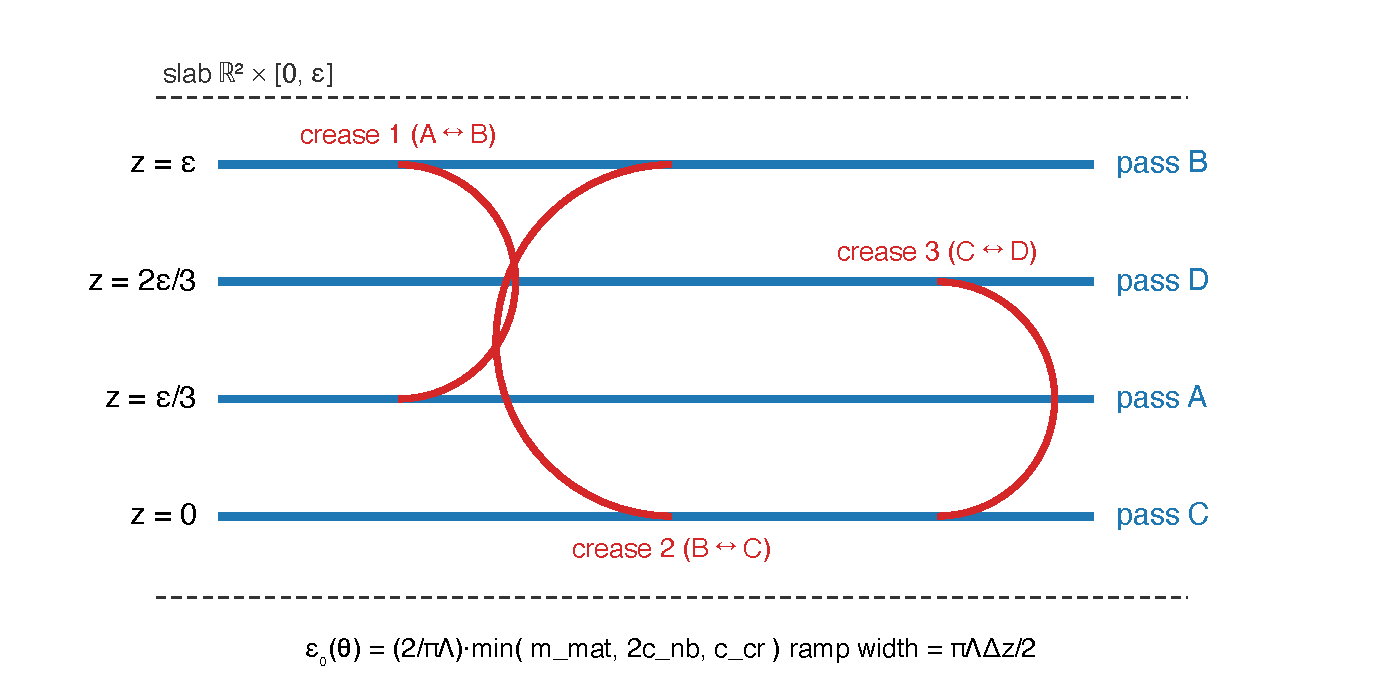
\includegraphics[width=0.9\linewidth]{figs/fig5-slab-ramp.pdf}
\caption{Strong $\varepsilon$-realization of an open state. The four passes are lifted to the constant heights $z_C=0<z_A=\varepsilon/3<z_D=2\varepsilon/3<z_B=\varepsilon$ dictated by the layer order $B>D>A>C$, and each crease is replaced by an isometric hairpin ramp \eqref{eq:hairpin} of radius $r_i$ and collar half-width $\pi r_i/2$. The slab budget $\varepsilon_0(\theta)$ of \eqref{eq:eps0} is exactly what keeps the three collision classes---sheet against sheet, ramp against sheet, ramp against ramp---disjoint.}
\label{fig:slab}
\end{figure}

\subsection{Tight states, necessity, and the equivalence}

Theorem~\ref{thm:openreal} does not apply to zero-clearance states, tight ones in particular: by Observation~\ref{obs:budget} a tight state has $\varepsilon_0=0$, so no room is left for ramps. The remedy is to open the state slightly and then pass to the limit.

\begin{lemma}[Opening]\label{lem:opening}
The pentagonal and dagger states are limits of open valid states with the same layer order. At $\td$ the four-by-four minor of the active-gradient matrix in the $(g,h,a,b)$ columns is exactly nonzero in $\Q[x]/(p_x)$, with value $-0.956\ldots$, so the system $\nabla w_j\cdot\delta=1$ for $j\in\{1,4,5,6\}$ has a solution $\delta$; at the pentagon the explicit rational direction
\begin{equation}\label{eq:openingdir}
  \delta^{\mathrm{op}}=\Bigl(-\tfrac{93}{1000},\ \tfrac{2197}{1000},\ \tfrac{1021}{500},\ \tfrac{509}{250},\ \tfrac{419}{200}\Bigr)
\end{equation}
has all eight wall derivatives rigorously positive, the eight values lying in the interval $[0.984,1.018]$.
\end{lemma}

\begin{proof}
The minor is computed by exact arithmetic in $\Q[x]/(p_x)$ and the interval range for \eqref{eq:openingdir} by interval arithmetic, both in the ancillary suite \cite{anc}. Given such a $\delta$, the walls and the material-consistency functions are rational, hence $C^1$, and the inactive constraints are strict at the tight state, so $w_j(\theta+t\delta)=t\,(\nabla w_j\cdot\delta)+O(t^2)>0$ for every wall and every small $t>0$: the perturbed states are valid and open, and they converge to the tight state as $t\downarrow0$.
\end{proof}

\begin{corollary}[Slack start at the pentagon]\label{cor:slackstart}
For all sufficiently small $t>0$ the state $q_t=P^*+t\,\delta^{\mathrm{op}}$ is slack: every wall satisfies $w_j(q_t)\ge0.98\,t+O(t^2)>0$ by \eqref{eq:openingdir}. The exact directional derivative is
\[
\begin{aligned}
\nabla\core(P^*)\cdot\delta^{\mathrm{op}}
 &=\frac12\left(-\frac{93}{1000}+\frac{2197}{1000}
                  +\frac{1021}{500}+\frac{509}{250}+\frac{419}{200}\right)\\
 &=\frac{8277}{2000}.
\end{aligned}
\]
Since $\core$ is affine on the forward chart,
\[
\core(q_t)=\core(P^*)+\frac{8277}{2000}\,t
\]
holds exactly. The reverse segment $s\mapsto q_{t-s}$, $0\le s\le t$, is therefore a pulling path from the slack state $q_t$ to $P^*$ with strictly decreasing core length. Concatenated with the certified monotone path of Remark~\ref{rem:edge}, this exhibits $\td$ as reachable from slack states, closing the reachability clause of Definition~\ref{def:pull}.
\end{corollary}
\begin{proof}
Positivity of the eight directional derivatives on the stated interval is the interval certificate of Lemma~\ref{lem:opening}; the gradient identity $\nabla\core(P^*)=\tfrac12\mathbf 1$ is Proposition~\ref{prop:gradpent}; the arithmetic is exact. Monotonicity of the concatenation is strict on each segment by the displayed rate and by Remark~\ref{rem:edge}.
\end{proof}

The general statement---that every valid closed state is a limit of open valid states, that is, that the valid set is the closure of its interior in the appropriate semialgebraic sense---is not proved here. Lemma~\ref{lem:opening} establishes exactly the two instances that the main theorems require.

\begin{theorem}[Limit realization of closed states]\label{thm:limitreal}
Let $\bar\theta$ be a valid state satisfying the axioms, with walls allowed to be active, and suppose $\bar\theta=\lim_k\theta_k$ for open valid states $\theta_k$ carrying the same layer order. Then $(f_{\bar\theta},\lambda)$ has a limit realization. In particular $\td$ and the regular pentagon do.
\end{theorem}

\begin{proof}
Take $\varepsilon_k=\frac12\min(\varepsilon_0(\theta_k),1/k)$ and let $F_k$ be the strong realization of Theorem~\ref{thm:openreal} at $\theta_k$. On a compact material set,
\[
  \sup\lvert\pi F_k-f_{\bar\theta}\rvert\le\tfrac\pi4\varepsilon_k+\sup\lvert f_{\theta_k}-f_{\bar\theta}\rvert\longrightarrow0 ,
\]
because $\theta\mapsto f_\theta$ is uniformly continuous on compacta: vertices and directions are rational functions of $\theta$ whose denominators stay bounded away from zero near a valid state. For the separation clause, a compact set $V$ at distance $d_0>0$ from the creases of $\bar\theta$ is at distance at least $d_0/2>C_{\mathrm{ram}}\varepsilon_k$ from the creases of $\theta_k$ for all large $k$, so the constant-height separation \eqref{eq:sheetsep} of $F_k$ applies on $V$, with the same $\lambda$ throughout the sequence. The routine verifications are carried out in the ancillary suite \cite{anc}.
\end{proof}

\begin{lemma}[Mod-2 crossing parity]\label{lem:mod2}
Let $U\subset\R^2$ be an open disc and let $W$ be a compact material region inside a single panel with $f|_W$ a homeomorphism, $\overline U\subset\operatorname{int}f(W)$, and $d(\overline U,\partial f(W))=3\delta_0>0$. Let $F$ be a piecewise $C^2$ embedding with $\sup_W\lvert\pi F-f\rvert<\delta_0$, and put $S=F(W)$. Then every vertical fibre over $U$ meets $S$, and a vertical segment in general position containing the whole $S$-part of its fibre has mod-2 intersection number one with $S$; consequently any piecewise $C^1$ path whose projection stays in $U$, beginning below the entire $S$-part of its fibre and ending above the entire $S$-part of its fibre, must meet $S$. The intersection-theoretic ingredients---transversality, homotopy invariance of the mod-$2$ intersection number for boundaryless targets, and its computation on a fibre---are the standard ones \cite{gp1974}.
\end{lemma}

\begin{proof}
For the first assertion, the straight homotopy $(1-\tau)\pi F|_W+\tau f|_W$ keeps $\partial W$ at distance at least $2\delta_0$ from $\overline U$, so $\deg_2(\pi F|_W,u)=\deg_2(f|_W,u)=1$ for every $u\in U$, and the mod-2 count of a segment covering the whole $S$-part of the fibre equals this degree. For the second, suppose the path $\alpha$ misses $S$, and close it into a cycle $\gamma$ inside the cylinder $\overline U\times\R$: run $\alpha$, rise vertically above the slab, cross horizontally at that height, and descend the initial fibre. The three added pieces contribute $0$, $0$ and, by the first assertion, $1$, so $\gamma\cdot S\equiv1\pmod2$. But $\partial S=F(\partial W)$ projects outside $\overline U$, so $\gamma$ contracts inside the cylinder through the complement of $\partial S$, whence $\gamma\cdot S\equiv\mathrm{lk}_2(\gamma,\partial S)\equiv0$---a contradiction.
\end{proof}

\begin{theorem}[Necessity]\label{thm:necessity}
If a state of the overhand branch has a limit realization, then it satisfies the crease-neighbourhood axiom of Definition~\textup{\ref{def:axiom}}.
\end{theorem}

\begin{proof}
Suppose the axiom fails: a pass $Q$ lying strictly between $P$ and $P'$ in the layer order covers a neighbourhood of an interior point $p_0$ of the crease joining $P$ and $P'$. Choose a short material segment $\sigma$ crossing that crease at $p_0$ whose image remains inside the covered neighbourhood, and perturb it into general position so that the images of its two endpoints avoid all three creases. Let $V_\pm$ be small \emph{fixed} discs about those two endpoint images, at positive distance from the creases and inside the relevant overlap regions. Because the discs are fixed, and not shrinking with $k$, the separation clause of Definition~\ref{def:limitreal} applies on them for all large $k$; it places $F_k(\sigma(-1))$ below and $F_k(\sigma(+1))$ above the entire $S$-part of their respective fibres, where $S=F_k(W)$ for a compact $W\subset Q$ lying over the relevant disc. Lemma~\ref{lem:mod2} then forces $F_k\circ\sigma$ to meet $S$, that is, forces two disjoint material sets to share an image, contradicting injectivity of $F_k$. The point of the argument is that separation is needed only \emph{near the endpoints} of $\sigma$, never at $p_0$ itself, where the crease makes separation impossible; and $\sigma$ may always be taken short enough for its endpoint discs to clear the creases, however small the violated neighbourhood. The routine verifications are carried out in the ancillary suite \cite{anc}.
\end{proof}

\begin{theorem}[Realization completeness for the globally ordered three-crease branch]\label{thm:completeness}
For states $(f_\theta,\lambda)$ of the globally ordered overhand branch $\mathcal B$ (fixing the total layer order $B>D>A>C$), with the opening hypothesis of Lemma~\textup{\ref{lem:opening}} imposed on states of zero clearance, the following are equivalent:
\begin{enumerate}
\item[(a)] the state satisfies the crease-neighbourhood axiom and crease-pair non-crossing (with respect to $B>D>A>C$);
\item[(b)] the state admits a limit realization by embeddings into $\R^2\times[0,\varepsilon_k]$ with $\varepsilon_k\downarrow0$ inducing the order $B>D>A>C$ in the sheet-separation sense.
\end{enumerate}
Here (a) implies (b) unconditionally for open states, and is there strengthened to strong $\varepsilon$-realizations for every $\varepsilon<\varepsilon_0(\theta)$; for states of zero clearance the implication holds under the opening hypothesis, which is certified for $\td$ and for the regular pentagon. The converse implication is unconditional within $\mathcal B$. By contrast, if $\lambda$ is allowed to be an arbitrary pointwise local order, then strong $\varepsilon$-realizability does not force a global total order \textup{(Remark~\ref{rem:cyclic-counterexample})}, though it does wherever all four passes share a common interior point \textup{(Lemma~\ref{lem:common-overlap})}.
\end{theorem}

\begin{proof}
For (a) implies (b): open states are covered by Theorem~\ref{thm:openreal}, and a strong $\varepsilon$-realization for all small $\varepsilon$ yields a limit realization on taking $\varepsilon_k=1/k$; states of zero clearance are covered by Theorem~\ref{thm:limitreal} together with Lemma~\ref{lem:opening}. For (b) implies (a): the crease-neighbourhood axiom is Theorem~\ref{thm:necessity}, and with the global layer order $B>D>A>C$ fixed in $\mathcal B$, the transversality clause of crease-pair non-crossing follows from Proposition~\ref{prop:axred}.
\end{proof}

Theorem~\ref{thm:completeness} is Theorem~\ref{mainthm:realization}.

\begin{remark}[What the axioms actually are]\label{rem:axiomreduction}
Within the globally ordered branch $\mathcal B$, Theorem~\ref{thm:completeness} and Proposition~\ref{prop:axred} separate the independent hypotheses: the crossing datum together with the global total order $B>D>A>C$ (which is forced locally by Lemma~\ref{lem:common-overlap} on the common-overlap locus, but not globally by Remark~\ref{rem:cyclic-counterexample}), and the crease-neighbourhood axiom, from which transverse crease-pair non-crossing follows. That the taco pair $w_9,w_{10}$ appears as a separate pair of walls is a matter of analytic signature rather than logical independence; geometrically, by Observation~\ref{obs:corner}, it is the corner contact of the crease pair $\kappa_1,\kappa_3$.
\end{remark}

\begin{remark}[Numerical remark]\label{rem:slabnumerics}
The clearance values behind Observation~\ref{obs:budget} are $c_{\mathrm{cr}}(\td)=0.0845$ and $m_{\mathrm{mat}}(\td)=1.036$ against $c_{\mathrm{nb}}(\td)=0$, while at the pentagon $c_{\mathrm{nb}}=c_{\mathrm{cr}}=0$ (\texttt{check\_realize}). Along the opening path $\theta_t=\td+t\delta$ of Lemma~\ref{lem:opening} one finds $c_{\mathrm{nb}}(\theta_t)\approx0.96\,t$ and $\varepsilon_0(\theta_t)\approx1.16\,t$, so realizing the state in a slab of fixed height $\varepsilon$ along this path costs an opening $t\gtrsim\varepsilon/1.16$, and then, using $\nabla w_j\cdot\delta=1$ and the multipliers of Theorem~\ref{thm:kkt},
\[
  \core(\theta_t)-\ell^\dagger=\Bigl(\sum_j\lambda_{w_j}\nabla w_j\cdot\delta\Bigr)t+O(t^2)
  =\Bigl(\sum_j\lambda_{w_j}\Bigr)t+O(t^2)\approx4.111\,t ,
\]
in agreement with the measured value $\core-\ell^\dagger=4.11\times10^{-3}$ at $t=10^{-3}$. Composing the two estimates gives $\core(\varepsilon)-\ell^\dagger\lesssim3.5\,\varepsilon$: this construction supplies nearby zero-thickness states in a slab of height $\varepsilon$ with an $O(\varepsilon)$ core-length cost. The coefficient combines the KKT multiplier sum with the chosen opening rate; it is not a material-thickness law or a prediction that physical pulling must stop there. This is an upper bound produced by one particular construction, and no matching lower bound is established, another slab realization possibly doing better. Two further points remain open: whether a state of zero clearance admits a \emph{strong} $\varepsilon$-realization at fixed small $\varepsilon$---the constant-height construction certainly fails there, and a wedge-shaped height assignment is the natural candidate---and the equivalence of the two forms of the induced layer order discussed in Remark~\ref{rem:sheetform}.
\end{remark}

\section{The shape of the tight state, and two predictions}\label{sec:shape}

\subsection{The notched heptagon}
The outline of the folklore state is as simple as an outline can be. At the regular pentagon $P^*$ the boundary of the core has exactly five sides (three creases and two band edges), and every side direction lies in the lattice $36^\circ\mathbb{Z}$; the picture one draws by hand is the picture the model produces (Figure~\ref{fig:pentagon} in Section~\ref{sec:moduli}). At $\td$ the side directions leave that lattice and the outline acquires two further sides. They are small, and they are the whole point: together they cut a notch into one edge.

\begin{proposition}[Shape of $\td$]\label{prop:heptagon}
The core silhouette of $\td$---the boundary of the four passes with $A$ cut at $\ell_2$ and $D$ cut at $y=0$, in the same flush-cut convention as the truncation length---is a mirror-symmetric heptagon $E\,H\,G\,K\,X\,Y\,F$ with exactly one reflex vertex. Here $K=Q_1=I$ is the endpoint of the crease $\kappa_3$ that sits on the far edge $e_B$ of the lay-in band (the active wall $w_5$), while $X=Q_0$ is the other endpoint of $\kappa_3$, and $Y$ is the intersection of $e_B$ with the far edge of the lay-out band. The seven sides measure
\[
|EH|=|GK|=h^\dagger=a^\dagger=1.036386,\qquad |FE|=|KX|=1.050603,
\]
\[
|HG|=1.061053,\qquad |XY|=|YF|=0.051419,
\]
the last two forming a mirror pair of micro-sides carried by the lay-out and the lay-in edge. The interior angles are
\[
\angle E=\angle K=\angle X=\angle F=107.855^\circ,\qquad \angle H=\angle G=109.531^\circ,
\]
together with the reflex angle $\angle Y=249.517^\circ$; they sum to $900^\circ$, as a heptagon requires. The open triangle $XYF$ is covered by none of the four passes: the outline carries a genuine V-notch, cut into one edge and centred on the mirror axis (Figure~\textup{\ref{fig:heptagon}}).
\end{proposition}

\begin{proof}
The seven vertices are rational functions of the coordinates of $\td$. Their squared distances, and the angle cosines after the stated simplifications, admit exact algebraic certificates; the displayed lengths and angles in degrees are rounded evaluations, not claims that angle measures belong to $\Q(x^\dagger)$.

Here is a certificate for the \emph{whole} silhouette. The four flush-cut panels are
\begin{gather*}
A=[E,F,K,G],\quad B=[E,H,G,F],\\
C=[H,G,K,X],\quad D=[X,K,H,E].
\end{gather*}
Exact convex clipping, vertex containment and area identities give
\[
A\cup B=[E,H,G,K,F],\qquad C\cup D=[E,H,G,K,X],
\]
whose intersection is the convex pentagon $I=[E,H,G,K,Y]$.
Their union is $I\cup[E,Y,F]\cup[K,X,Y]$; the three pieces have disjoint interiors. Cancelling their shared edges leaves the simple boundary $EHGKXYF$. Exact orientation tests exclude intersections of nonadjacent boundary edges and show that only $Y$ is reflex. All signs use rational interval evaluation around a Sturm-isolated root of $p_x$; equalities are reduced modulo $p_x$. These are full polygon certificates, not tests at edge midpoints (\texttt{exact\_outline}).

The open triangle $XYF$ also misses the \emph{untruncated} passes. For each pass there is a containing closed half-plane, bounded respectively by $KF$, $GF$, $XH$ and $XE$, whose inward linear functional has signs at $(X,Y,F)$
\[
A:(-,0,0),\quad B:(-,-,0),\quad
C:(0,-,-),\quad D:(0,0,-).
\]
Every point of the open triangle is a strictly positive barycentric combination of its vertices. Each functional is therefore strictly negative there, proving noncoverage by every infinite pass, including both tails.
\end{proof}

\begin{proposition}[The exact notch data]\label{prop:notch}
The squared mouth $|XF|^2$, the squared legs $|XY|^2=|YF|^2$, the squared depth, and the cosine of the reflex angle are elements of $\Q(x^\dagger)$, given by the following polynomials evaluated at $x=x^\dagger$:
\begin{align}
\mathrm{mouth}^2&=-\tfrac{x^{10}}{6}-\tfrac{11x^8}{12}-\tfrac{5x^6}{4}-\tfrac{7x^4}{12}+\tfrac{7x^2}{4}-\tfrac16,\label{eq:notch-mouth}\\
\mathrm{leg}^2&=-\tfrac{x^{10}}{48}-\tfrac{x^8}{6}-\tfrac{5x^6}{24}-\tfrac{x^4}{3}+\tfrac{x^2}{16},\label{eq:notch-leg}\\
\mathrm{depth}^2&=\tfrac{x^{10}}{48}+\tfrac{x^8}{16}+\tfrac{5x^6}{48}-\tfrac{3x^4}{16}-\tfrac{3x^2}{8}+\tfrac1{24},\label{eq:notch-depth}\\
\cos\angle Y&=-\tfrac{x^{10}}{24}-\tfrac{x^8}{8}+\tfrac{x^6}{8}-\tfrac{11x^4}{24}-\tfrac{11x^2}{12}-\tfrac14.\label{eq:notch-angle}
\end{align}
All four polynomials are even, so, exactly as for the multiplier $\lambda_{w_5}$ of Theorem~\textup{\ref{thm:kkt}}, the four displayed quantities lie in the sextic subfield $\Q((x^\dagger)^2)$ rather than in the full degree-twelve field. Numerically, for a strip of width $w$,
\begin{gather*}
\mathrm{mouth}=0.0844877\,w,\qquad \mathrm{leg}=0.0514189\,w,\\
\mathrm{depth}=0.0293149\,w,\qquad \angle Y=249.5170066^\circ.
\end{gather*}
\end{proposition}

\begin{proof}
The seven vertices are rational functions of $\td$, so each squared length is a rational expression in $x^\dagger$; reducing it in the quotient field $\Q[x]/(p_x)$ returns the canonical representatives \eqref{eq:notch-mouth}--\eqref{eq:notch-angle}. Two identities in that quotient are worth recording, since they are what makes the notch a notch. The mirror identity $|XY|^2-|YF|^2$ reduces to exactly $0$, which is also why $\cos\angle Y$ is a field element rather than an expression involving a square root; and the isosceles Pythagorean relation $\mathrm{depth}^2=\mathrm{leg}^2-(\mathrm{mouth}/2)^2$ holds identically, an internal check on four representatives computed independently of one another.
\end{proof}

\begin{figure}[t]
\centering
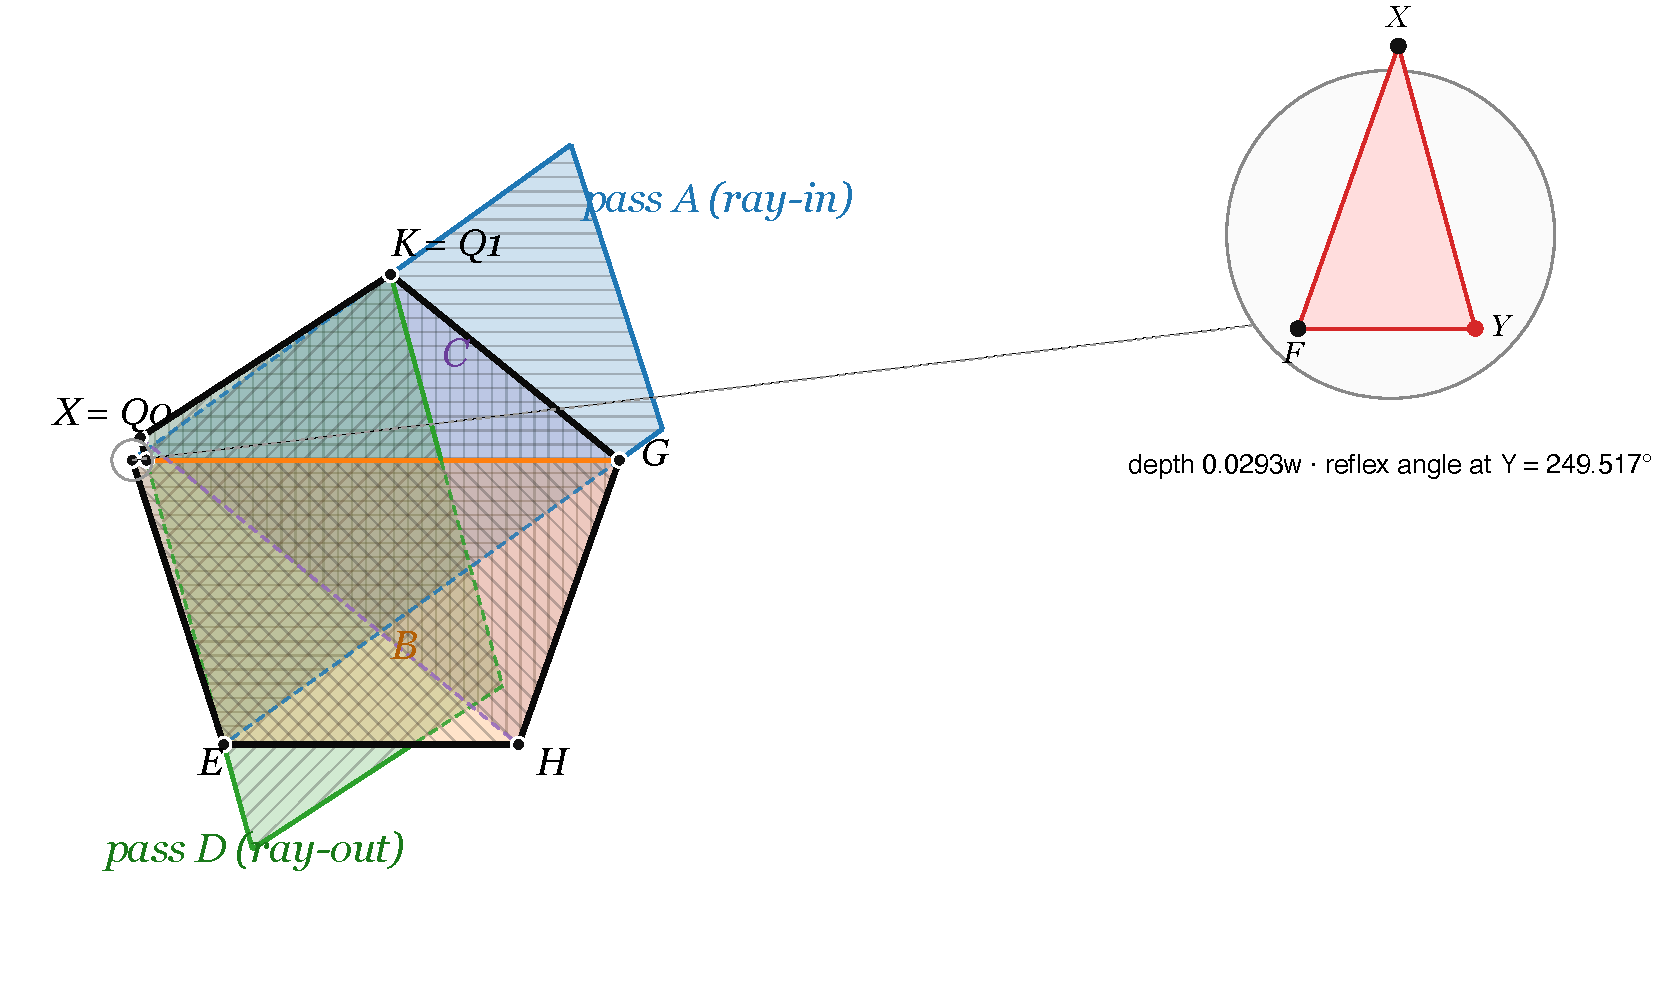
\includegraphics[width=0.95\linewidth]{figs/fig2-heptagon.pdf}
\caption{The tight state $\td$, rendered in the hidden-line convention (solid edges visible, dashed edges passing beneath; creases are the heavy red chords): the mirror-symmetric notched heptagon $E\,H\,G\,K\,X\,Y\,F$, with the V-notch straddling the mirror axis, enlarged in the inset---mouth $0.0845\,w$, legs $0.0514\,w$ for strip width $w$---and quantified exactly in Proposition~\ref{prop:notch}. Compare the five-sided outline of Figure~\ref{fig:pentagon}.}
\label{fig:heptagon}
\end{figure}

\begin{remark}[Contact saturation and symmetry]\label{rem:flushness}
At $P^*$ the eight-wall junction has dihedral symmetry. At the core-length minimum $\td$, Proposition~\ref{prop:heptagon} gives a notched heptagon and Theorem~\ref{thm:s6} gives the associated sextic group $S_6$. Thus tightness alone does not force a regular polygon.
\end{remark}

\begin{remark}[The notch mouth \emph{is} the crease clearance]\label{rem:mouth-clearance}
The mouth $|XF|$ of the notch and the crease clearance $c_{\mathrm{cr}}(\td)=d(\kappa_1,\kappa_3)$ are the same segment. Indeed $X=Q_0$, and the taco parameters at $\td$ satisfy $t=u=1.0506>1$: the intersection of the two crease \emph{lines} lies beyond both crease \emph{segments}, so the minimum distance between $\kappa_1$ and $\kappa_3$ is attained at the endpoint pair $(F,Q_0)$, with both feet at parameter $1$ and the two quantities agreeing to machine precision. This closes a circle with the six-wall identity of the standard slice (Observation~\ref{obs:corner}): on the slice the two creases touch at the shared corner $Q_0=F$, the crease clearance vanishes and the taco pair vanishes identically; moving along the second family opens that contact; and the notch mouth measures precisely how far it has opened by the time tightening stops. In this sense the notch is not a blemish on the tight shape but the geometric record of the descent that produced it.
\end{remark}

\subsection{Two predictions}
In core length the pentagonal and dagger states differ by only $0.114\%$, requiring careful control of material and measurement effects to resolve experimentally. The V-notch provides a second observable. The following predictions refer to the kinematic model.

\begin{remark}[Prediction (i): the notch]\label{rem:pred-notch}
\emph{Within the kinematic model}, the certified pulling path terminates not at the pentagon but at the notched heptagon $\td$ of Theorem~\ref{thm:sosc}, with the four exact quantities of Proposition~\ref{prop:notch}: mouth $0.0845w$, legs $0.0514w$, depth $0.0293w$, and reflex angle $249.52^\circ$. On a $2\,\mathrm{cm}$ tape this is a notch about $1.7\,\mathrm{mm}$ wide and $0.6\,\mathrm{mm}$ deep, visible to the eye and straightforward to measure. Real paper may instead lock at the pentagon: friction at eight simultaneous contacts, creases pinned by the material rather than free to move, or a thickness cost exceeding the $0.114\%$ core gain would each arrest the descent at the pass. Measuring the notch distinguishes the predicted outlines of the two optima.
\end{remark}

\begin{remark}[Prediction (ii): a slab-construction cost]\label{rem:pred-thickness}
Along one certified opening direction, our constant-height hairpin construction realizes nearby open states at cost
\[
\Delta\ell\;\approx\;\Bigl(\sum_j\lambda_{w_j}\Bigr)t(\varepsilon)\;\lesssim\;3.5\,\varepsilon .
\]
The reasoning is a first-order trade between two linear rates along the opening direction $\delta$ of Lemma~\ref{lem:opening}. On one side, the KKT identity of Theorem~\ref{thm:kkt} turns the cost of opening into the sum of the multipliers,
\[
\core(\theta_t)-\ell^\dagger=(\nabla\core\cdot\delta)\,t+O(t^2)=\Bigl(\sum_j\lambda_{w_j}\Bigr)t+O(t^2)\approx4.11\,t;
\]
on the other, the realizable slab budget grows linearly from zero along the same path, $\varepsilon_0(\theta_t)\approx1.16\,t$, so a state realized by \emph{this construction} in a slab of height $\varepsilon$ sits at $t\gtrsim\varepsilon/1.16$ along the path. Combining the two rates gives the stated law. Its interpretation is the content of the prediction: \emph{the KKT multipliers are the unit prices of the ramp clearances}. Each active wall is a clearance that tightening has spent, and $\lambda_j$ is the core length bought per unit of clearance handed back, which is why the coefficient is a sum of multipliers and not a geometric constant. Two caveats. This is an $O(\varepsilon)$ \emph{upper} bound produced by one particular opening path; the matching lower bound is not established, and a different slab realization might do better than anything on that path. And the coefficient $3.5$ inherits the numerical status of $\varepsilon_0$, whereas $\sum_j\lambda_{w_j}$ is exact.
\end{remark}

\begin{remark}[Static realization is not dynamic tightening]\label{rem:static-dynamic}
Theorem~\ref{mainthm:realization} lifts \emph{individual} states into slabs, one $\varepsilon$ at a time. Lifting an entire tightening path into a \emph{single} slab of fixed height is a different statement, and it is not proved here; it is posed as open problem~\ref{op:lifting} below. Both predictions should be read with that gap in view.
\end{remark}

\section{Toward global uniqueness: a stratified census}\label{sec:census}

Everything established so far is local. Theorem~\ref{thm:sosc} makes $\td$ a strict local minimizer of $\core$ and Theorem~\ref{thm:pass} makes the pentagon a pass, but neither excludes a further blocked state elsewhere in $\M$. This section closes that gap as far as we can, in two stages: first a descent census, which is evidence, and then a stratified census of first-order blocked points, which is a classification carrying per-candidate certificates.

\begin{remark}[Descent census]\label{rem:descent-census}
Three independent multistart sweeps (different seeds, perturbations of size $\pm0.03$ to $\pm0.20$ around slice states with $x\in[0.10,0.32]$) produced $286$ valid starting points, and all $286$ converged to the single attractor $\td$, with terminal spread at most $1.2\times10^{-7}$ and $|\ell-\ell^\dagger|\le2.3\times10^{-13}$. Every terminal active set was exactly $\{w_1,w_4,w_5,w_6\}$. No local minimum other than $\td$ was found, and no run stalled at the pentagon corner: random descent passes straight through the pass, a dynamical reproduction of Theorem~\ref{thm:pass}.
\end{remark}

The coverage of Remark~\ref{rem:descent-census} has three limits. The region $x<0.10$ was not sampled; strata on which a taco wall is active cannot be reached by this method, since they lie far from the sampled region; and starts placed on the boundary strata themselves were not tested. An independent verification pass reproduced a sample of the descents and extended the coverage with distant probes (valid starting points at max-norm distance $4.7$ from the slice), which again reached $\td$. This is strong numerical evidence for global uniqueness; it is not a proof, and the route to one is symbolic elimination over the remaining strata (open problem~\ref{op:uniqueness}).

The classification replaces descent by first-order blocking. Recall that a valid state is \emph{blocked} when $\nabla\core$ lies in the cone generated by the gradients of the walls active at it, taken within the relevant branch of the disjunctive taco pair: the first-order statement that no feasible direction decreases the core length. Blockedness is what tightening produces, and it is independent of how, or whether, a state is reached. Its relation to the active-set geometry is governed by the constraint qualification in force, and here the taco pair rules out the stronger of the two standard ones.

Recall Observation~\ref{obs:corner}: $w_9=w_{10}=0$ exactly when $Q_0=F$, a three-dimensional locus $\mathcal F$ on which the four active wall gradients have rank two, so LICQ fails identically. The locus meets the valid region, and the standard symmetric slice is exactly $\mathcal F\cap\{w_1=w_4=0\}$. Numerically, the valid locus on which six or more walls are active consists of the slice and the pentagon alone.

Because LICQ fails on $\mathcal F$, the census is formulated under the weaker Mangasarian--Fromovitz condition (MFCQ): the existence of a direction strictly increasing every wall active on the relevant taco branch \cite{nocedal2006}.

\begin{theorem}[Stratified census; $=$ Theorem~\textup{\ref{mainthm:census}}]\label{thm:census}
Let $\theta$ be a tight state at which MFCQ holds for the relevant taco branch. Then $\theta$ is blocked; and by the cone form of Carath\'eodory's theorem every blocked point solves the square KKT system of an active set $S$ with $|S|\le5$ containing at most one taco wall. The enumeration runs over all active sets of size at most five, both-taco sets included as redundant super-captures, less the four subsets of $\{w_4,w_6\}$ excluded by the $x$-independence lemma: $215$ strata, capturing all candidates, including those sitting at high-activity corners. Across all $215$ strata the only \emph{certified} surviving blocked state is $\td$; the residual components are computational and are itemized in the proof and in Table~\ref{tab:census}. The pentagon occurs as a root of the KKT system in twenty of them and is excluded in each by the single exact Farkas certificate of Theorem~\textup{\ref{thm:pass}} together with cone monotonicity.
\end{theorem}

\begin{proof}[Proof of Theorem~\textup{\ref{thm:census}}]
\emph{Tight and MFCQ imply blocked.} Suppose a tight state $\theta$ is not blocked on its taco branch. By the Farkas alternative there is a direction $d$ with $\nabla\core\cdot d<0$ and $\nabla w_i\cdot d\ge0$ for every active wall $i$; MFCQ supplies $e$ with $\nabla w_i\cdot e>0$ for all active $i$, and $\tilde d=d+\eta e$ with $\eta>0$ small satisfies $\nabla\core\cdot\tilde d<0$ and $\nabla w_i\cdot\tilde d>0$ simultaneously. For small $t>0$ the segment $\theta+t\tilde d$ then keeps every active wall strictly positive by first-order Taylor expansion, keeps the inactive walls and the (open) branch conditions by continuity, and strictly decreases $\core$: a pulling path issuing from $\theta$ that decreases the core length, contradicting tightness. On the taco union the argument is applied on each branch separately.
The grades inside the statement are not uniform, and the split is worth spelling out. The \emph{reduction} is proved. MFCQ is certified exactly at $P^*$ and at $\td$: rank-$4$ LICQ at $\td$, by a $4\times4$ minor of the active-gradient matrix that is nonzero in $\Q[x]/(p_x)$, and at the pentagon an explicit rational direction whose eight wall derivatives are rigorously positive under interval evaluation. The Carath\'eodory step is a theorem about cones \cite{barvinok2002}, and it is what licenses the truncation to $|S|\le5$ and to at most one taco wall: strata with both taco walls active are redundant super-captures of strata already on the list, so no candidate escapes through them. The \emph{arithmetic} is exact as well. All eight wall functions admit $\mathbb{Z}$-coefficient polynomial representatives, of degrees $(2,16,4,16,4,16,5,3)$ in the order $(w_1,w_4,w_5,w_6,w_7,w_8,w_9,w_{10})$, and $\core=(x+g+h+a+b)/2$ is affine. Clearing the wall denominators on their nonzero sign domains therefore gives a polynomial KKT system for each stratum. Polynomialization multiplies each wall by a scale factor whose sign is itself part of the bookkeeping: it is positive unconditionally for $w_1,w_4,w_6,w_7,w_8$, and only on the relevant branch for $w_5,w_9,w_{10}$. In the variable $q=g-h$, the final encoding uses $c_5=(q+x)(1-qx)$ but $c_7=(q^2+1)(x^2+1)>0$; the latter requires no extra sign condition. The certificates accordingly either use the unconditional walls alone or co-certify the scale. The census is run over the computational chamber $\Mhat$; its stratum systems are domain-free polynomial systems and no recorded disposition invokes the taco sign, so the dispositions read verbatim over the honest moduli; within the computational harvest, the extra honest region $\{t\le0\}\cup\{u\le0\}$ produced no harvested candidate---per-stratum completeness of the harvest remaining, as elsewhere, a numerical component.

Two exact exclusions simplify the census. The second excludes particular roots, not whole strata. Those with $S\subseteq\{w_4,w_6\}$ carry no blocked point at all, because $w_4$ and $w_6$ are independent of $x$ while $\partial\core/\partial x\equiv\frac12$ globally; and every occurrence of the pentagon as a KKT root is excluded by the Farkas certificate of Theorem~\ref{thm:pass}. On the stratum $\{w_1,w_4,w_5,w_6\}$ the unique KKT point is $\td$ itself, by the reduction to the plane curve $N_5$ and the minimal polynomial $p_x$. That leaves $104$ harvested candidates elsewhere. Of these, all $72$ that admit a certifiable regular root carry per-candidate Krawczyk root enclosures together with interval-sign exclusions on those root-isolating boxes---using unconditionally scaled walls, scale-co-certified conditional walls, or direct interval evaluation of a true wall (in fact, \texttt{exact\_census\_roots} freshly isolates all $72$ roots in $100$-digit \textsc{Arb} ball arithmetic and certifies that every one violates a true geometric sliver wall strictly below $-0.315$ on its isolated root box)---and those exclusions are rigorous.

\begin{compres}[The numerical residue, localized]\label{compres:residue}
For the remaining $32$ candidates the Krawczyk operator is inconclusive, so whether a genuine stratum root exists near them remains open. Classifying their saved approximate centres gives four with $x<0$, six with $|q+x|<10^{-6}$, eighteen with $|1-qx|<10^{-6}$ (the second factor of the $w_5$-denominator $c_5=(q+x)(1-qx)$), and four remaining centres (all with $h,a<0$); none satisfies $q+x=0$ or $1-qx=0$ exactly as stored decimals. At radius $10^{-12}$ around every one of the $104$ saved centres, a true sliver wall is certified below $-0.315$ in both \textsc{Arb} and \texttt{mpmath} interval arithmetic (the reported maximum active-wall residual of $19.5$ occurring at a floating-point denominator of order $2.1\times10^{-15}$). Beyond this, the numerical residue of Theorem~\ref{thm:census} is confined to three isolated components: the per-stratum completeness of the harvest, that is, that no real root of a stratum's KKT system was missed by multistart; the absence of valid states at which MFCQ fails, verified numerically on $\mathcal F$; and the calibration of the on-branch multiplier scales. Each has a concrete symbolic route, described in open problem~\ref{op:uniqueness}. The completeness component is doubly implemented: two independent constructions of the wall system, rational expression trees with $30$ seeds per stratum and polynomialized walls with $100$, return identical outcomes, with $\td$ the only candidate passing every filter in both. For reference, the chart-coordinate wall representatives are compact: with $q=g-h$, the wall $w_1$ has integer representative $2gx+x^2-1$ over denominator $1$; the walls $w_4,w_6,w_8$ share the manifestly positive denominator $(q+a-b)^2+1$ and $w_7$ the denominator $q^2+1$, with quartic numerators; $w_5$ has the branch-signed denominator $(q+x)(qx-1)$, the census scale factor $c_5$ up to sign; and the taco pair shares one cubic denominator, the line-pair determinant of $\kappa_1,\kappa_3$, with $w_{10}$'s numerator equal to $b\,(q^2+2qx-1)+h\,(q^2+1)$. The degrees quoted above are those of the \emph{eliminated} polynomializations used by the census, not of these chart representatives; both encodings, in machine-readable form, are \texttt{uniq\_setup} and \texttt{uniq\_poly} in the suite. The sixty-seven archived sliver-sign exclusions (and seventy-one wall exclusions in a fresh run) are additionally re-verified in the ball arithmetic of \textsc{Arb} (\texttt{arb\_recheck}), independently of \texttt{mpmath}. Table~\ref{tab:census} collects the split.
\end{compres}
\end{proof}

\begin{table}[t]
\centering\small
\begin{tabular}{@{}p{0.56\linewidth}l@{}}
\hline
Ingredient of Theorem~\ref{thm:census} & Status\\
\hline
\raggedright Tight and MFCQ imply blocked; MFCQ certificates at $P^*$ and $\td$ & exact\tabularnewline
\raggedright Carath\'eodory reduction to $|S|\le5$ with at most one taco wall & proof\tabularnewline
\raggedright Wall polynomialization, rationality of $\core$, the manifold $\mathcal F$ & exact\tabularnewline
\raggedright Emptiness of the strata $S\subseteq\{w_4,w_6\}$; exclusion of all pentagon root copies & exact\tabularnewline
\raggedright Uniqueness of $\td$ on the stratum $\{w_1,w_4,w_5,w_6\}$ & exact\tabularnewline
\raggedright Exclusion of the $72$ candidates with certifiable regular roots & interval\tabularnewline
\raggedright Exclusion of the $32$ candidates with inconclusive Krawczyk operator & numerical\tabularnewline
\raggedright Per-stratum completeness of the harvest; absence of valid non-MFCQ points; on-branch scale calibration & numerical\tabularnewline
\hline
\end{tabular}
\caption{Verification grades inside the stratified census. Here \emph{exact} means symbolic computation in $\Q$, $\Q(\sqrt5)$, or $\Q[x]/(p_x)$; \emph{interval} means a machine-checked enclosure argument; and \emph{numerical} means floating-point evidence with the residue localized as stated.}
\label{tab:census}
\end{table}

Two closing remarks on what the census does and does not say. It classifies \emph{blocked} points, so it is insensitive to reachability: descent along the certified path of Theorem~\ref{mainthm:pass} reaches $\td$, while the behaviour of generic descent remains the numerical statement of Remark~\ref{rem:descent-census}. And it is a classification of first-order behaviour only; the strictness of the minimum at $\td$ comes from the exact reduced Hessian of Theorem~\ref{thm:sosc}, not from anything in this section.

\section{Beyond the trefoil: an exact blocked hexagon for the figure-eight knot}\label{sec:figure8}

Everything so far concerns the unique three-crease branch. This section runs the same program---enumerate, build the moduli space, tighten, identify, certify---one crossing higher, and proves Theorem~\ref{mainthm:hex}. The outcome is a second data point for the general theory, and a striking one: where the trefoil produced a degree-twelve certified minimizer outside the reach of radicals, the figure-eight produces a certified blocked minimizer in a quadratic field.

\subsection{The branch}
Running the enumeration machinery of Theorem~\ref{mainthm:fold} at four creases (block-ordered cyclic codes, Gauss parity, planarity of the rotation systems) yields exactly one irreducible four-crossing code, $\mathtt{XYZXWZYW}$ in the crossing alphabet of Section~\ref{sec:model}, with exactly two planar rotation systems forming a mirror pair. Evaluating the Kauffman bracket over all sixteen over/under assignments shows that exactly two produce the Jones polynomial of the figure-eight knot $4_1$ (a mirror pair, as amphichirality requires), two that of the trefoil, and twelve that of the unknot. The naming does not rest on the Jones polynomial, which is not a complete invariant. The shadow code of the branch and the shadow code of the standard figure-eight diagram canonicalize to the same cyclic word; the shadow admits exactly two planar rotation systems, a mirror pair; and the two surviving assignments are precisely the two alternating decorations of that shadow. Hence the two decorated diagrams \emph{are} the standard figure-eight diagram and its mirror, up to homeomorphism of the plane, and the knot is $4_1$ by definition; the bracket computation is the search that isolated them. The figure-eight is therefore the unique new knot arising from the irreducible four-crossing code---codes with five or six crossings, permitted at $n=4$ by the crossing bound, are enumerated combinatorially but their knots are not classified here---and it determines a branch $\mathcal B_{4_1}$ whose centreline chart $(\tau_1,\ldots,\tau_4,L_1,L_2,L_3)$ has dimension $2n-1=7$, in agreement with the dimension count of Proposition~\ref{prop:dim}.

A long diagram cuts the closed code at a base point and distributes the eight crossing visits among five straight passes $P_0,\ldots,P_4$; a \emph{cell} of the branch records which pass pairs cross and under which layer order (Figure~\ref{fig:f8code}). Two constraints prune the combinatorics before any geometry is computed: a straight pass can cross only non-adjacent passes, and the over/under pattern of a $4_1$ assignment must extend to a total layer order, that is, the pairwise above/below relations it forces must be acyclic. A rerun of $8\times10^6$ sampled configurations with the actual crease-capped panel oracle found the candidate cell: \emph{the figure-eight knot does fold flat at width one with four creases}, and every valid state found---$21$ distinct states, each recorded twice, once for each top--bottom flip---lies in a single cell, with crossing pairs $\{(0,2),(0,3),(1,4),(2,4)\}$, self-mirror under material reversal, and layer order $P_1>P_4>P_2>P_0>P_3$ up to the flip; the two flip records per state are an accounting identity, not an observation. The rerun uses eight independent random streams with seeds $7000,\ldots,7007$, each generating $10^6$ configurations with the turn magnitudes sampled uniformly from $[0.3,3.1]$ and the three lengths from $[0.3,4.0]$. Half the sign-pattern draws choose a common turn sign, and half choose four independent signs. The oracle tests the actual oblique crease caps, unbounded tails, the layer axiom, and centreline general position; its source snapshots, tolerances, seeds and all accepted states are recorded by \texttt{n4\_rerun}. The turn sign pattern is $(+,+,-,-)$: where the tightened trefoil winds as a spiral, the figure-eight folds as a point-symmetric zigzag, the geometric expression of its amphichirality. Existence has since been upgraded to exact---the state $\theta^*_{4_1}$ of Theorem~\ref{mainthm:hex} is itself certified valid, all six forbidden crease/pass intersections tested against the actual convex panels by exact affine half-plane clipping in $\Q(\sqrt{15})$ (\texttt{n4\_exact\_valid})---while the exhaustiveness of the cell remains a numerical statement, graded as such (Figure~\ref{fig:f8loose}).

\begin{figure}[t]
\centering
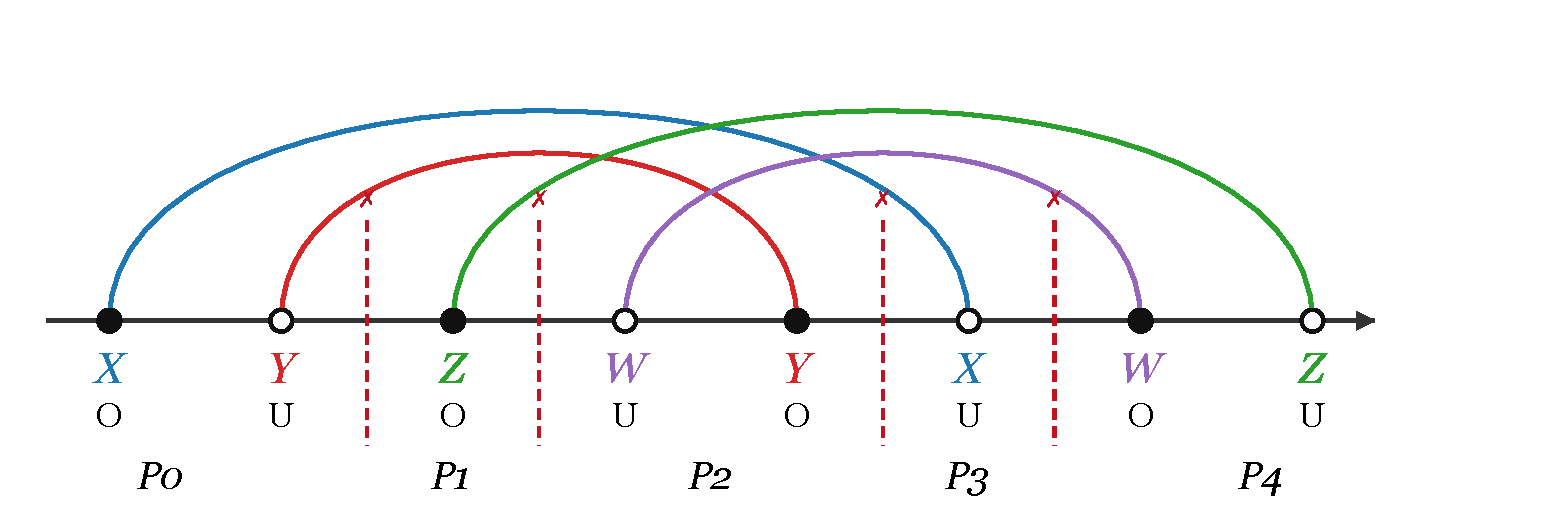
\includegraphics[width=0.9\linewidth]{figs/fig41-code.pdf}
\caption{The realized cell as combinatorics. The material line carries one rotation of the canonical code, with the crossings relabelled, read $X\,Y\,Z\,W\,Y\,X\,W\,Z$, with the alternating over/under pattern of the $4_1$ assignment (filled = over); the four cuts (dashed) distribute the eight visits into the passes $P_0,\dots,P_4$, producing the crossing pairs $X\colon(0,3)$, $Y\colon(0,2)$, $Z\colon(1,4)$, $W\colon(2,4)$ of the cell, with layer order $P_1>P_4>P_2>P_0>P_3$.}
\label{fig:f8code}
\end{figure}

\begin{figure}[t]
\centering
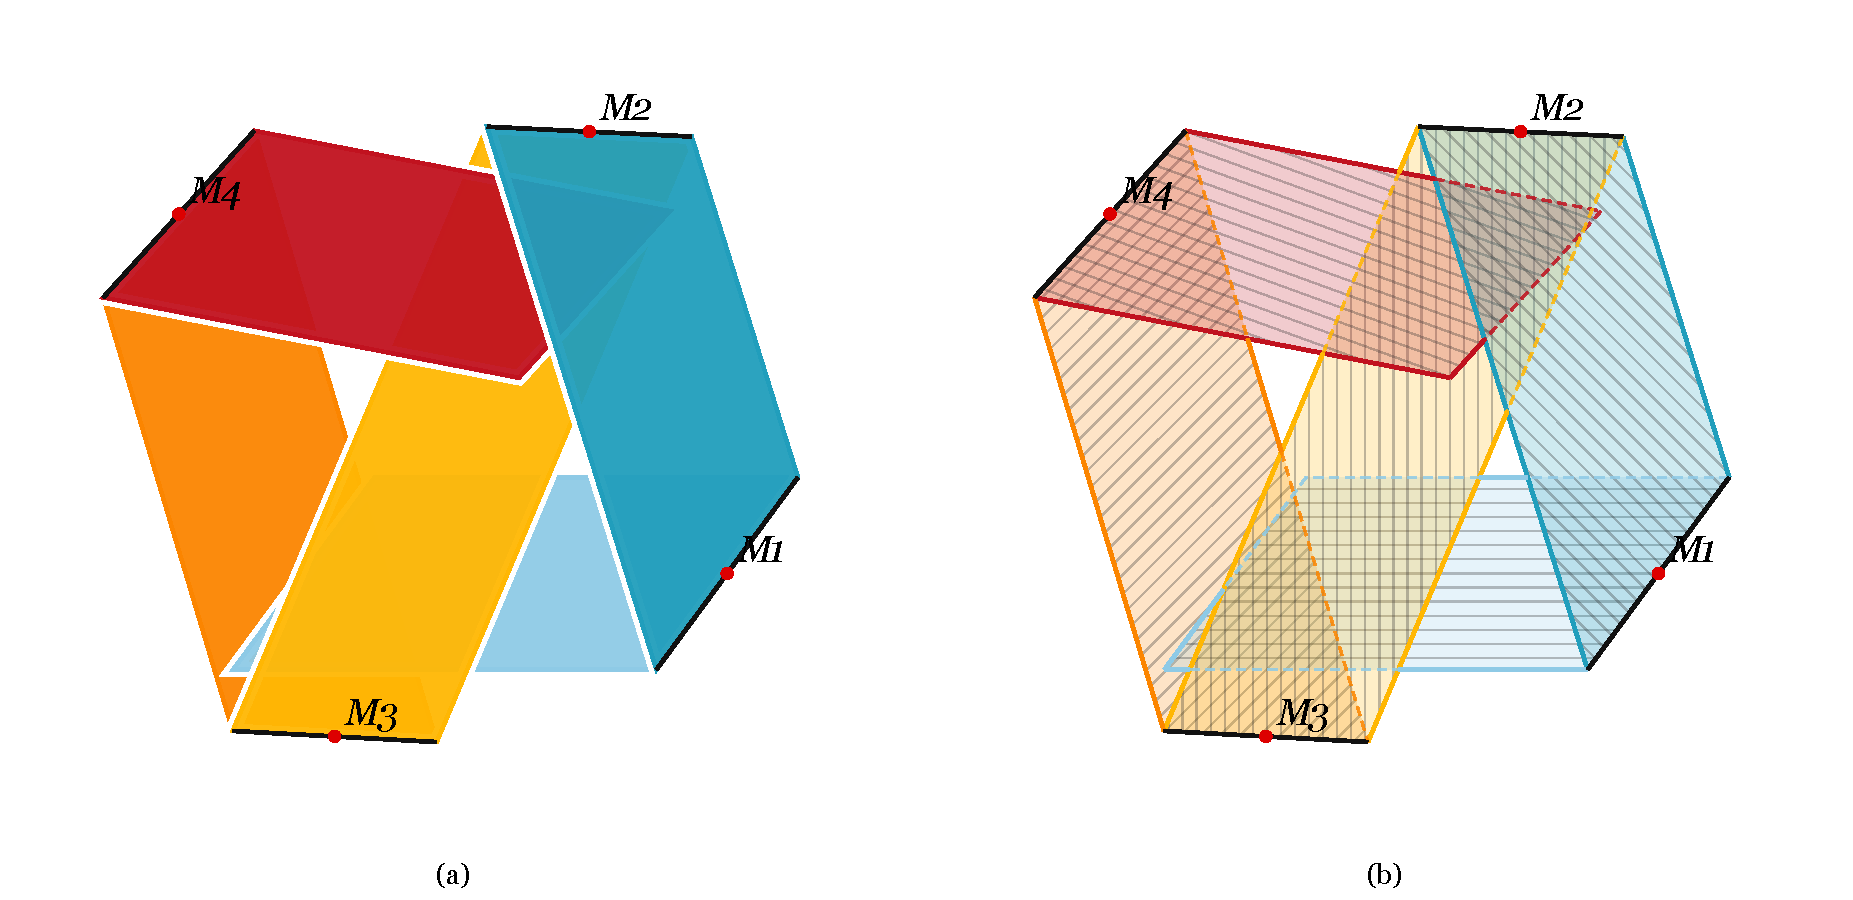
\includegraphics[width=\linewidth]{figs/fig41-loose.pdf}
\caption{A valid width-one flat folded figure-eight state before tightening ($\core\approx8.65$): (a) the state as seen from above; (b) its structure, dashed edges passing beneath. Fold points $M_1,\ldots,M_4$ are marked; crease chords are the heavy segments; the two rays are the tails. The weave is the point-symmetric zigzag cell described in the text.}
\label{fig:f8loose}
\end{figure}

The crossing shadow alone can admit an unknot layering at $\core\approx2.66$. Among its sixteen assignments the integer determinants are $1$ (twelve times), $3$ (twice) and $5$ (twice). A Fox five-colouring count of $25$ selects precisely the figure-eight pair. For the crease-neighbourhood condition, the half-planes of each actual pass pull back to affine inequalities along a crease. Intersecting the resulting parameter intervals tests its full relative interior. A grid of $31$ points can miss a penetration of depth $0.031$ in the final three percent of a chord, admitting an apparent minimum $0.096$ below the certified contact-chamber candidate. The search uses the interval-intersection rule with explicit floating-point tolerances. The point and opening certificates use ordered algebraic fields.

\subsection{The tight state, exactly}
Fixing the layer order, the corrected-oracle rerun descends $\core=L_1+L_2+L_3$ from all $42$ state--layering records. With the recorded finite search budget, $31$ endpoints have core length within $0.01$ of $4\sqrt{15}/3$; this threshold measures proximity in objective value, not certified convergence in configuration space. At each of the other $11$ endpoints, a linear-programming direction followed by $101$ actual-panel checks along a short ray gives a numerically feasible decrease. These sampled rays are evidence of optimization stalls, not interval-certified continuous paths or a complete Farkas classification. The exact state identified from this search is symmetric under material reversal, $\tau_4=-\tau_1$, $\tau_3=-\tau_2$, $L_3=L_1$, and its active set consists of eight contacts of exactly the kind the trefoil walls led us to expect: the endpoints of crease chords $1$ and $4$ against the bands of the passes between them in the layer order, and---the new feature---crease chords $2$ and $3$ lying \emph{parallel along} a band edge, a corner contact in which both chord endpoints touch simultaneously. On the symmetric slice these eight conditions reduce to four equations in $(\tau_1,\tau_2,L_1,L_2)$, a zero-dimensional square system. Newton at $60$ digits, integer-relation identification, and symbolic verification then give the exact solution of Theorem~\ref{mainthm:hex}:
\begin{gather*}
\cos\tau_1^*=-\tfrac14,\qquad \tau_2^*=2\pi-2\tau_1^*,\qquad
L^*=\tfrac{1}{\sqrt{15}}\,(6,\,8,\,6),\\
\core(\theta^*_{4_1})=\tfrac{20}{\sqrt{15}}=\tfrac{4\sqrt{15}}{3}=5.16397\ldots
\end{gather*}
Every contact equation, and the coincidences behind them, are verified exactly in $\Q(\sqrt{15},\sqrt{10},\sqrt6)$: the two tails are antiparallel, with offset exactly the strip width ($M_4=({-}\tfrac{\sqrt{15}}3,1)$ with the incoming centreline on $y=0$); the second crease chord lies on the line $y=\tfrac32$ carrying the upper edge of the outgoing band, and by material reversal the third on $y=-\tfrac12$; and the crease chords meet pairwise at two double points,
\[
E_2^+=E_4^+=\big({-}\tfrac{7\sqrt{15}}{30},\tfrac32\big),\qquad
E_1^-=E_3^-=\big({-}\tfrac{\sqrt{15}}{10},-\tfrac12\big),
\]
so the four creases close into a chain---the figure-eight analogue of the corner contact $Q_0=F$ of Observation~\ref{obs:corner}. For clarity, the smooth contact chamber used for optimality is defined explicitly. Set $d_j=(\cos\phi_j,\sin\phi_j)$ with $\phi_j=\sum_{i=1}^j\tau_i$, $\phi_0=0$, and
\[
V_i^\pm=M_i\pm\frac{d_{i-1}+d_i}{2\sin\tau_i}.
\]
These labels use the signed chord-vector convention, independently of the geometric $E_i^\pm$ labels above. Define $f_j(P)=\operatorname{cross}(d_j,P-O_j)$, where $O_0=M_1$, $O_2=M_2$, and $O_4=M_4$. The eight functions are
\begin{align*}
g_1&=-f_4(V_1^+)-\tfrac12,& g_2&=f_2(V_1^-)-\tfrac12,\\
g_{3a}&=f_4(V_2^+)-\tfrac12,&g_{3b}&=f_4(V_2^-)-\tfrac12,\\
g_1'&=f_0(V_4^+)-\tfrac12,&g_2'&=-f_2(V_4^-)-\tfrac12,\\
g_{3a}'&=-f_0(V_3^+)-\tfrac12,&g_{3b}'&=-f_0(V_3^-)-\tfrac12.
\end{align*}
Let $\mathcal C$ be the set on which all eight are nonnegative, restricted to the nondegenerate coordinate neighbourhood under discussion. The KKT certificate is exact: for these constraints, the stationarity system $\nabla\core=\sum\lambda_i\nabla g_i$ has an exact solution with all multipliers positive in $\Q(\sqrt{15})$,
\[
\lambda=\tfrac{\sqrt{15}}{45}\,\big(21,\;3,\;21,\;13,\;4,\;17,\;5\big)
\]
on the ordered subset $(g_1,g_{3a},g_{3b},g_1',g_2',g_{3a}',g_{3b}')$, with residual identically zero; its gradient determinant is $-\sqrt{15}/2$. This is an exact blocked certificate for the smooth contact chamber $\mathcal C$ used by the optimizer, and was obtained by the same identify-then-verify route; the Jacobian lives in $\Q(\sqrt{15})$ because the chord vector of a crease simplifies to $(d_i+d_{i+1})/(2\sin\tau_{i+1})$, eliminating all half angles. Two upgrades come free. The active gradients have rank seven with all multipliers positive on an invertible seven-generator subsystem, so every nonzero direction of the linearized cone strictly increases $\core$: blocking is \emph{strict local minimality on $\mathcal C$}, by the same first-order sufficiency mechanism as at the pentagon. To extend this statement to the entire geometric cell one must prove that every nearby valid configuration satisfies these eight inequalities. In particular, simultaneous endpoint/cap contacts can have alternate local branches; a sampled wall inventory does not establish their necessity. We therefore retain the contact-chamber qualification. And, exactly, the state is no isolated boundary artefact: the direction $v$ that fixes all four angles and scales the lengths in the ratio $(2,3,2)$ satisfies $\nabla g_k\cdot v=1$ for \emph{all eight} contacts, as an identity in $\Q(\sqrt{15})$, so every contact opens at unit rate along $v$; \texttt{n4\_exact\_opening} verifies actual panel non-penetration on the entire interval $0<s\le10^{-3}$ along this direction, using exact affine half-plane inequalities, so $\theta^*_{4_1}$ is a limit of open valid states. That limit statement upgrades to reachability:

\begin{lemma}[Slack start and reachability at the hexagon]\label{lem:slackstart41}
For all sufficiently small $s>0$ the state $q_s=\theta^*_{4_1}+s\,v$ is a slack state of the figure-eight branch: each active contact satisfies $g_k(q_s)=s+O(s^2)>0$ by the exact unit rates, the actual panels are separated from every forbidden crease by the exact half-plane certificate, and the open diagram conditions persist by continuity. Moreover,
\[\core(q_s)=\tfrac{4\sqrt{15}}3+\tfrac{28\sqrt{15}}{15}\,s,\qquad \nabla\core\cdot v=\tfrac{28\sqrt{15}}{15}=\textstyle\sum_j\lambda_j\ \text{exactly}.\]
The reverse path $s\mapsto q_{s_0-s}$ is a branch-preserving pulling path with strictly decreasing core length terminating at $\theta^*_{4_1}$; combined with the blocked certificate, $\theta^*_{4_1}$ is reachable from slack states and \emph{tight within $\mathcal C$} in the sense of Definition~\ref{def:pull}. Tightness against paths leaving this contact chamber is not asserted.
\end{lemma}

\begin{proof}
The contact functions along the fixed-angle opening path are affine in $s$. The exact unit derivatives make them positive. More decisively, \texttt{n4\_exact\_opening} checks the actual obliquely capped panels: each forbidden crease is separated by a pass half-plane throughout $0<s\le10^{-3}$. Thus this is a continuous-interval certificate, not a finite list of tested radii. The diagram remains in the same cell for sufficiently small $s$ by its strict crossing margins. The identity $\nabla\core\cdot v=\sum_j\lambda_j$ follows from the exact KKT representation and unit contact rates. Reversing the path decreases the affine core length and reaches the state; the contact-chamber strict minimum excludes further decreasing paths within $\mathcal C$.
\end{proof}

\begin{figure}[t]
\centering
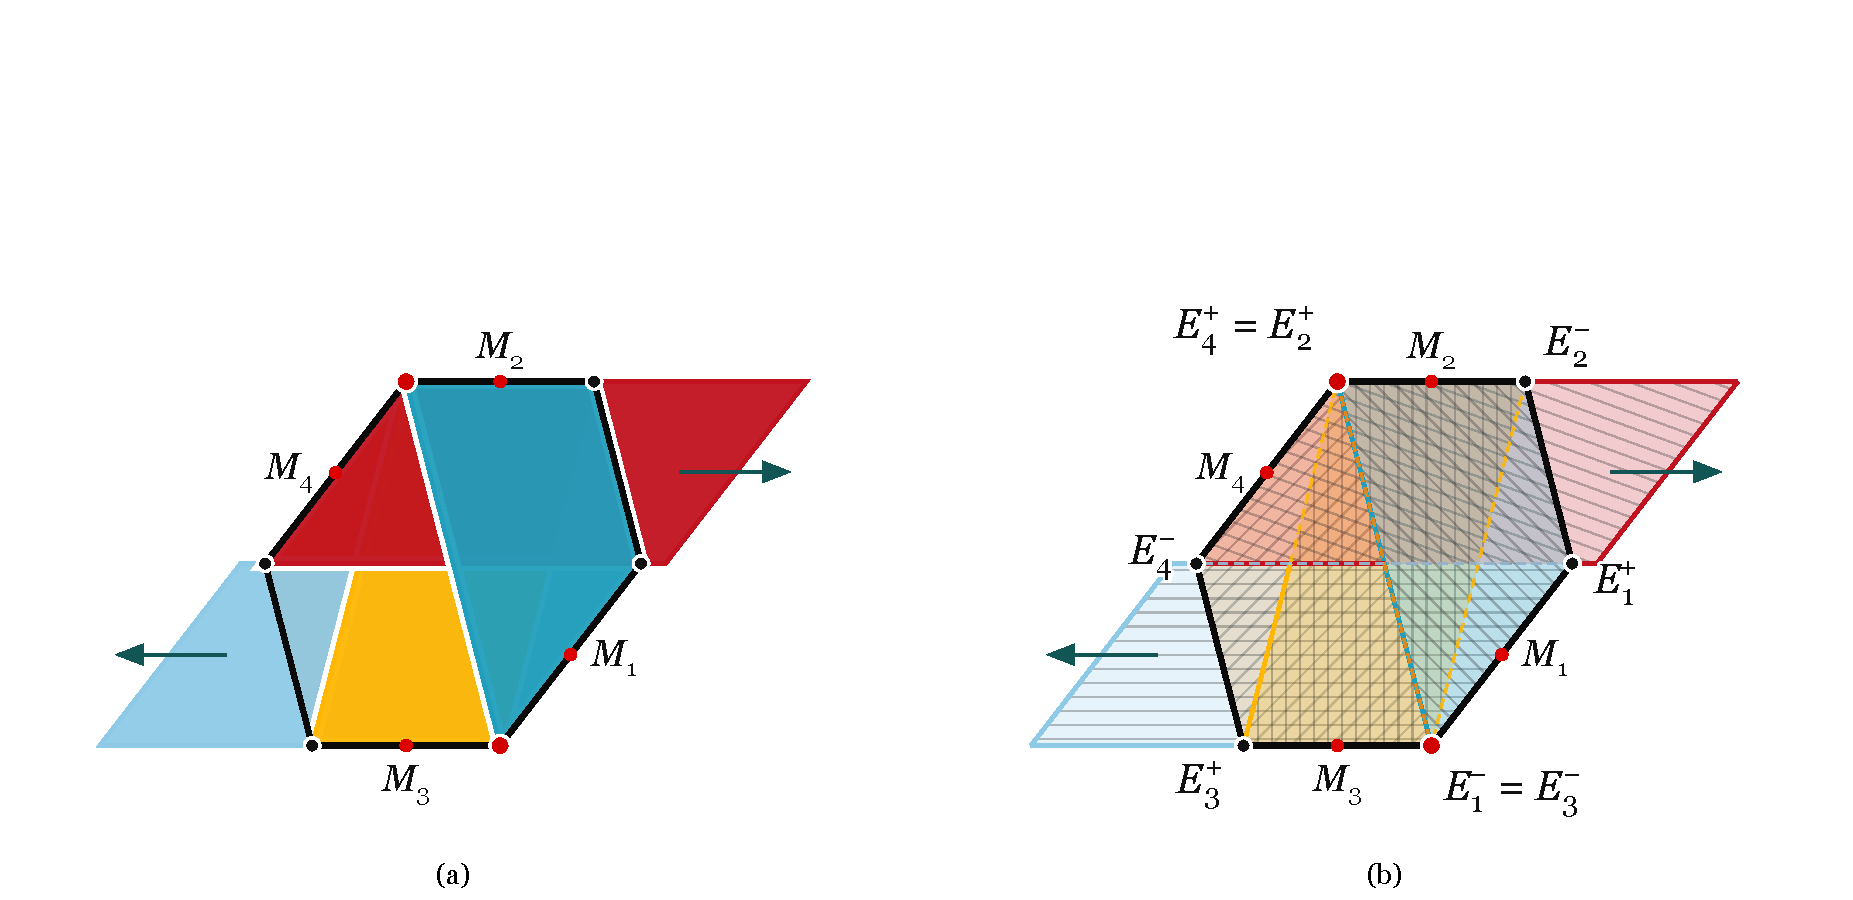
\includegraphics[width=0.85\linewidth]{figs/fig41-tight.pdf}
\caption{The exact figure-eight contact-chamber minimizer $\theta^*_{4_1}$. The core outline (heavy) is the centrally symmetric hexagon of Theorem~\ref{mainthm:hex}; its six sides are the four crease chords together with two band-edge segments, and the two red vertices are the double points $E_2^+=E_4^+$ and $E_1^-=E_3^-$ at which the crease chords close into a chain. The tails (arrows) leave in opposite directions, flush along the shared edge $y=\tfrac12$. All vertex coordinates lie in $\Q(\sqrt{15})$.}
\label{fig:f8tight}
\end{figure}

The shape describes the certified figure-eight contact-chamber minimizer (Figure~\ref{fig:f8tight}). The core outline is the hexagon with vertices
\begin{gather*}
\big({-}\tfrac{13\sqrt{15}}{30},\tfrac12\big),\qquad
\big({-}\tfrac{7\sqrt{15}}{30},\tfrac32\big),\qquad
\big(\tfrac{\sqrt{15}}{30},\tfrac32\big),\\
\big(\tfrac{\sqrt{15}}{10},\tfrac12\big),\qquad
\big({-}\tfrac{\sqrt{15}}{10},-\tfrac12\big),\qquad
\big({-}\tfrac{11\sqrt{15}}{30},-\tfrac12\big),
\end{gather*}
sides in the repeating pattern $\tfrac{2\sqrt{10}}5,\ \tfrac4{\sqrt{15}},\ \tfrac4{\sqrt{15}}$, twice around, interior angles $\arccos(-\tfrac14)\approx104.48^\circ$ at the two free crease endpoints and $\pi-\tfrac12\arccos(-\tfrac14)\approx127.76^\circ$ at the other four, perimeter $\tfrac{4\sqrt{10}}5+\tfrac{16}{\sqrt{15}}$, and area $\tfrac{4\sqrt{15}}5=\tfrac35\core(\theta^*_{4_1})$. It is not the regular hexagon. Its six sides are the four crease chords together with two band-edge segments, the exact four-crease analogue of the pentagon's three creases plus two edges; and the three core passes \emph{cover} it exactly, with overlap. After rescaling the $x$-coordinate by $2\sqrt{15}$, the $y$-coordinates being already rational, every vertex is rational, each panel is a convex quadrilateral whose vertices are vertices of the hexagon, so the union lies inside the hexagon. Exact inclusion--exclusion of rational areas, $12+16+12-8-8-0+0=24$, then shows the union exhausts it: no notch, by exact arithmetic, with mean overlap $\tfrac{40}{24}=\tfrac53$. The truncation length is also exact, under the same calibrated convention as for the trefoil---stubs measured to the point where each tail exits the core outline, the rule that reproduces \eqref{eq:kauffman-ratio}: each stub equals $L_1=\tfrac{2\sqrt{15}}5$ exactly, one more expression of the symmetry, giving
\[
\trunc(\theta^*_{4_1})=\tfrac{4\sqrt{15}}5+\tfrac{4\sqrt{15}}3=\tfrac{32\sqrt{15}}{15}=8.2623\ldots,
\qquad \frac{\trunc(\theta^*_{4_1})}{\core(\theta^*_{4_1})}=\frac85 .
\]
The outermost centreline crossing and the point at which a tail exits the outline give different stub lengths even for the trefoil. Cutting at the outline recovers \eqref{eq:kauffman-ratio}. For the figure-eight state the same convention gives $\tfrac{32\sqrt{15}}{15}=32/\sqrt{15}$, the value conjectured by Kauffman \cite{kauffman2004}. Theorem~\ref{mainthm:hex} establishes attainment, reachability from open valid states and strict local minimality of \emph{core length} on the stated contact chamber. For closed folded-ribbon conventions see \cite{denne2020,chen2025,yoo2026} and the crossing-number and four-page-index bounds \cite{kimnoyoo2026,yoo2026b}.

\begin{table}[tbp]
\centering\small
\renewcommand{\arraystretch}{1.15}
\begin{tabular}{p{0.58\linewidth}p{0.29\linewidth}}
\hline
\raggedright Figure-eight claim & \raggedright Verification grade\tabularnewline
\hline
\raggedright Actual-panel validity of $\theta^*_{4_1}$; hexagonal outline; core and truncation lengths & \raggedright exact\tabularnewline
\raggedright Valid opening path for $0<s\le10^{-3}$ & \raggedright exact inequalities on a continuous interval\tabularnewline
\raggedright Strict local minimum on the stated contact chamber $\mathcal C$ & \raggedright exact rank and positive KKT multipliers\tabularnewline
\raggedright Existence and uniqueness of the symmetric contact root in its specified box & \raggedright interval (Krawczyk)\tabularnewline
\raggedright Sampled cells, boundary inventory, descent endpoints and multistart KKT harvest & \raggedright numerical; finite search only\tabularnewline
\raggedright Necessity of the eight inequalities for every nearby valid state; exhaustive cell and root coverage & \raggedright not established\tabularnewline
\hline
\end{tabular}
\caption{Verification grades for the figure-eight results. The exact and interval certificates do not depend on the numerical search counts. The contact chamber $\mathcal C$ is defined by its eight explicit inequalities; the last row records the stronger statements that would extend the result beyond that chamber.}
\label{tab:figure8-grades}
\end{table}

\subsection{What the second instance teaches}
Three contrasts with the trefoil are worth stating plainly. First, the algebra collapsed: one more crossing, and the certified contact-chamber minimizer has quadratic coordinates, whereas the trefoil state has degree twelve with an associated sextic splitting group $S_6$. The trefoil's algebraic complexity occurs together with its notch---the record of a corner contact prised open along the second family---while at the figure-eight the central symmetry closes the crease chain exactly and no notch forms. These two examples suggest that the contact pattern, as well as the crossing number, matters to the algebraic complexity; they do not establish a general classification. Second, the phenomenology of the tails inverts: the tight trefoil sends its tails out at $69.5^\circ$---the $P_0P_3$ crossing angle of Remark~\ref{rem:gpaudit}---, the hexagonal figure-eight state sends them out antiparallel and flush, offset by exactly one strip width---consistent with the figure-eight's everyday use as a stopper knot that is loaded straight through. For a strip of width $w$ the prediction reads: hexagonal core with long sides $\approx1.265\,w$ and short sides $\approx1.033\,w$, consumed core material $\approx5.164\,w$, tails leaving antiparallel with zero gap. Third, both instances use the same verification grades and identify-then-verify procedure. Their geometric predicates still require separate checks: the four-crease computations use the actual oblique crease caps and unbounded tails, and their numerical searches are distinguished from the exact state and local-optimality certificates in Table~\ref{tab:figure8-grades}.

The numerical census has been rerun with the corrected actual-panel oracle. Of $4000$ boundary-probe attempts with seed $11$, $3995$ reach a boundary and all are assigned to the same eight endpoint-side contact labels; five attempts are rejected because the proposed starting state fails the current validity test. Both the boundary test and the event classification use oblique crease caps. This is a sampled inventory of the contacts active at $\theta^*_{4_1}$, not a proof that no other faces occur. Targeted minimization of $15$ crossing and length margins, from four revalidated starting states each, gives an overall observed minimum $0.5252598788\ldots$ in $56\,270$ trials. That observed value is not a global lower bound and does not exclude code walls from the valid closure.

The KKT rerun covers all $254$ nonempty subsets of at most seven of these eight contact functions, using seven initial values per subset: $1778$ Newton attempts. It returns $56$ convergence records, including repeated occurrences of the same root across seeds and subsets. Of these, $42$ have a negative multiplier and $14$ pass the nonnegative-multiplier filter; all $14$ lie within $3\times10^{-10}$ of $\theta^*_{4_1}$ in the seven chart coordinates. The residual stopping tolerance is $5\times10^{-8}$, the numerical approximate-closure distance tolerance is $10^{-6}$, and the multiplier tolerance is $10^{-8}$. Every root is checked against the actual panel oracle, independently of the sampled wall inventory. The exact candidate is validated separately below; neither convergence counts nor these numerical filters certify additional roots. Targeted searches of the other eight abstract cells, with $60$ restarts per cell and at most $4000$ steps per restart, find shadow realizations in four cells but no valid figure-eight state in any of the eight. These finite searches provide no emptiness proof. All original data, the unfiltered KKT records, final-predicate outcomes and source snapshots are retained in the ancillary repository; \texttt{scripts/reproduce-n4-search.sh} reproduces the full-size protocol.

Under the tangent half-angle substitution $u_i=\tan(\tau_i/2)$ the chart becomes rational, all eight walls become integer polynomials (degrees $7$ to $15$), the tight state keeps quadratic coordinates $u^*=(\sqrt{15}/3,\,\sqrt{15},\,-\sqrt{15},\,-\sqrt{15}/3)$ at which all eight polynomials vanish exactly, and a Krawczyk certificate on a box of radius $10^{-25}$ encloses $\theta^*_{4_1}$ with existence and uniqueness in its stratum. At the point itself validity is exact: \texttt{n4\_exact\_valid} builds all five actual panels from their side and crease half-planes, checks all six forbidden crease/pass pairs by clipping the full relative-open chord, and checks all nonadjacent centreline pairs. It uses no floating-point predicate to decide which constraints to include. Exact opening and Krawczyk certificates supplement this pointwise check; neither establishes global root coverage or all local contact branches.

The rerun leaves the proof obligations unchanged. Lemma~\ref{lem:wallcat} gives a finite \emph{candidate} catalogue of endpoint events and crease-pair contacts, but determining which occur as faces still requires per-event analysis, as performed for the trefoil in Corollary~\ref{cor:wallcomplete}. The Newton harvest does not establish per-stratum root completeness, and the sampled cells do not exhaust the geometric branch. Reachability, in contrast, is certified by Lemma~\ref{lem:slackstart41}. Extending contact-chamber optimality to the entire geometric cell requires a local tangent-cone argument at the simultaneous endpoint/cap contacts.

\section{Open problems}\label{sec:open}

\begin{enumerate}
\item\label{op:uniqueness}\emph{Proving global uniqueness.} After Theorem~\ref{thm:census} the principal numerical component is the per-stratum completeness of the harvest. The polynomialized wall system makes the exact route concrete: for $|S|=5$ the wall equations alone form a square polynomial system; for $|S|=4$ one adjoins the $\lambda$-eliminated determinant $\det[\nabla W_S\,|\,2D_p^2\nabla\ell]=0$; and for $|S|\le3$ the corresponding minor conditions. Each is a zero-dimensional system amenable to resultants, and the low-degree strata are the natural starting point. The obstruction is the trio of degree-$16$ walls $w_4,w_6,w_8$, which do however factor on partial loci, as the $N_5$ reduction already showed. A related missing ingredient is \emph{properness} of $\core$, that is, boundedness of its sublevel sets in the closure of $\M$; properness is what would turn ``a maximal pulling path converges to a tight state'' from a sketch into a theorem.

\item\label{op:lifting}\emph{Path-lifting.} Theorem~\ref{mainthm:realization} lifts individual states into slabs. Is there a theorem lifting an entire tightening path $p:[0,1]\to\M$ to a continuous family of realizations in a slab of \emph{fixed} height $\varepsilon>0$? On a compact subinterval inside an open stratum the budget $\varepsilon_0$ is continuous and positive, so one may take $\varepsilon<\min_t\varepsilon_0(p(t))$, and the ramp construction is itself a continuous function of the state; the open-interval case should reduce to a continuity statement about the existing construction, in the spirit of the monotone-path formalizations of \cite{cdr2003}. The hard end is $t\to1$: as the clearances are exhausted, the sufficient bound for this constant-height construction tends to zero. This does not rule out other realizations at the endpoint in a slab of fixed height; such an exclusion would require a separate lower-bound argument.

\item\label{op:thickness}\emph{Finite thickness.} Our realizations are $\varepsilon$-slab embeddings of a zero-thickness surface. A genuinely thick model---positive reach, a tubular neighbourhood of the sheet, contact forces in the sense of \cite{svdm2004,cks2002}---is a different and harder object. The relation between the two, and the correct notion of tightness for the thick model, is open.

\item\label{op:generaln}\emph{General $n$.} Which other four-crease cells contain tight states? The rational half-angle chart gives polynomial contact equations for comparing them with the certified hexagon. For $n\ge5$ the questions include the dimension, the wall catalogue, and whether truncation and core length select different states. Comparisons with closed ribbons \cite{denne2020,chen2025} require matching the length and closure conventions.

\item\label{op:creases}\emph{The complete-crease assumption.} We assume throughout that every crease is a chord joining the two long edges. Partial creases---corner folds---are excluded by a modelling decision, in line with the standard layer formalisms \cite{justin1997,hull2002,demaine2007}; whether they can matter for tying or for tightening is open.

\item\label{op:order}\emph{Sheet versus pointwise induced order.} Our definition of realization uses sheet separation. The pointwise form, comparing the heights of overlapping material points, is not known to be equivalent, and the pathology to exclude is a realization that pleats vertically inside the slab, through which the mod-$2$ argument behind the converse could leak. Two related gaps: strong $\varepsilon$-realization at a \emph{fixed} small $\varepsilon$ for a zero-clearance state, where the constant-height construction fails and a wedge-shaped height assignment is the natural candidate; and the formalization of the mod-$2$ crossing-parity lemma, whose proof uses standard mod-$2$ intersection theory \cite{gp1974} and which is the main target in formalizing the realization theory.

\item\label{op:kauffman}\emph{Kauffman's global conjecture.} Theorem~\ref{mainthm:kauffman} is local and confined to the three-crease branch. The global statement---that $4/\sqrt{5-2\sqrt5}$ is the minimum of $L/W$ over all flattened truncated trefoil ribbons \cite{kauffman2004}---is untouched. A natural intermediate step is to compare against branches with more creases, where the closed-ribbon results suggest that extra folds help for the closed functional; the immersed analogues \cite{immersed2020,ayala2025}, in which vertex tension balance plays the role of our wall-KKT balance, are the other obvious source of technique.

\item\label{op:formal}\emph{Formalization.} Sixteen algebraic core statements are machine-checked (Appendix~\ref{app:lean}). The bridge from that algebra to the geometry---coordinates, material topology, layer order, wall definitions---is not formalized, and the mod-$2$ crossing-parity lemma, standard in content \cite{gp1974}, is the identified hard case for formalization.
\end{enumerate}

\appendix

\section{The verification suite}\label{app:suite}

Structural claims were first explored numerically in double precision and then promoted through higher-precision evaluation ($40$--$80$ digits), algebraic identification, exact quotient-field verification, interval arithmetic for existence and signs, and Lean~4 proofs for the supporting algebraic core. Integer-relation detection \cite{fba1999} served only as a search heuristic; every candidate expression it proposed was either verified as an exact identity or discarded.

Exact verification is carried out in the quotient field $\Q[x]/(p_x)$, and in $\Q(x_0)$ or $\Q(x)$ where the pentagon or a general state is concerned, without heuristic numerical simplification (\texttt{nsimplify}) or floating-point sign calibration. A recursive evaluator reduces rational expressions to canonical representatives modulo the minimal polynomial, so claimed identities are decided by exact reduction to $0$ rather than tolerance checks. For inequalities and existence assertions we use outward-rounded interval arithmetic \cite{neumaier1990}: Krawczyk and interval-Newton enclosures on boxes of radius $10^{-20}$ to $10^{-50}$ at $40$- to $80$-digit precision, together with interval evaluation for positivity of multipliers, the reduced Hessian, and census wall margins. The mutation suite (\texttt{test\_guards}) runs ten original certificates and their altered copies in default and optimized Python. Each altered copy must exit with its expected mathematical diagnostic. Structurally important computations are cross-checked by independent routes---rational expression trees versus polynomialized walls, symbolic differentiation versus an $80$-digit second difference (agreeing to $4.7\times10^{-34}$), and \texttt{mpmath} versus \textsc{Arb} ball arithmetic (\texttt{arb\_recheck}).

Table~\ref{tab:suite} lists the principal certificate for each result. The historical probes in the reproducibility guide include the endpoint-sampling counterexample of Remark~\ref{rem:methods}.

The companion distribution \cite{anc} contains the source files and dependency locks, the recorded numerical checkpoints, and SHA-256 manifests for the calculations, logs and artifacts.

\begin{table}[tbp]
\centering\small
\renewcommand{\arraystretch}{1.15}
\begin{tabular}{@{}>{\raggedright\arraybackslash}p{0.445\linewidth}@{\hspace{0.035\linewidth}}>{\raggedright\arraybackslash}p{0.52\linewidth}@{}}
\hline
Result and scope & Principal verification scripts\\
\hline
A. Alternating trefoil word, slope signs and local/global layer order &
\texttt{check\_gauss}, \texttt{check\_gp}, \texttt{exact\_common\_overlap}\\
B. Slice identities, chart and contact walls &
\texttt{exact\_slice}, \texttt{exact\_taco}, \texttt{exact\_common\_overlap}\\
C. Inward slope $-1/20$, monotone descent and crossing preservation &
\texttt{exact\_core\_descent}, \texttt{exact\_reach}, \texttt{exact\_branch}\\
D. Degree twelve, stationarity and positive reduced curvature at $\td$ &
\texttt{exact\_field}, \texttt{exact\_unique\_h}, \texttt{exact\_kkt\_dagger}, \texttt{exact\_second}\\
D and Section~\ref{sec:shape}. Seven-sided outline and notch &
\texttt{exact\_outline}, \texttt{exact\_notch}\\
E. Truncation minimum and flush-cut edges at $P^*$ &
\texttt{exact\_kauffman2}, \texttt{exact\_trunc\_nbhd}\\
F. Opening at both distinguished states and the cyclic local-order example &
\texttt{exact\_opening}, \texttt{exact\_common\_overlap}\\
G. Wall exclusion on $72$ isolated root boxes and classification of $32$ inconclusive centres &
\texttt{exact\_census\_roots} (Arb), using the saved harvest from \texttt{uniq\_census}\\
H. Figure-eight validity, opening, stationarity, chamber minimum and hexagon &
\texttt{n4\_exact\_valid}, \texttt{n4\_exact\_opening}, \texttt{n4\_exact\_kkt}, \texttt{n4\_exact\_local}, \texttt{n4\_krawczyk}, \texttt{n4\_certify}\\
H. Combinatorial enumeration and recorded numerical search &
\texttt{n4\_cells3}, \texttt{check\_n4\_geometry}, \texttt{check\_n4\_rerun}\\
\hline
\end{tabular}
\smallskip\caption{Computational evidence for Theorems A--H. The reproducibility guide gives the commands, inputs and expected results. The last row includes a finite numerical search.}
\label{tab:suite}
\end{table}

\FloatBarrier
\section{Lean formalization}\label{app:lean}

Sixteen statements forming the algebraic core of the paper are machine-checked in Lean~4 against Mathlib \cite{mathlib2020}, in two files. The nine theorems of \texttt{Pentagon.lean} formalize the slice: the closed form of the gap $\Delta$, the sum-of-squares identity behind the positivity of the numerator of $\Delta'$, the strict positivity of the slice polynomial $p$ on $y>0$, the characterization and the uniqueness of the contact root in the relevant range, the implication from that root to $|EH|^2=|EF|^2$, a root-of-unity closure lemma, and the closed form and strict monotonicity of $\core$ along the slice---together, supporting algebra for the folklore half of Theorem~\ref{mainthm:pass}, without a formal polygon or angle model. The seven theorems of \texttt{ThetaDagger.lean} formalize the second family: the field identity $\ell=h+b$ as an exact equality of polynomials, the monotonicity package for the defining polynomial, existence of its root in $(0.32,0.33)$ by the intermediate value theorem together with uniqueness in $(0,1)$, and the certificate separating the pentagon from $\td$, discharged by \texttt{linear\_combination} on explicit certificate polynomials. Table~\ref{tab:lean} lists them; there, $P(x)=5x^4-10x^2+1$ is the pentagon contact polynomial, $p$ denotes the slice polynomial in $y=x^2$ in the \texttt{Pentagon} rows and the defining polynomial of the second family in the \texttt{ThetaDagger} rows, and equal statement names in the two files are distinct namespaced theorems.

\begin{table}[t]
\centering\small
\begin{tabular}{@{}ll@{}}
\hline
Theorem & Content\\
\hline
\multicolumn{2}{@{}l}{\emph{\texttt{Pentagon.lean}}, nine theorems}\\
\texttt{delta\_formula} & closed form of the gap $\Delta$\\
\texttt{deriv\_numerator\_pos} & positivity of the numerator of $\Delta'$ (SOS identity)\\
\texttt{p\_pos} & $p(y)>0$ for $y>0$\\
\texttt{x0\_root} & $s^2=5$ and $sx^2=s-2$ imply $P(x)=0$\\
\texttt{root\_unique} & uniqueness of the root in the range $y<\frac13$\\
\texttt{side\_eq\_of\_contact} & $P(x)=0$ implies $((1-3x^2)/(2x))^2=1+x^2$\\
\texttt{closure\_root\_of\_unity} & $1+z+\dots+z^4=0$ implies $z^5=1$\\
\texttt{ell\_core\_closed\_form} & $\core=\frac1x-x$ on the slice\\
\texttt{ell\_core\_strict\_anti} & strict decrease of $\core$ along the slice\\
\hline
\multicolumn{2}{@{}l}{\emph{\texttt{ThetaDagger.lean}}, seven theorems}\\
\texttt{ell\_eq\_h\_add\_b} & the identity $\ell=h+b$ as an equality in $\Q[x]$\\
\texttt{deriv\_pos} & $p'>0$ on $(0,1]$\\
\texttt{p\_hasDerivAt} & the derivative formula for $p$\\
\texttt{p\_strictMonoOn} & $p$ strictly increasing on $[0,1]$\\
\texttt{root\_exists} & existence of a root in $(0.32,0.33)$\\
\texttt{root\_unique} & uniqueness of that root in $(0,1)$\\
\texttt{pentagon\_not\_thetaDagger} & the saddle--well separation certificate\\
\hline
\end{tabular}
\caption{The sixteen machine-checked statements, grouped by file.}
\label{tab:lean}
\end{table}

What is machine-checked is the \emph{algebraic} content of these statements. The bridge from that algebra to the geometry of a folded strip---the coordinate setup, the material topology, the layer order, the wall definitions---remains human proof supported by exact symbolic derivation. Formalizing that bridge is a large project; it is not claimed here, and its identified hard case is recorded as open problem~\ref{op:formal}.


\section*{Data and code availability}
All symbolic derivations, interval certificates, verification logs, and Lean sources used in this paper are collected in the ancillary repository \cite{anc}, publicly available at \url{https://github.com/yongsk0066/flat-overhand-knot}, together with pinned interpreter and library versions, SHA-256 manifests for every certificate input and log, a theorem-to-script correspondence (Table~\ref{tab:suite}), and step-by-step reproduction instructions. A Zenodo DOI at a fixed Git commit will be minted at submission, and the entry \cite{anc} updated to the archived version.

\section*{Use of generative AI}
Generative AI tools were used during exploratory investigation, manuscript drafting and editing, internal adversarial review, and candidate-reference search. All definitions, computations, proofs, certificates, software outputs, citations, and final claims were independently verified and remain the sole responsibility of the author.

\bibliographystyle{amsalpha}
\bibliography{references}

\end{document}
